% !Mode:: "TeX:UTF-8"
%# -*- coding:utf-8 -*-

%% 南京大学学位论文的示例文档
%% 作者:njuhan: https://github.com/njuHan
%% 源模版repo: https://github.com/njuHan/njuthesis-nju-thesis-template

\documentclass[winfonts,master,oneside]{njuthesis}
%% 审阅模式很重要,命令是下方使用的/blind
%% njuthesis 文档类的可选参数有:
%%   winfonts, linuxfonts, macfonts, adobefonts winfonts 选项使得文档使用Windows 系统提供的字体;linuxfonts 选项使得文档使用Linux 系统提供的字体;macfonts 选项使得文档使用Mac 系统提供的字体;adobefonts 选项使得文档使用Adobe提供的OTF中文字体(需自行下载安转)
%%   phd/master/bachelor 选择博士/硕士/学士论文
%%   twoside 或 oneside 指定排版的文档为双面打印或单面打印格式(twoside会使得chapter 章节从奇数页开始,即纸张的正面开始,因此会出现一些空白的页面)
%%   nobackinfo 取消封二页导师签名信息。注意,按照南大的规定,是需要签名页的。

\usepackage{pdfpages}
\usepackage{listings}
% \usepackage{ctex}
\usepackage{tabularx}
\usepackage{float}
% \usepackage{subfigure}
\lstset{
    basicstyle          =   \ttfamily,          % 基本代码风格
    keywordstyle        =   \bfseries,          % 关键字风格
    commentstyle        =   \rmfamily\itshape,  % 注释的风格,斜体
    stringstyle         =   \ttfamily,  % 字符串风格
    flexiblecolumns,                % 别问为什么,加上这个
    %numbers             =   left,   % 行号的位置在左边
    showspaces          =   false,  % 是否显示空格,显示了有点乱,所以不现实了
    numberstyle         =   \zihao{-5}\ttfamily,    % 行号的样式,小五号,tt等宽字体
    showstringspaces    =   false,
    captionpos          =   t,      % 这段代码的名字所呈现的位置,t指的是top上面
    frame               =   lrtb,   % 显示边框
}
%%%%%%%%%%%%%%%%%%%%%%%%%%%%%%%%%%%%%%%%%%%%%%%%%%%%%%%%%%%%%%%%%%%%%%%%%%%%%%%
% set up labelformat and labelsep for subfigure 详见: http://www.latexstudio.net/archives/8652.html
\captionsetup[subfigure]{labelformat=simple, labelsep=space}

%%%%%%%%%%%%%%%%%%%%%%%%%%%%%%%%%%%%%%%%%%%%%%%%%%%%%%%%%%%%%%%%%%%%%%%%%%%%%%%
% 设置《国家图书馆封面》的内容,仅博士论文才需要填写

% 设置论文按照《中国图书资料分类法》的分类编号
%\classification{0175.2}
% 设置论文按照《国际十进分类法UDC》的分类编号
% 该编号可在下述网址查询:http://www.udcc.org/udcsummary/php/index.php?lang=chi
%\udc{004.72}
% 国家图书馆封面上的论文标题第一行,不可换行。此属性可选,默认值为通过\title设置的标题。
%\nlctitlea{论文标题第一行}
% 国家图书馆封面上的论文标题第二行,不可换行。此属性可选,默认值为空白。
%\nlctitleb{论文标题第二行}
% 国家图书馆封面上的论文标题第三行,不可换行。此属性可选,默认值为空白。
%\nlctitlec{}
% 导师的单位名称及地址
%\supervisorinfo{南京大学计算机科学与技术系~~南京市汉口路22号~~210093}
% 答辩委员会主席
%\chairman{张三丰~~教授}
% 第一位评阅人
%\reviewera{阳顶天~~教授}
% 第二位评阅人
%\reviewerb{张无忌~~副教授}
% 第三位评阅人
%\reviewerc{黄裳~~教授}
% 第四位评阅人
%\reviewerd{郭靖~~研究员}


%%%%%%%%%%%%%%%%%%%%%%%%%%%%%%%%%%%%%%%%%%%%%%%%%%%%%%%%%%%%%%%%%%%%%%%%%%%%%%%
% 设置论文的中文封面

% 单行论文标题,不可换行
\title{}
\titlea{全动飞行模拟视景系统中}
\titleb{数据交换子系统的设计与实现}
% 如果论文标题过长,可以分两行,第一行用\titlea{}定义,第二行用\titleb{}定义,
% 使用以下3行:
%\title{} %用于覆盖单行标题内容为空
%\titlea{长标题第一行}  %第一行标题写这里
%\titleb{长标题第二行用于长标题换行} %第二行标题写这里
% 注意: \title 不能都注释,它用于控制标题选择双行还是单行。\title{}如果内容为空,则编译\titlea{},titleb{}双行标题,否则编译单行标题


% 论文作者姓名
\author{陈氢}
% 论文作者联系电话
\telphone{19821233104}
% 论文作者电子邮件地址
\email{mf21320019@smail.nju.edu.cn}
% 论文作者学生证号
\studentnum{MF21320019}
% 论文作者入学年份(年级)
\grade{2021}
% 论文作者毕业年份(届), 出版授权书的学位年度
\graduateyear{2023}
% 导师姓名职称
\supervisor{冯桂焕副教授}
% 导师的联系电话
\supervisortelphone{}
% 论文作者的学科与专业方向
\major{工程硕士(软件工程领域)}
% 论文作者的研究方向
\researchfield{软件工程}
% 论文作者所在院系的中文名称
\department{软件学院}
% 论文作者所在学校或机构的名称。此属性可选,默认值为``南京大学''。
\institute{南京大学}
% 论文的提交日期,需设置年、月、日。
\submitdate{xxxx年 xx 月 xx 日}
% 论文的答辩日期,需设置年、月、日。
\defenddate{xxxx年 xx 月 xx 日}
% 论文的定稿日期,需设置年、月、日。
% 此属性可选,若注释\date{},则默认值为最后一次编译时的日期,精确到日。
% \date{2019年5月20日}

%%%%%%%%%%%%%%%%%%%%%%%%%%%%%%%%%%%%%%%%%%%%%%%%%%%%%%%%%%%%%%%%%%%%%%%%%%%%%%%
% 设置论文的英文封面

% 论文的英文标题,不可换行
\englishtitle{Design and Implementation of Data Exchange Subsystem in Full Flight Simulator Visual System }
% 论文作者姓名的拼音
\englishauthor{Chen Qing}
% 导师姓名职称的英文
\englishsupervisor{Professor Feng Guihuan}
% 论文作者学科与专业的英文名
\englishmajor{Software Engineering}
% 论文作者所在院系的英文名称
\englishdepartment{Software Institute}
% 论文作者所在学校或机构的英文名称。此属性可选,默认值为``Nanjing University''。
\englishinstitute{Nanjing University}
% 论文完成日期的英文形式,它将出现在英文封面下方。需设置年、月、日。日期格式使用美国的日期
% 格式,即``Month day, year'',其中``Month''为月份的英文名全称,首字母大写;``day''为
% 该月中日期的阿拉伯数字表示;``year''为年份的四位阿拉伯数字表示。
% 此属性可选,若注释掉\englishdate{},则默认值为最后一次编译时的日期。
% \englishdate{May 20, 2019}

%%%%%%%%%%%%%%%%%%%%%%%%%%%%%%%%%%%%%%%%%%%%%%%%%%%%%%%%%%%%%%%%%%%%%%%%%%%%%%%
% 设置论文的中文摘要

% 设置中文摘要页面的论文标题及副标题的第一行。
% 此属性可选,其默认值为使用|\title|命令所设置的论文标题
\abstracttitlea{全动飞行模拟视景系统中数据交换子系统}
% 设置中文摘要页面的论文标题及副标题的第二行。
% 此属性可选,其默认值为空白
\abstracttitleb{的设计与实现}

%%%%%%%%%%%%%%%%%%%%%%%%%%%%%%%%%%%%%%%%%%%%%%%%%%%%%%%%%%%%%%%%%%%%%%%%%%%%%%%
% 设置论文的英文摘要

% 设置英文摘要页面的论文标题及副标题的第一行。
% 此属性可选,其默认值为使用|\englishtitle|命令所设置的论文标题
\englishabstracttitlea{Design and Implementation of Data Exchange Subsystem}
% 设置英文摘要页面的论文标题及副标题的第二行。
% 此属性可选,其默认值为空白
\englishabstracttitleb{in Full Flight Simulator Visual System}

%%%%%%%%%%%%%%%%%%%%%%%%%%%%%%%%%%%%%%%%%%%%%%%%%%%%%%%%%%%%%%%%%%%%%%%%%%%%%%
%% 盲审命令,空白字段设置请看 .cls文件 \newcommand*{\blind}
%% 此外,请按照盲审要求自行去掉个人简历、致谢等页面中的个人信息
%%**********************!!!非常重要的盲审命令,送审前必选!!!****************
%\blind
%%**********************!!!非常重要的盲审命令,送审前必选!!!****************

%%%%%%%%%%%%%%%%%%%%%%%%%%%%%%%%%%%%%%%%%%%%%%%%%%%%%%%%%%%%%%%%%%%%%%%%%%%%%%%
\begin{document}

%%%%%%%%%%%%%%%%%%%%%%%%%%%%%%%%%%%%%%%%%%%%%%%%%%%%%%%%%%%%%%%%%%%%%%%%%%%%%%%

% 制作国家图书馆封面(博士学位论文才需要)
%\makenlctitle
% 制作中文封面
\maketitle
% 制作英文封面
\makeenglishtitle


\includepdf{chapter/statement.pdf}
%%%%%%%%%%%%%%%%%%%%%%%%%%%%%%%%%%%%%%%%%%%%%%%%%%%%%%%%%%%%%%%%%%%%%%%%%%%%%%%
% 开始前言部分
\frontmatter
\begin{abstract}
    {飞行模拟不只是普罗大众概念里一类体验飞行环游的游戏,
    其同时肩负着飞行训练这一更严肃使命。依托全动飞行模拟机进行日常训练是每一位飞行员的重要科目。
    达到飞行训练要求的模拟机称为全动飞行模拟机。
    目前我国的相关设备基本依赖进口,近年来国际局势剧烈变动,加之中国商飞C919客机取得中国民航局颁发的合格证,相应全动飞行模拟机的自主研发必须快马加鞭。
    \par
    本项目立足于自主研发的全动飞行模拟机中承担视觉效果的视景系统。
    仿真机是一台模拟机的核心,视景系统的运作需要仿真机的指令驱动。
    然而进口仿真机并不对外开放接口,为了基于其开发视景系统,本文首先通过网络流量分析的方法结合文档发现仿真机网络最高层为数据链路层,
    并解读了仿真机与视景系统沟通的二十余种指令信息。
    为了将视景系统接入该仿真机,在数据交换子系统中设计并实现了充当仿真机网络协议栈、多种指令转化以及与视景系统的图像生成器沟通等功能。
    过程中使用到ProtoBuffer协议来提升交换效率,设计了自定义指令集屏蔽仿真机间的差异。
    \par
    在初步测试中,数据交换子系统可以正确处理并传递已解读的指令。然而也发现在需要连接多台图像生成器融合投影的情况下,图像的拼接部分有撕裂,抖动的现象。
    经过分析排查后,引入了网络帧缓存和插值机制,实现多图像生成器的数据同步与平滑,改善了投影效果。
    目前该视景系统可以在CAE仿真机操控下,以至少60帧率实现地景数据库中各机场附近环绕飞行,标志着迈出了动起来的坚实第一步。以此为根基,后续对天气、灯光、植被等多种系统进行研究与引入,尽早达成训练用模拟机的验收标准。
    }          
	\keywords{飞行模拟;视景系统;数据交换;数据同步}          
\end{abstract}


%%%%%%%%%%%%%%%%%%%%%%%%%%%%%%%%%%%%%%%%%%%%%%%%%%%%%%%%%%%%%%%%%%%%%%%%%%%%%%%
% 论文的英文摘要
\begin{englishabstract}
	{Flight simulation in most people's concept may be a kind of game to experience flight. 
    However, it's a more significant function for flight simulation to assist flight training. Daily training by professional simulator is an important subject for every pilot.
    The simulator that meets the requirements of flight training is called Full Flight Simulator(FFS).
    Currently, the FFS equipment of China depends on imports. FFS independent research and development must be accelerated because the international situation has changed dramatically and 
    the COMAC C919 has received a certificate from the Civil Aviation Administration of China.
    
    \par
    This project is based on the self-developed visual system who undertakes visual effects of FFS. 
    The visual system needs to be driven by the instructions of imitator, which is the core of a simulator.
    However, the imported imitators do not open the interface. In order to develop the visual system based on it, 
    through the method of network traffic analysis and documents in this paper, it is found that the top layer of the imitator network is the data link layer.
    At the same time, we verify more than 20 kinds of instruction that the imitator communicates with the visual system.
    In the data exchange subsystem, functions such as acting as the network protocol stack of the imitator, converting various instructions and communicating with the image generator of the visual system are designed and implemented, for the sake of connecting the visual system to the imitator.
    The ProtoBuffer protocol is used to improve the data exchange efficiency, and a user-defined instruction set is designed to shield the discrepancies between the imitators.
    \par
    In preliminary tests, the data exchange subsystem is able to correctly process and deliver the verified instructions.
    However, it is also found that the splicing part of the image has screen tearing and jitter when multiple image generators are connected.
    To improve projection effect, the network frame cache and interpolation mechanism are introduced to realize data synchronization and smoothing in multiple image generators.
    At present, under the control of CAE imitator, the system realizes the circling flight around airports in the landscape database at least 60 frame rate. The flying plane in the visual system marks a crucial first step.
    The next step is to study and introduce weather, lighting, vegetation and other systems, so as to up to standard of D-Level simulator as soon as possible.
    }
    % 英文关键词。关键词之间用英文半角逗号隔开,末尾无符号。
	\englishkeywords{Flight Simulation, Visual System, Data Exchange, Data Synchronism}
\end{englishabstract}

%%%%%%%%%%%%%%%%%%%%%%%%%%%%%%%%%%%%%%%%%%%%%%%%%%%%%%%%%%%%%%%%%%%%%%%%%%%%%%%
% 论文的前言,应放在目录之前,中英文摘要之后,一般不需要
%
%\begin{preface}
%
%在过去的40年中,手写中文文本领域识别(HCTR)取得了很大的进展[1,2]。
%
%\vspace{1cm}
%\begin{flushright}
%饶安逸\\
%2018年5月15日于南大仙林
%\end{flushright}
%
%\end{preface}

%%%%%%%%%%%%%%%%%%%%%%%%%%%%%%%%%%%%%%%%%%%%%%%%%%%%%%%%%%%%%%%%%%%%%%%%%%%%%%%
% 生成论文目录
\tableofcontents

%%%%%%%%%%%%%%%%%%%%%%%%%%%%%%%%%%%%%%%%%%%%%%%%%%%%%%%%%%%%%%%%%%%%%%%%%%%%%%%
% 生成插图清单。如无需插图清单则可注释掉下述语句。
\listoffigures

%%%%%%%%%%%%%%%%%%%%%%%%%%%%%%%%%%%%%%%%%%%%%%%%%%%%%%%%%%%%%%%%%%%%%%%%%%%%%%%
% 生成附表清单。如无需附表清单则可注释掉下述语句。
\listoftables

%%%%%%%%%%%%%%%%%%%%%%%%%%%%%%%%%%%%%%%%%%%%%%%%%%%%%%%%%%%%%%%%%%%%%%%%%%%%%%%
% 开始正文部分
\mainmatter

%%%%%%%%%%%%%%%%%%%%%%%%%%%%%%%%%%%%%%%%%%%%%%%%%%%%%%%%%%%%%%%%%%%%%%%%%%%%%%%
% 学位论文的正文应以《绪论》作为第一章,本模板是按照自身功能模块组织的,并非论文中的章节安排

\chapter{引言}
\section{项目背景}
1920年我国第一条民用航线开航,一百年后飞机早已是寻常百姓家的出行选择。《2021年全国民用运输机场生产统计公报》\cite{minhang}显示,2021年我国境内民用机场已达248个,在地域广袤的中西部,机场几乎是城市标配。
同时《2022年度全球民航航班运行报告》\cite{variflight}显示,新冠疫情背景下2022年度国内航线实际执行客运航班量仍达239万架次,且相比2019年疫情前刚恢复五成以上。航空较陆路有更复杂的安全因素,民用航班的普及离不开航空安全的精进。据《国际航协2021年全球航空运输安全报告》\cite{iata}统计,2021年客机所属涡轮螺旋桨飞机每百万次飞行发生1.77起损毁,5年内平均值
为1.22。这一方面得益于成熟的飞机制造,另一方面全动飞行模拟机(Full Flight Simulator 以下简称为 FFS)为飞行员提供身临其境的训练环境功不可没。
\par
FFS是由模拟座舱、视景系统、声音系统、运动系统、网络系统和仿真机构成的飞行训练工具\cite{simulator3}。汽车驾驶员可以驾驶符合驾照类别的任意汽车,而民航飞行员想获取某型号飞机的驾驶资格,必须在对应型号FFS上进行日常训练。因此新机型若想步入市场,配套FFS不可或缺。我国航空市场广阔,且国产大飞机C919已蓄势待发,FFS需求旺盛,但目前该领域仍主要依靠行业巨擘加拿大CAE公司。
进口产品购置成本高,二次开发困难,且可能面临技术封锁。为降低成本与风险,FFS的国产化迫在眉睫。
\par
本文中基于自研游戏引擎开发的视景系统是最终实现FFS国产化的重要组成部分。
一台FFS的核心是仿真机,它相当于整个FFS的后台,负责根据飞行员在模拟座舱中的输入操作计算生成各类指令。各个系统运作均由来自仿真机的指令控制。视景系统负责根据仿真机指令中的位置信息从地景数据库中加载周边地形地貌,并结合时间,天气等综合信息实时渲染座舱前方的仿真景象;飞行中产生的如碰撞等异常行为也由视景系统反馈给仿真机。
由此可见开发视景系统离不开仿真机的支持,本视景系统便是基于国内占有量最高的CAE仿真机开发。
\par
但作为拥有行业主导地位的进口设备,CAE仿真机本就不打算搭载除本公司以外的视景系统,它们之间通过怎样的接口通信毫无说明。为了将自研视景系统成功接入该仿真机,需要先理解仿真机的指令,再实现与方便视景系统使用的自定义指令间的转换方法,才能让双方成功交流,这便是数据交换子系统要承担的任务。
此外有了该子系统帮助翻译,一定程度上屏蔽了仿真机侧的差异,为视景系统的通用性留下余地。
% \par
% 经过对多种仿真机抓包分析后,发现问题在于仿真机是一个非常底层的设备,从网络模型角度看其最高层是数据链路层,指令数据用以太网协议封装后便进行发送,接收数据也只能仅被以太网协议封装过,否则无法正确解读。因此无法通过工作于传输层以上的传统socket连接模式与本视景系统中的图像生成器交流。
% 为了使位于不同网络体系结构层级的仿真机与图像生成器沟通,本文为视景系统设计了数据交换子系统。一方面连接仿真机,收发仅用以太网协议封装的数据帧,转换为自拟指令类型后,通过传统网络体系层层封装再与图像生成器交互。
% 这不仅解决了图像生成器与仿真机的交流问题,还屏蔽了不同厂商仿真机间数据组织结构的差异,保留了搭载于多种仿真机上的可能。
% \par
% 其次在真实训练环境下,模拟座舱前方是一个球幕,需要多个图像生成器同时工作进行融合投影才能产生良好的视觉效果。但出于网络波动和TCP仅支持单播的特点,数据到达各图像生成器的时间存在差异,导致最终的融合投影产生画面撕裂。
% 为解决该问题,在图像生成器侧设计了网络帧缓冲机制和多种插值方法,使得多台设备逻辑线程可以做到几乎同时使用相同的数据进行计算。
\par
目前本视景系统以适配国内仍大量服役的进口仿真机为短期目标,同时也为搭载于孕育中的国产仿真机做准备,期待国产FFS能够早日走进各大飞行训练基地。
\section{国内外相关技术的发展概况}
\subsection{飞行模拟机}
世界上第一架飞机于1903年由莱特兄弟试飞成功,最初的飞行模拟机则诞生于1910年,仅具备三个维度的手动旋转功能\cite{simhis1}。 1917年,法国的Lender和Heildelbergof发明了燃油驱动旋转的版本\cite{simhis2}。而现代飞行模拟机的雏形则是发明于1930纯电气驱动的Linker Trainer,它在1937年被美国航空公司引入。
之后在二战爆发和电子计算机兴起的刺激下,飞行模拟机逐渐发展出更复杂体系和更真实的感官效果\cite{simulator2}。最终发展为现在这种以飞行员在座舱中的操作为输入,仿真机根据输入计算各种状态,再以指令的形式驱动视景、声音、运动等系统工作的结构。
\par
现代飞行模拟机的种类很多,从大的方面来看,基本可以分为试验用飞行模拟机和训练用飞行模拟机两大类。
试验用飞行模拟机主要用于新型飞机研制或旧机型改进。
训练用飞行模拟机早已拥有完备的标准。国际民航组织ICAO于1995年发布《飞行模拟鉴定标准手册》并持续更新\cite{normalize2},所有现代商业飞行模拟机均需要按照标准设计,通过鉴定后才可以用于飞行员培训。我国于2005年由中国民用航空总局正式颁发的CCAR-60《飞行模拟设备的鉴定和使用规则》作为
国内航空公司飞行员模拟训练设备的鉴定标准,并于2019年重新修订\cite{normalize1}。《规则》中说明我国训练用飞行模拟机分为A、B、C、D四个等级,其中D级为最高标准,即要达成《规则》文件中的全部最高标准,
才可以作为全程飞行训练的模拟机。C、B、A三个等级则是在响应时间,功能完整性方面逐步放宽要求,可以用于一些专项训练。
表\ref{viscomp}提供了《规则》中视景系统部分标准的对比。图\ref{simout}与图\ref{siminn}提供了D级模拟机外部和内部样貌。
\begin{table}[h!]
    \begin{center}
        \caption{视景系统部分标准对比}
        \label{viscomp}
        \renewcommand\arraystretch{1.2}
        \begin{tabularx}{\textwidth}{ 
            | >{\centering\arraybackslash\hsize=0.5\hsize\linewidth=\hsize}X 
            | >{\centering\arraybackslash\hsize=0.125\hsize\linewidth=\hsize}X 
            | >{\centering\arraybackslash\hsize=0.125\hsize\linewidth=\hsize}X 
            | >{\centering\arraybackslash\hsize=0.125\hsize\linewidth=\hsize}X 
            | >{\centering\arraybackslash\hsize=0.125\hsize\linewidth=\hsize}X 
            | }
            \hline
            \textbf{视景系统要求} & \textbf{A} & \textbf{B} & \textbf{C} & \textbf{D}\\
            \hline
            视景系统不应具有导致不真实特性的光学不连续性和人工痕迹。 & √ & √ & √ & √\\
            \hline
            模拟机应当在每个驾驶员座位上提供连续最小水平90°、垂直40°的准直视场。 & & & √ & √\\
            \hline
            视景系统应当提供着陆期间判断下降率(深度感觉)所必须的目视提示。 & & √ & √ & √\\
            \hline
            提供黄昏和黎明视景,保证环境光强度减弱的色彩表征。 & & & √ & √\\
            \hline
            模拟机应当能在起飞、进近和着陆期间表现雷暴附近的轻度、中度和重度降水的特殊天气。 & & & & √\\
            \hline
            模拟机应当表现全部机场灯光的真实颜色和方向性。 & & & & √\\
            \hline
        \end{tabularx}
    \end{center}
\end{table}
\begin{figure}[h!]
    \begin{minipage}[t]{0.48\textwidth}
        \centering
        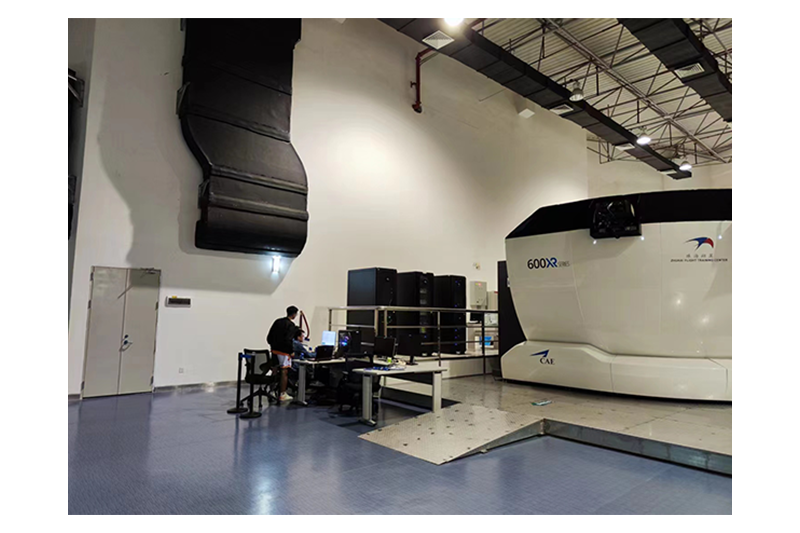
\includegraphics[width=6cm]{pictures/simulator.png}
        \caption{D级模拟机外部}
        \label{simout}
    \end{minipage}
    \begin{minipage}[t]{0.48\textwidth}
        \centering
        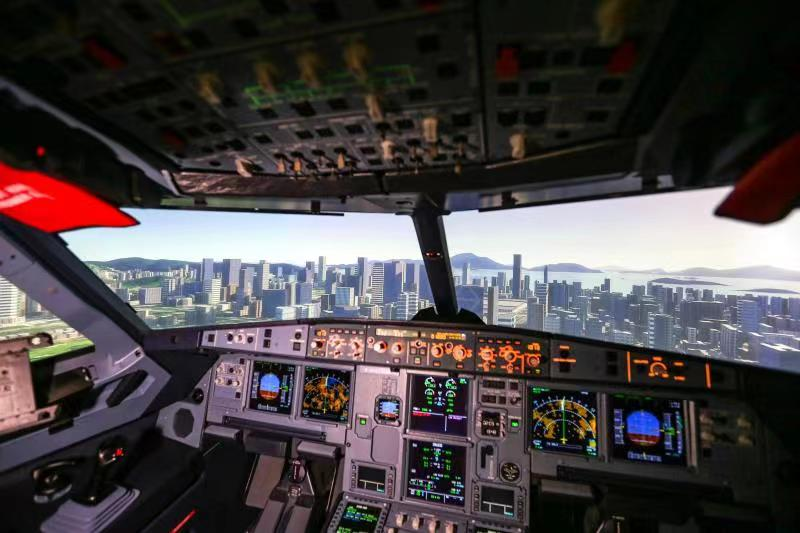
\includegraphics[width=6cm]{pictures/simulator.jpg}
        \caption{D级模拟机内部}
        \label{siminn}
    \end{minipage}
\end{figure}
\par
近年来我国用于飞行员训练的D级模拟机均来自CAE、Flight Safety等国外模拟机制造商。2020年北京蓝天航空科技有限公司研发的新舟60飞机对应的全动模拟机通过了D级飞行模拟机认证,开始打破国外模拟机制造商对于D级飞行模拟机研制的垄断,迈出了国产模拟机的坚实一步\cite{simhis3}。
但新舟60本已是几近停飞的老旧型号飞机,市场存量很小,更复杂的市场主流型号客机以及C919客机模拟机的自主研发仍在进程中。
\subsection{视景系统}
最早的飞行模拟机并不具备视景系统,驾驶员仅能坐在木制机舱中体验旋转。在上世纪30年代,一个位于机身前循环播放的画轴被视为第一个视景系统。60年代闭路电视的发展让视景系统有了新形态,通过相机扫过带有场景的皮带再将画面投影至飞行员眼前作为视景\cite{vishis1},此设备可以模拟简单光照,但仍是二维视觉效果。计算机图像生成技术则将视景系统拉入三维时代,发展至今成为根据飞机位置调取场景数据库,并结合多种环境设置完成渲染的现代视景系统\cite{vishis2}。
\par
目前在视景系统方面,能够参与并通过D级飞行模拟机鉴定的视景系统主要为CAE公司的Tropos视景系统和Flight Safety公司的VITAL视景系统\cite{vishis3},它们都被使用在各公司自研的飞行模拟机上。RSI公司则专注于视景系统开发,其研制的Epic Visual System视景系统已经超过D级标准,对4K分辨率图像实时渲染帧率已能够达到120HZ\cite{simhis4}。
而国内关于视景系统的研究开发还不能通过最高标准的验收,在当前国际背景下,研制出能够搭载于D级飞行模拟机上并通过鉴定的视景系统,对打破垄断突破技术封锁有重要意义。
\par
无论是服务于娱乐休闲还是专业训练,现如今一款视景系统的开发必然要基于基本的图形引擎,综合功能更强大的游戏引擎当然是更好的选择。在游戏引擎出现之前,需要数学、图形、物理等各个领域的专家齐聚一堂花费大量时间精力才能完成一个简单的游戏\cite{engine2}。
游戏引擎则是集合图像渲染引擎、物理引擎、网络引擎、动画引擎、脚本引擎、人工智能引擎等于一身,将功能封装为组件供开发者直接调用,大大降低学习成本,缩短开发周期\cite{engine3}。
目前最主流的商业游戏引擎莫过于EPIC公司的Unreal Engine以及Unity Technologies 公司的Unity3D。它们在技术上集成了各类游戏开发所需引擎,可以实现极高的画面质量,且支持PC、移动端、游戏机等设备,达成多平台兼容,在业界运用程度高范围广\cite{engine1}。
\par
杜等人基于OGRE面向对象图形引擎实现视景渲染\cite{engine5},其主要研究了大地形的渲染算法;董等人依托于视景仿真软件Mantis,设计了针对某军用型号飞机的视景系统\cite{engine4}。
本文中的民航视景系统则是基于腾讯自研游戏引擎CrossEngine开发。
从业界来看,国内外知名游戏厂商基本都有内部自研游戏引擎,且经过几代产品的迭代打磨,在业内已经具有相当的影响力,例如EA公司的Frostbite\cite{crossengine},网易游戏的NeoX和Messiah引擎也已为公司创造了巨大的价值。
近年来受国际关系的影响,使用第三方商业引擎成为了一个潜在的风险,CrossEngine便在此背景下诞生。
使用自研引擎开发视景系统可以更加自由的调整渲染风格,从更底层角度提升渲染效率,助力达成D级模拟机的验收标准。
\section{本文主要工作}
本项目目标是开发能够搭载于D级全动飞行模拟机上的视景系统,本文主要描述该视景系统中数据交换子系统的设计与实现。
该子系统旨在为只使用数据链路层协议的仿真机与使用更高层网络协议的图像生成器间搭建双向沟通的桥梁,是视景系统运作的基础。本文工作主要涉及以下几点:
\begin{itemize}
    \item [(1)]
    在项目开始阶段使用网络抓包工具对进口模拟机的输入输出数据包进行分析,发现其中只有以太网协议头部信息,说明仿真机的网络协议栈相当简单,与基于游戏引擎开发的图像生成器并不在同一层面上。
    为解读数据帧中指令的具体信息,又结合有限的文档信息进行分析,确认了部分指令的数据组织结构与数字表示方法。
    \item [(2)]
    基于上一步中的认知,对视景系统中的数据交换子系统进行了需求分析和设计。其主要的功能要求是按照仿真机的既定规则收发数据帧,将其解析为自定义指令后再与图像生成器交流。
    明确需求的基础上,设计了系统用例,结合逻辑、开发、时序和部署视图确定了系统架构。
    在实现部分完成了确认的21条仿真机控制指令和5条视景系统反馈指令的转换,保障如飞行、天气变化、碰撞检测等基本功能的实现。
    \item [(3)]
    开发完成后,去到飞行训练基地对系统进行测试,测试环境下实现模拟座舱前方球幕的投影需要多个图像生成器融合投影,过程中发现在投影拼接部分会出现肉眼可观察的图像撕裂与跳帧现象。
    问题在于虚拟仿真机接收数据频率的不稳定,以及数据不能同时到达多台图像生成器。本文设计的网络帧缓冲机制可以同时缓解以上两种问题。
    \item [(4)]
    加入帧缓冲机制后再次测试,发现画面之间仍有肉眼可察的抖动现象。排查后发现是多台投影仪刷新时间点不同步导致的问题。
    本系统中利用了实际刷新时间和理论时间的差值对数据进行了插值平滑,减少了图像间的抖动现象。
    \item [(5)]
    基于基础功能并引入两种机制后最终进行测试,飞机可以在仿真机的驱动已基本稳定60帧的条件下飞行,且运行过程中没有出现明显的图像撕裂和抖动问题。

\end{itemize}
\section{本文组织形式}
本文围绕视景系统中数据交换子系统的设计与实现展开论述,共分为六章,每一章的内容编排如下所述:\par
第一章 引言。本章首先阐述了飞行模拟视景系统以及数据交换子系统的背景与项目意义,明确了本文的工作价值。
       之后对于国内外飞行模拟机、视景系统的技术发展历程做了概述,确定了全动飞行模拟机逐步国产化的宏观目标。\par
第二章 相关技术概述。本章对于数据交换子系统中相关的软件和算法做了介绍。软件部分主要介绍了WireShark网络分析工具,WinPcap架构、Tbuspp中间件、CrossEngine游戏引擎;
       算法部分则介绍了ProtoBuffer协议的编码方式,Nagle算法,和垂直同步机制。\par
第三章 基础数据交换的需求分析与概要设计。本章首先阐述了视景系统的运行方式,对进口仿真机的通信机制进行了研究。在此基础上对数据交换子系统进行了需求分析,并确定了系统用例。
       随后结合逻辑视图、开发视图、进程视图和部署视图对子系统的概要设计进行说明。确认了系统的四个模块。\par
第四章 基础数据交换的详细设计与实现。本章在概要设计的基础上,为仿真机侧数据交互模块,数据转换模块,图像生成器侧数据交互模块结合顺序图、类图和时序图阐述了各自的详细设计,并通过解释关键代码说明了三个模块各自的实现细节。\par
       
第五章 数据同步与平滑机制的引入。本章开篇对数据交换系统按照指令代号进行了测试,期间发现存在多投影仪投影帧不一致、图像抖动问题。经问题排查与分析后加入了网络帧缓冲机制,帮助多个图像生成器中的数据同步;引入插值平滑机制抑制抖动问题。\par
第六章 总结与展望。本章对本文中的重点工作进行简要总结,并对目前本视景系统面临的问题及未来的发展方向进行了分析。

\chapter{相关技术概述}

\section{WinPcap架构}
WinPcap(windows packet capture)是由意大利人Loris Degioanni在2000年提出并实现的一个架构,目的在于为Windows平台应用程序提供访问网络底层的能力\cite{winpcap1}。
传统socket通信中,两台主机之间通信,socket接收到的内容都是已经过网络协议栈处理的通信内容,并不会含有如数据帧头,IP头,TCP/UDP等内容。WinPcap功能在于独立于操作系统的网络协议栈而发送和接收数据帧,非常适合做网络协议分析、网络监控等工作\cite{winpcap2}。
\par
抓包系统必须绕过操作系统的协议栈来访问在网络上传输的数据帧,这就要求一部分运行在操作系统核心内部,直接与网卡驱动交互。Winpcap是针对Win平台上的抓包和网络分析的一个架构。它包括一个内核态的包过滤器,一个底层的动态链接库packet.dll和一个用户态的程序接口库wpcap.dll\cite{winpcap3}。
本系统中用其收取和发送数据链路层上的数据帧,帮助视景系统与仿真机交流。
\begin{figure}[h!]
    \begin{center}
        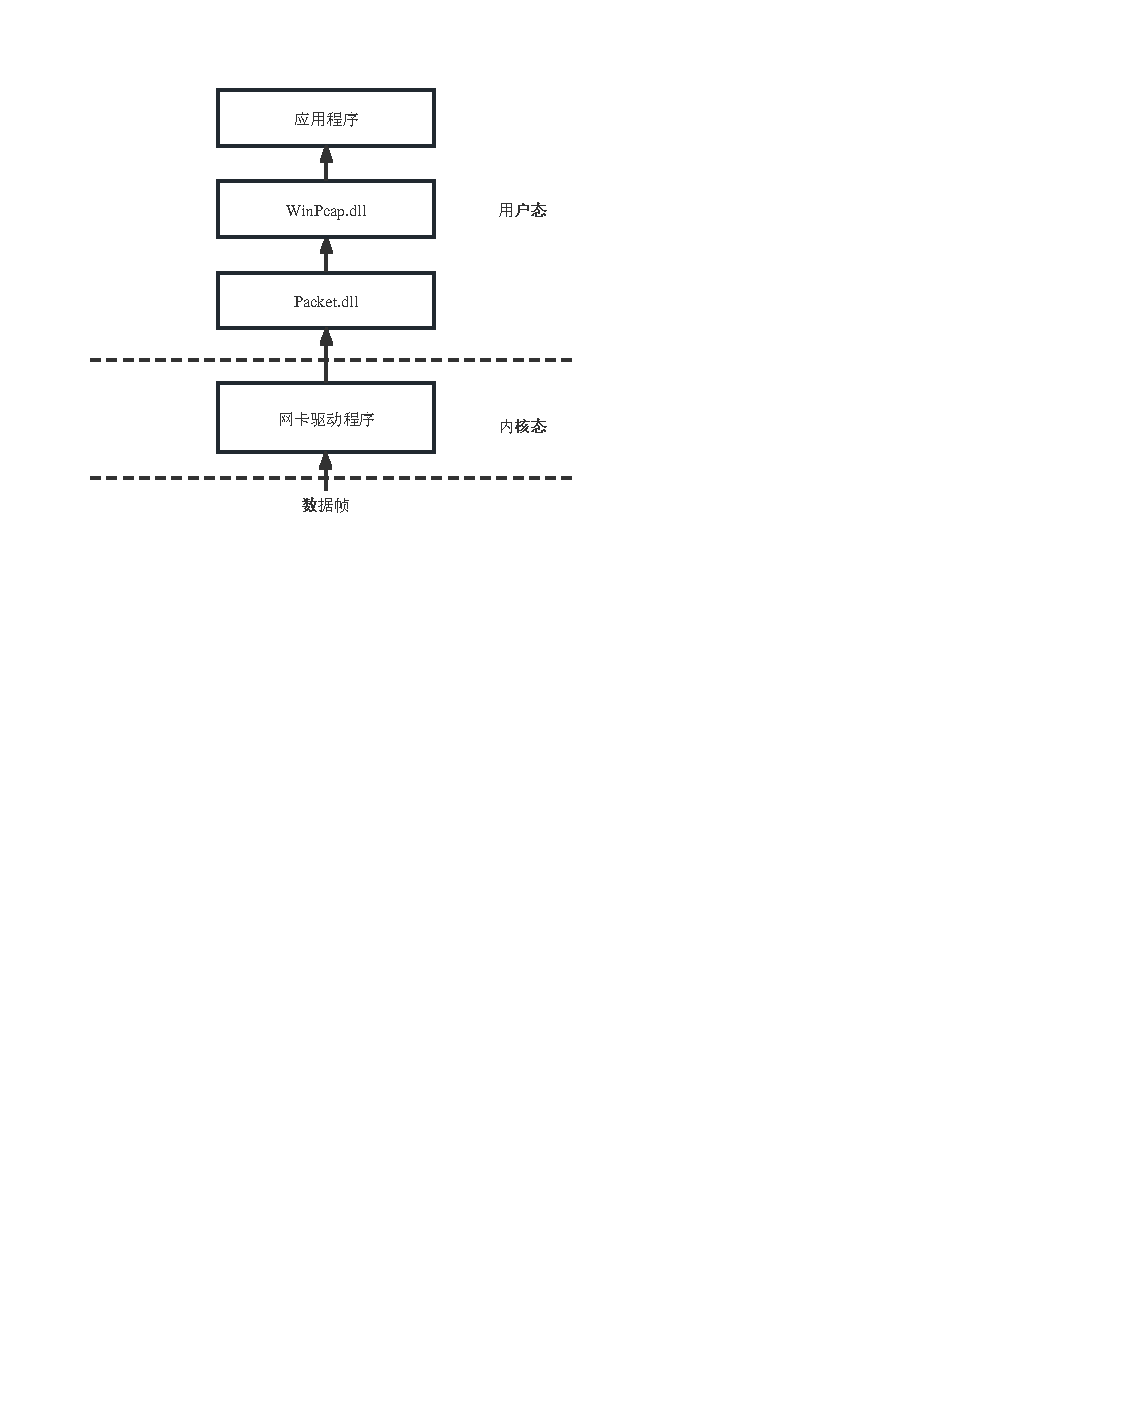
\includegraphics[width=0.6\textwidth]{pictures/winpcap.pdf}
        \caption{WinPcap结构}
        \label{wincapstruc}
    \end{center}
\end{figure}
\section{ProtoBuffer协议}
Protocol Buffer是Google提供的一种数据序列化协议,可用于通讯协议、数据存储等领域的语言无关、平台无关、可扩展的序列化结构数据格式\cite{Protobuf1}。它属于一种二进制协议,相比较文本协议如XML,JSON等在体积和封解包速度方面有巨大的优势\cite{Protobuf2},适合诸如本系统的实时渲染应用。
\par
ProtoBuffer序列化后消息紧凑得益于巧妙设计的编码方式。
首先其使用了Varint这种紧凑的表示数字的方法。它用一个或多个字节来表示一个数字,值越小的数字使用越少的字节数。这能减少用来表示数字的字节数。
Varint中的每个字节的最高位有特殊的含义,如果该位为1,表示后续的字节也是该数字的一部分,如果该位为0则结束,其他的7位都用来表示数字,因此小于128的数字都可以用一个字节表示,而不是统一为4个字节。
从统计的角度来说,一般不会所有的消息中的数字都是大数,大多情况下采用Varint可以用更少的字节数来表示数字信息。在进一步的优化中使用到了ZigZag编码,即用无符号数交错表示正数与负数,减少了负数的编码长度。
\par
其次ProtoBuffer对Key的定义为field\_number+wire\_type,field\_number表示该属性在结构中的编号,3位的wire\_type则指明了该属性的类型。
ProtoBuffer中共有6种wire\_type,如表\ref{pbtype}所示。
\begin{table}[h!]
    \begin{center}
        \caption{ProtoBuffer类型列表}
        \label{pbtype}
        \renewcommand\arraystretch{1.5}
        \begin{tabularx}{0.8\textwidth}{ 
            | >{\centering\arraybackslash\hsize=.5\hsize\linewidth=\hsize}X 
            | >{\centering\arraybackslash\hsize=.5\hsize\linewidth=\hsize}X 
            | >{\centering\arraybackslash\hsize=\hsize\linewidth=\hsize}X 
            | }
            \hline
            \textbf{ID} & \textbf{名称} & \textbf{包含类型}\\
            \hline
            0 & VARINT & int32, int64, uint32, uint64, sint32, sint64, bool, enum\\
            \hline
            1 & I64 & fixed64, sfixed64, double\\
            \hline
            2 & LEN & fixed64, sfixed64, double\\
            \hline
            3 & SGROUP & group start (deprecated)\\
            \hline
            4 & EGROUP & group end (deprecated)\\
            \hline
            5 & I32 & fixed32, sfixed32, float\\
            \hline
        \end{tabularx}
    \end{center}
\end{table}

\par
解包过程中XML需要从文件中读取出字符串,再转换为XML文档对象结构模型。之后再从XML文档对象结构模型中读取指定节点的字符串,最后再将这个字符串转换成指定类型的变量。其中的计算消耗无疑非常巨大。
ProtoBuffer在解包时只需要简单地将一个二进制序列,按照指定的格式读取到对应的结构体中就可以了。当然这也说明其必须要事先编写结构体文件给到接收方,否则无法正确解包。
\section{Tbuspp中间件}
Tbuspp是腾讯为完整解决游戏后台复杂与低延迟通讯需求而建立的服务网格中间件。
随着分布式架构越来越复杂和服务越拆越细,开发人员迫切的希望有一个统一的控制面维护和管理各项服务。边车模式有效分离了系统控制和业务逻辑,使开发人员专注业务逻辑\cite{tbus2}。
服务网格是用于处理服务间通信的基础设施层,服务可以插入其中的代理网格,代理作为边车注入到每个服务部署中\cite{tbus1}。服务间的调用通过代理实现,封装了其复杂性。
\par
Tbuspp的目标是构建功能完备的面向消息通讯中间件,能够完整解决全球同服部署模式下,游戏后台复杂与低延迟通讯需求,并能尽量降低开发与运维成本,做到简单易用。
其与Envoy等流行的开源服务网格组件有两点本质区别,第一是提供专用API供应用服务调用,与Envoy采用透明方式劫持应用服务的流量存在显著差异。
第二是基于SHM消息队列与应用服务交换消息,这点是针对游戏服务特殊的业务背景:游戏服务一般是有状态服务,希望在对服务快速重启更新的同时,保持游戏世界状态的连续性,因此往往需要将核心运行状态保存在SHM中,同时也基于SHM与边车交换消息,以便服务重启期间不间断消息收发。
本系统中使用Tbuspp作为虚拟仿真机与游戏引擎间进行TCP消息沟通的插件。
\section{Nagle算法}
在使用一些协议通讯时,如果每次只发送一个字节的有用信息,却要附带几十个字节的头部信息,这笔开销会增加拥塞情况的出现。
John Nagle就提出了一种通过减少需要通过网络发送包的数量来提高TCP/IP传输的效率\cite{nagle2},即Nagle算法。
Nagle算法核心是避免发送小的数据包,要求一个TCP连接上最多只能有一个未被确认的小分组,在该分组的确认到达之前不能发送其他的小分组。TCP会搜集这些小的分组,然后在之前小分组的确认到达后将刚才搜集的小分组合并发送出去。
\par
但Nagle算法也有弊端,对于实时性要求很高的交互上,我们不能使用Nagle算法\cite{nagle1}。
比如在网络游戏中,每一帧玩家的操作信息或状态改变并不会产生很大的包体,却需要及时的将状态同步到服务器中。此时若Nagle算法启用,部分信息将被延迟给到服务端,严重影响用户体验。
因此特别是在一些对时延要求较高的交互式操作环境中,必须禁用Nagle算法,让所有的小分组必须尽快发送出去。

\section{CrossEngine游戏引擎}
游戏引擎是打造出优秀游戏的核心因素之一,CrossEngine是腾讯为降低商业风险提升核心能力而自研的跨平台游戏引擎。其基础架构参考了ECS框架,
这是一种主要用于游戏引擎的软件开发架构,大体上由实体Entity、组件Component和系统System三部分构成\cite{ce1}。其中实体是对场景内需要逻辑控制的物体的抽象;组件代表被挂载于实体上的数据,一个实体可以搭载若干组件,相当于该实体被赋予了一系列属性;系统在此架构中承担了全部的逻辑代码,可以访问实体中的组件。
此架构突出了组合大于继承的理念,可以更加灵活的表示现实甚至想象出的概念。引擎中如内存分配、数学运算、资源管理等核心基本由C++编写,引擎编辑器主要由C\#开发。图\ref{ceeditor}展示了目前CrossEngine的编辑器界面。
\begin{figure}[h!]
    \begin{center}
        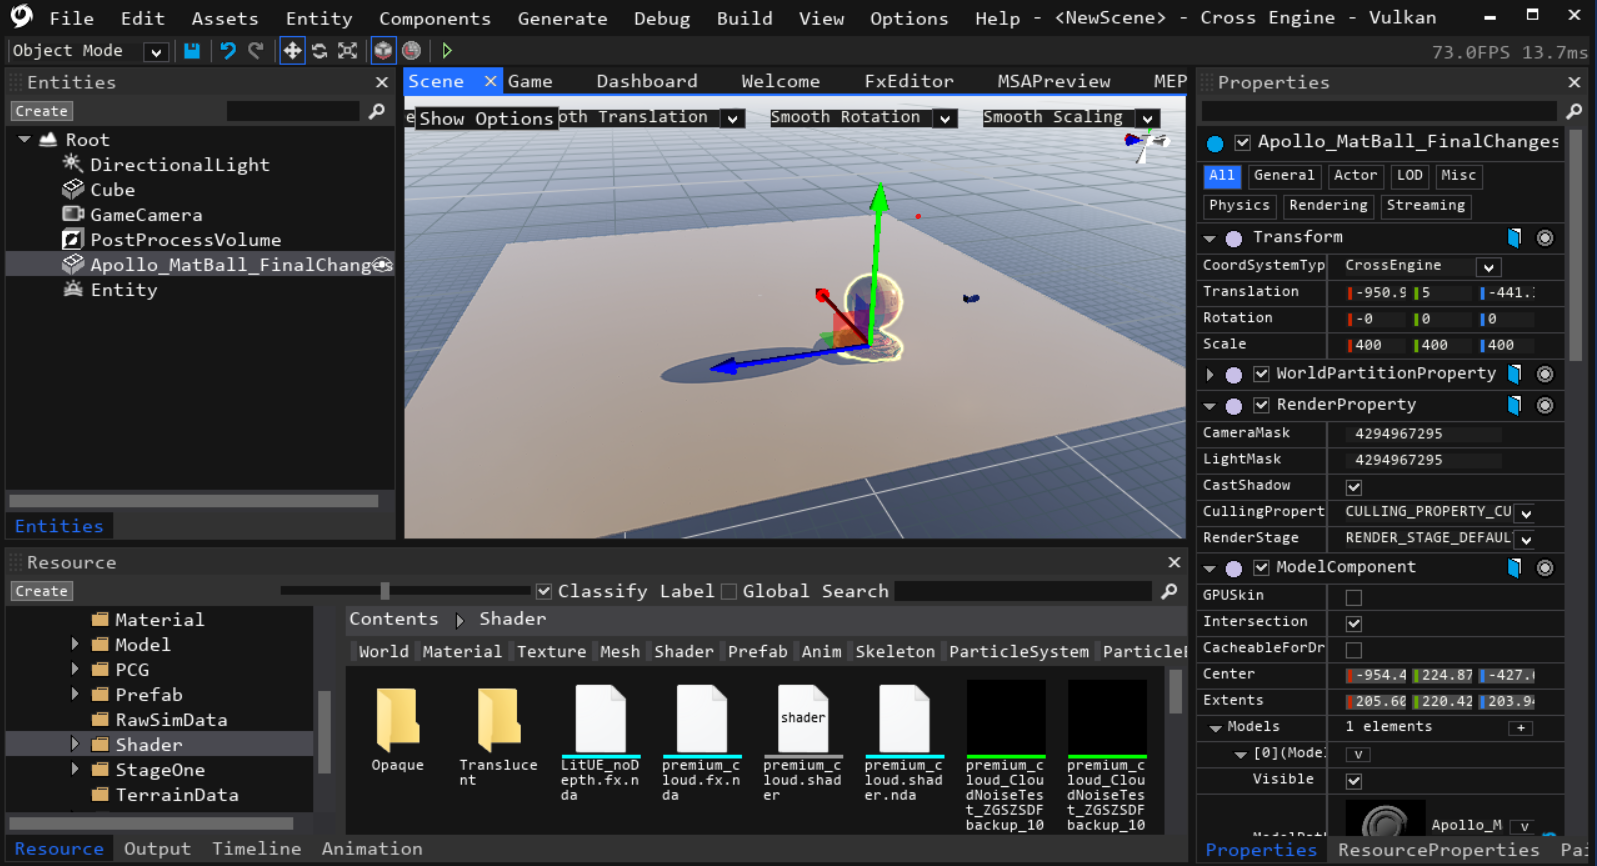
\includegraphics[width=0.9\textwidth]{pictures/crossengine.png}
        \caption{CrossEngine编辑器}
        \label{ceeditor}
    \end{center}
\end{figure}
\par
目前CrossEngine引擎已具备一定程度的生产实践能力。渲染方面目前已支持DX12、Vulkan、GLES3渲染后端,HDR-LinearSpace工作流内置基于物理的渲染;
功能系统方面具备基于PhysX的物理引擎,骨骼动画系统、粒子系统、脚本系统也基本完善。编辑器部分则是对标商业引擎主流设计,尽可能降低学习成本。
CrossEngine从最初的架构设计到三方基础库的选型都为Runtime尺寸做了许多工作,如表\ref{enginert}所示在该方面对比商业引擎有一定优势。在后续开发中也将坚持控制Runtime在较小的尺寸,以带来更多应用可能。
\begin{table}[h!]
    \begin{center}
        \caption{引擎Runtime比较}
        \label{enginert}
        \renewcommand\arraystretch{1.5}
        \begin{tabularx}{0.8\textwidth}{ 
            | >{\centering\arraybackslash\hsize=.5\hsize\linewidth=\hsize}X 
            | >{\centering\arraybackslash\hsize=.5\hsize\linewidth=\hsize}X 
            | }
            \hline
            \textbf{游戏引擎} & \textbf{Runtime体积} \\
            \hline
            CrossEngine & 2.2m \\
            \hline
            UnrealEngine4 & 40m+\\
            \hline
            Unity & 23m\\
            \hline
        \end{tabularx}
    \end{center}
\end{table}

% \section{Lua脚本}
% Lua 是一种用标准C语言编写而成的轻量级嵌入式脚本语言,其设计目的是为了嵌入应用程序中,从而根据不断变化的需求为应用程序提供灵活的扩展和定制功能\cite{Lua}。
% 不同于更广为人知的Python脚本,Lua诞生时的定位决定它并没有提供强大的库,所以Lua并不适合作为开发独立应用程序的语言,更多是调用宿主语言如C++中提供的核心方法以实现逻辑。因此Lua被广泛应用在游戏逻辑开发、openwrt系统中与宿主语言结合。
% 著名游戏《魔兽世界》中的客户端逻辑便是使用Lua编写。

% \par
% Lua作为解释性语言不需要编译过程,有更强的跨平台能力,且节省了开发过程中对于逻辑代码反复修改的编译时间,总之可以更灵活地应对各方面变动。本系统中用于观察系统效果和生成反馈信息的飞机飞行逻辑便是通过Lua脚本实现,其中调用如物体旋转、射线发射等游戏引擎中C++编写的方法,尽可能避免引擎核心的改动。
\section{WireShark抓包工具}
\section{帧缓冲机制}
\section{插值算法}
\section{航空坐标系及坐标系转换}
在模拟飞行中,涉及到位置和旋转的数据都是以某个坐标系为基础,常用坐标系有飞机自身坐标系、经纬高LLA坐标系、地心地固ECEF坐标系和北东天ENU坐标系。
其中只有LLA坐标系是以经度纬度海拔确认位置的坐标系,其余均为笛卡尔坐标系。
\begin{itemize}
    \item [(1)]
    飞机自身坐标系一般以驾驶舱位置为原点O,Z轴指向飞机下方,X轴指向飞机左侧,Y轴垂直于xOz平面指向飞机前方构成右手坐标系,如图\ref{crood1}所示。
    其作用为确定飞机上如起落架、各类灯的相对位置\cite{crood4}。
    \begin{figure}[h!]
        \begin{center}
            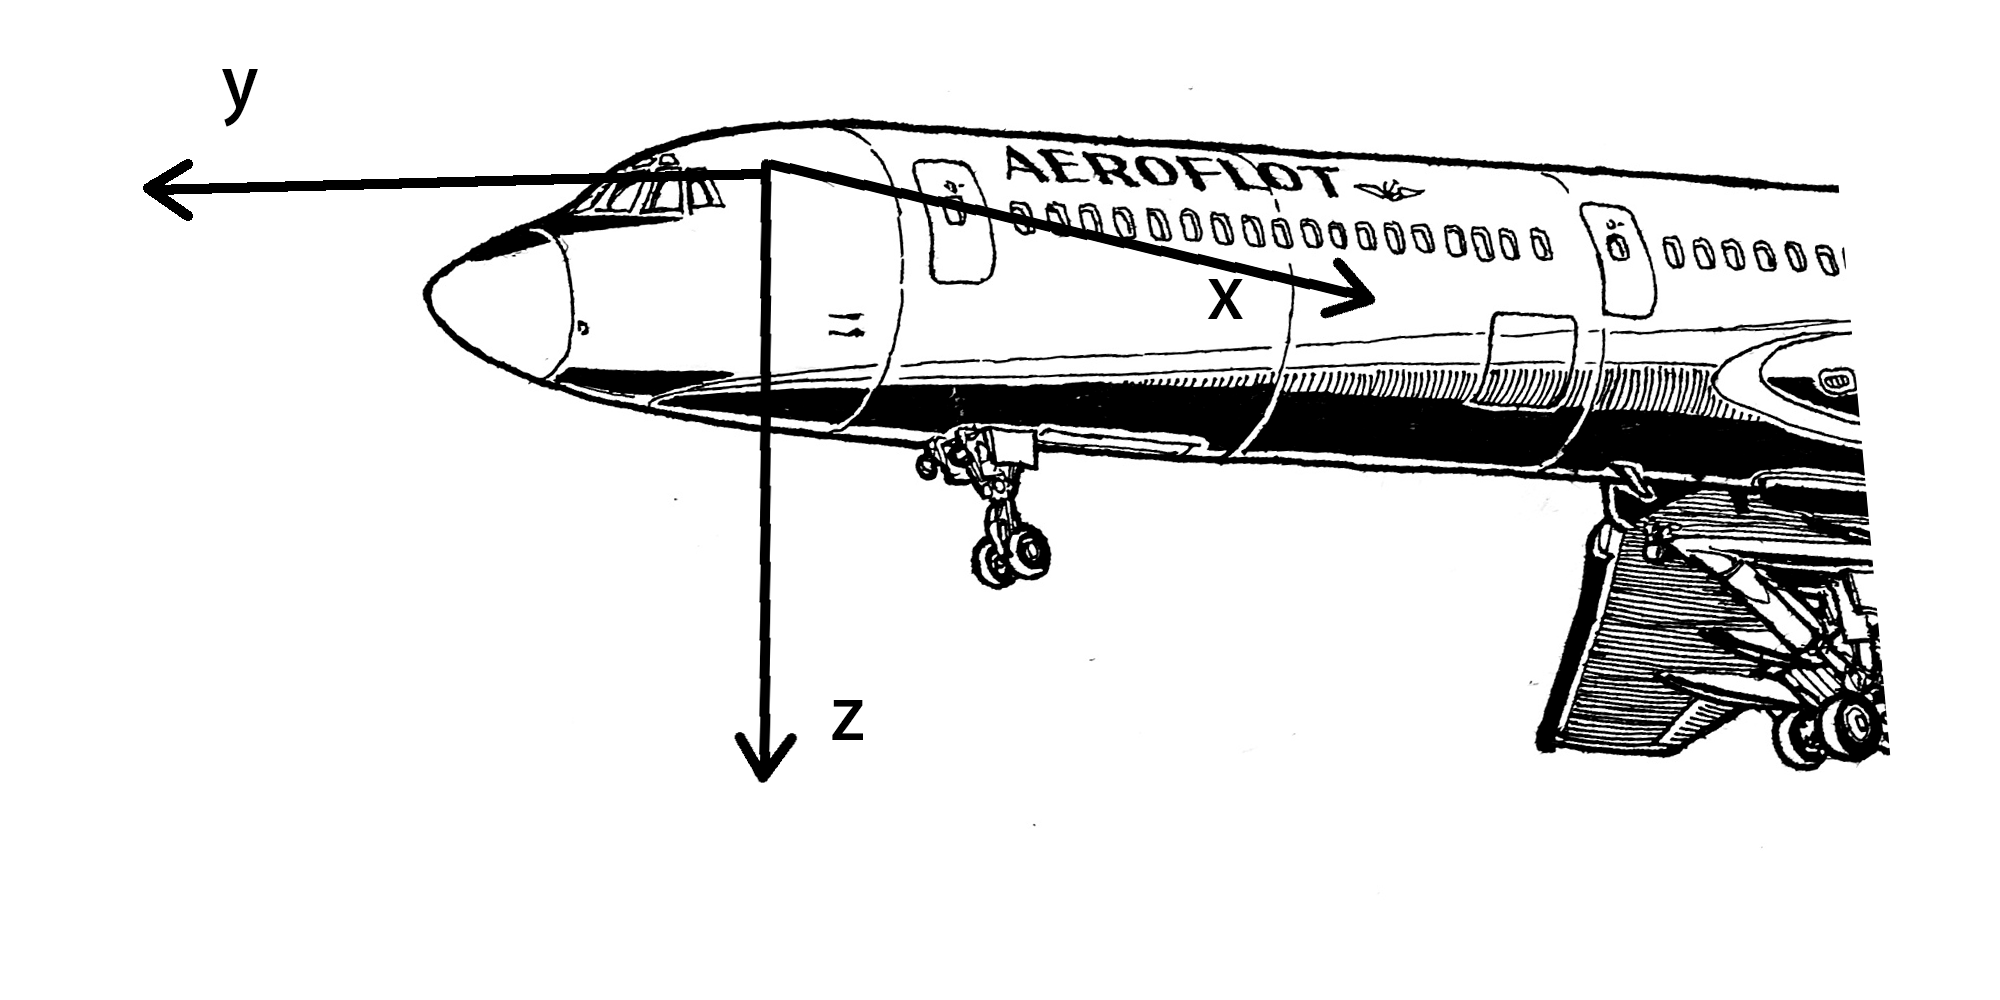
\includegraphics[width=0.8\textwidth]{pictures/plane.png}
            \caption{飞机自身坐标}
            \label{crood1}
        \end{center}
    \end{figure}
    \item [(2)]
    LLA坐标系是以经度纬度海拔来确定位置的球面坐标系。对地球而言经度的定义为本初子午线为0经度,向东增加。
    纬度的定义为椭球表面的法线与赤道面的夹角角度。海拔则是沿椭球表面法线方向距离平均海准面的距离。地球的形状则是以WGS-84为准,地球为长半轴6378137.0米,扁率1/298.257223563的椭球\cite{crood1}。
    在FFS中,仿真机给出的飞机位置信息便是经纬高的形式。
    \item [(3)]
    地心地固坐标系ECEF是一种以地心为原点的地固坐标系。原点O(0,0,0)为地球质心,Z轴与地轴平行指向北极点,X轴指向本初子午线与赤道的交点,Y轴垂直于xOz平面构成右手坐标系\cite{crood2}。
    在视景系统中需要以该坐标系作为世界坐标系,即所有物体的坐标最终都要转换到该坐标系下。
    \item [(4)]
    东北天ENU坐标系是以物体所在球面位置为原点,X轴指向东方,Y轴指向北方,Z轴垂直于xOy面指向天空构成的右手坐标系\cite{crood3}。
    在FFS中,每一帧下飞机的初始姿态便是在该坐标系下,且飞机的旋转是以偏航Yaw,俯仰Pitch,翻滚Roll的顺序完成。
    \begin{figure}[h!]
        \begin{center}
            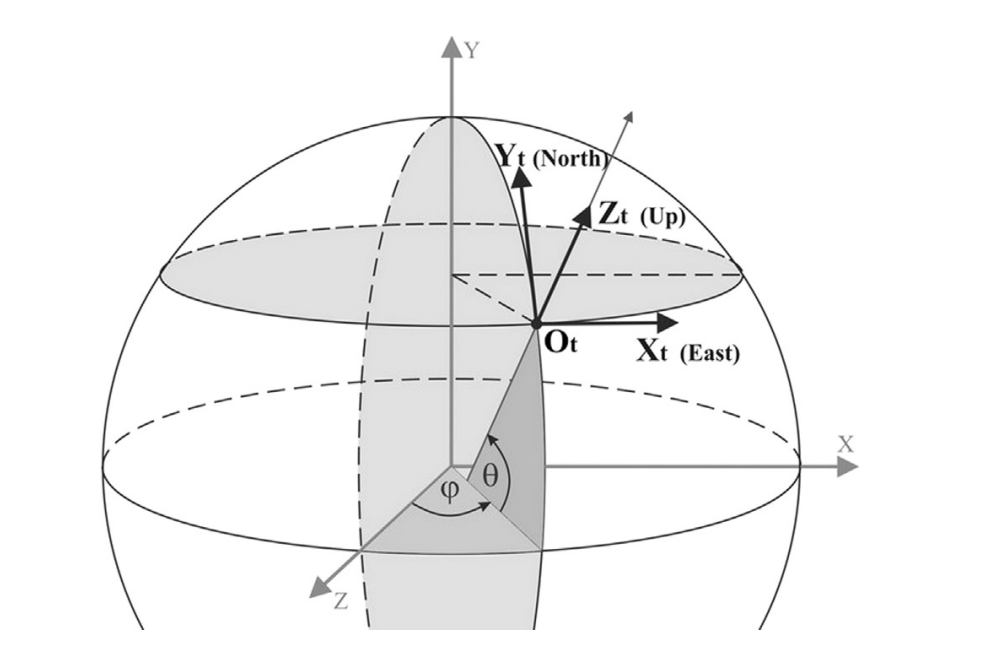
\includegraphics[width=0.8\textwidth]{pictures/coord.png}
            \caption{三类坐标系}
            \label{crood2}
        \end{center}
    \end{figure}
\end{itemize}
\par
以上是航空常用4种坐标系,在实际需求中必然涉及飞机的旋转以及坐标在不同坐标系下的变换。
向量的旋转和坐标的变换可以通过旋转矩阵完成\cite{rotate1}。最直观的旋转操作是按照固定坐标轴依次旋转,在三维空间中,按z轴旋转$\alpha$角度可以表示为如下形式。
旋转矩阵中的列向量为旋转后坐标系的坐标轴在旋转前的坐标系中的坐标,自然互相正交且为单位向量,所以旋转矩阵为正交矩阵。旋转的逆变换可以直接使用转置矩阵作为逆矩阵。
~\\

\begin{math} 
    \begin{gathered}
        \begin{bmatrix} p_x' \\ p_y' \\ p_z'\end{bmatrix} 
        \quad 
        =
        \quad
        \begin{bmatrix} 
            cos(α) & -sin(α) & 0 \\
            sin(α) & cos(α) & 0 \\ 
            0 & 0 & 1
        \end{bmatrix}
        \quad
        \begin{bmatrix} p_x\\ p_y \\ p_z \end{bmatrix}
    \end{gathered}
\end{math}

~\\
\par
坐标系的转换也可视为旋转,特别要注意,上述公式中矩阵的意义是将如图\ref{crood3}中p点在旋转后的坐标系(红色)中的坐标,转换为旋转前的坐标系(黑色)中的坐标。
此时将旋转矩阵中的列向量视作旋转后坐标轴在旋转前坐标轴上的投影,或者叫做方向余弦。

\begin{figure}[h!]
    \begin{center}
        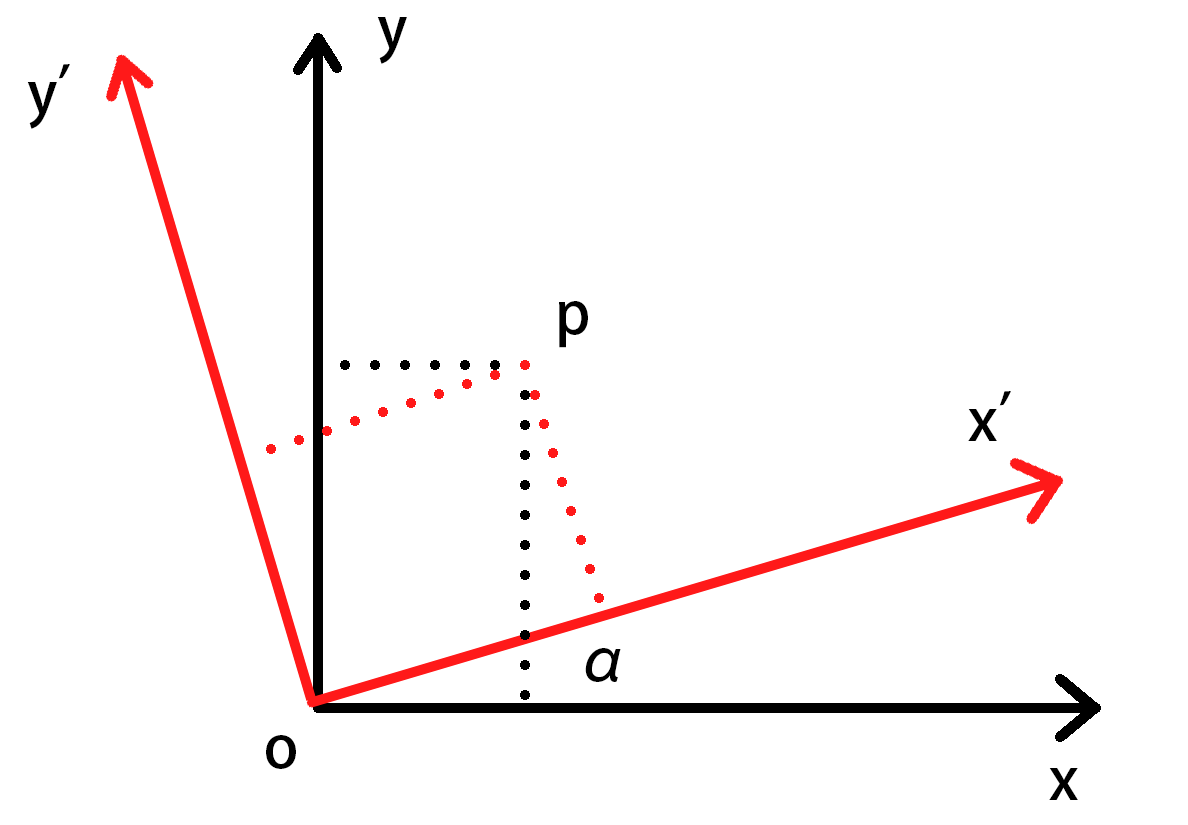
\includegraphics[width=0.6\textwidth]{pictures/rotate.png}
        \caption{坐标系变换}
        \label{crood3}
    \end{center}
\end{figure}
\par 
旋转在游戏引擎中都是通过四元数进行。上文中提到的按照坐标系轴依次旋转的方式,旋转轴顺序的变换会影响最终结果,且旋转时不幸让某些坐标轴重合了就会发生万向节死锁,
导致丢失一个方向上的旋转能力\cite{rotate3},始终得不到最终结果。四元数可以简单理解为一个任意旋转轴加旋转角度,对人类而言直观性会下降,但能够减少矩阵计算的复杂度,还可以方便的进行插值操作\cite{rotate2}。
\section{本章小结}
本章介绍了视景系统中数据交换子系统开发中涉及的主要技术。。
首先介绍了在数据交换过程中使用到的技术,包括负责绕过OS的网络协议栈直接与网卡驱动交流的WinPcap,具有高序列化与反序列化效率的ProtoBuffer协议,有可能造成小数据包发送延迟的Nagle算法,
以及主要服务于游戏的低延迟通信插件Tbuspp。
其次,介绍了开发本视景系统使用的自研游戏引擎CrossEngine和适合于编写游戏逻辑的嵌入式脚本语言Lua。
最后介绍了模拟飞行中用到的4种航空坐标系,以及计算机中实现旋转和坐标系转换的方式。


\chapter{基础数据交换的分析设计与实现}
\section{全动飞行模拟机整体概述}

\begin{figure}[h]
    \begin{center}
        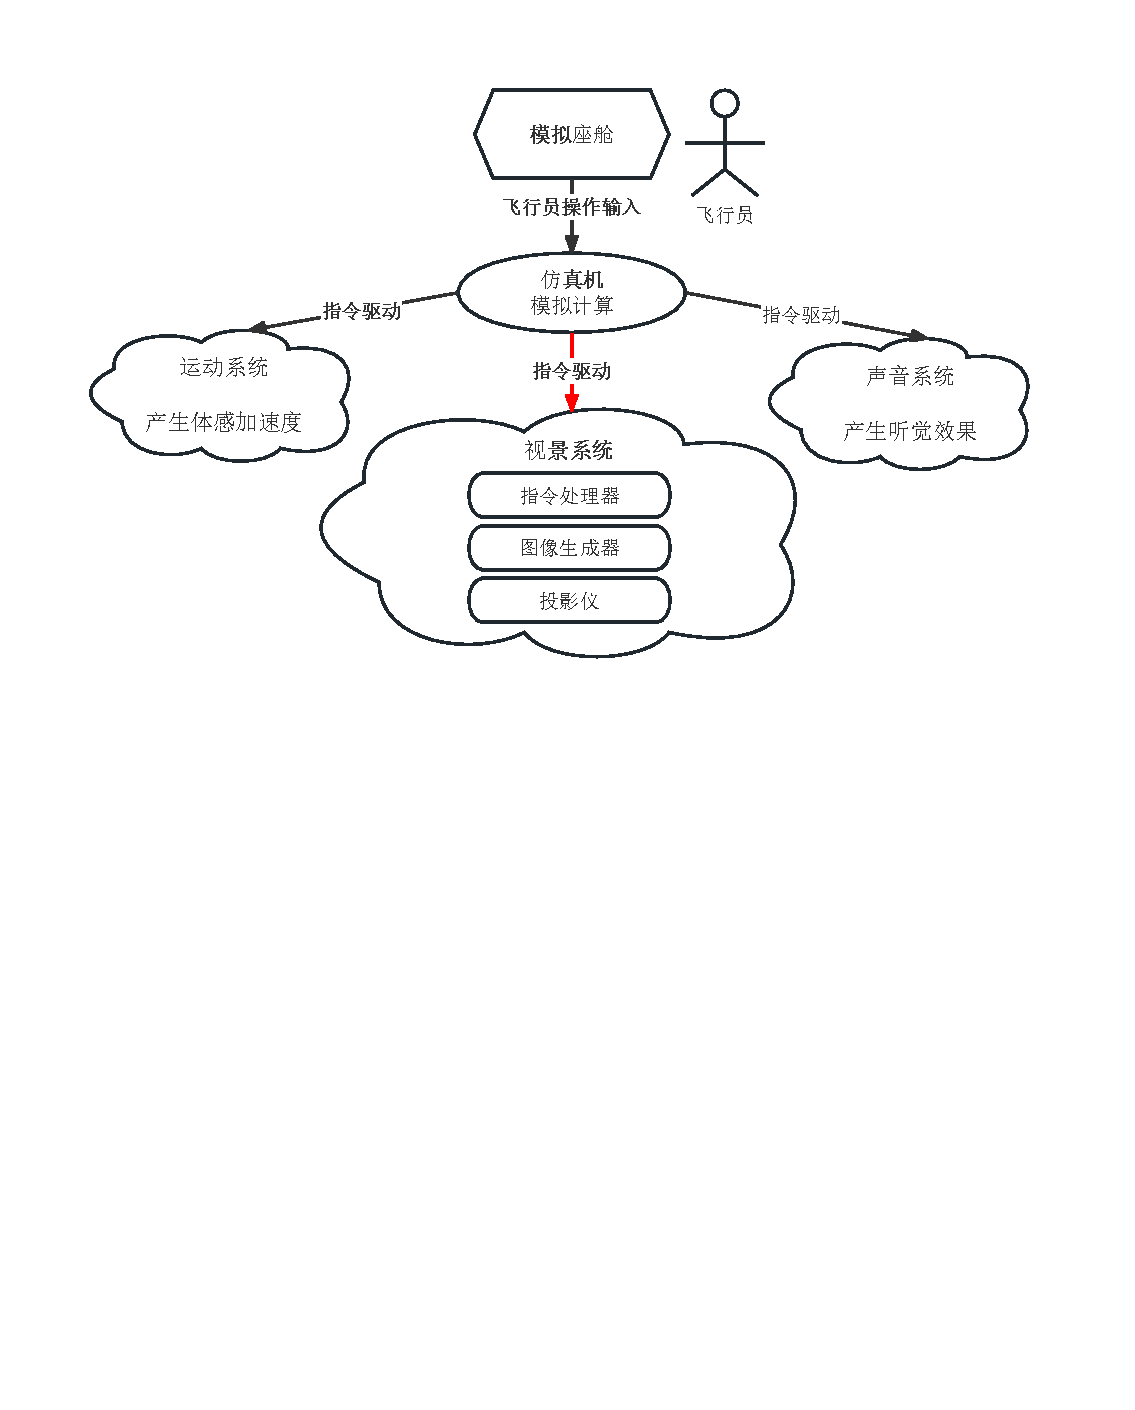
\includegraphics[width=\textwidth]{pictures/simstruct.pdf}
        \caption{模拟机运转方式}
        \label{framework}
    \end{center}
\end{figure}
\section{视景系统整体概述}
视景系统是FFS中负责连续生成模拟座舱前方飞行画面的系统。飞行员在模拟座舱中的操作将作为仿真机的输入,经过模拟计算后输出如位置、姿态、灯光等一系列指令,图像生成器根据指令要求执行逻辑后便可渲染连贯的飞行画面,提供模拟飞行的视觉效果。
同时图像生成器也要以指令的形式反馈给仿真机如碰撞等信息。仿真机可以据此通知如声音、运动系统做出相应反馈。
\par
由上述可知仿真机相当于FFS的服务端,视景系统类似客户端,但此案例的服务端与客户端在网络体系结构中处于不同层级,需要请一个翻译才能正常进行数据交换,本系统中将该翻译角色称为虚拟仿真机。
视景系统整体架构如图\ref{framework}所示。仿真机作为一个底层网络设备,其只能接收或发送仅用以太网协议封装的数据包,且使用该公司自定义的数据交换协议;虚拟仿真机作为翻译需要对双方的消息解封、转换再封装,最后发送。同时在没有仿真机的开发环境下也可以读取模拟数据实现流程;
虚拟仿真机与客户端之间使用ProtoBuffer作为数据交换协议,TCP通信任务由Tbuspp插件承担。图像生成器需要根据收到的指令先完成数据同步工作,再执行逻辑,计算反馈信息。图中虚线框中的部分包含了数据由仿真机到图像生成器中被使用,生成的反馈信息再最终回到仿真机的全过程,此部分便是视景系统中的数据交换子系统。
\par
图像生成器中还含有许多重要的功能组成部分。首先引擎核心为其提供了渲染、物理、脚本、数学计算等运行核心组件,许多逻辑依赖其中的方法实现,逻辑执行结束后也需要渲染介入。
机场资产则是场景的数据库,地形、建筑、纹理等资源皆存于其中,需要根据飞机所处位置去查找并加载这些资源,这对于数据的组织形式,查找策略都有较高的要求。
投影同步插件负责在FFS上运行时控制多台投影仪投影相同的一帧以减少画面撕裂,另外由于模拟座舱前方是一个球幕,需要校准球幕投影时发生的畸变。

\begin{figure}[h]
    \begin{center}
        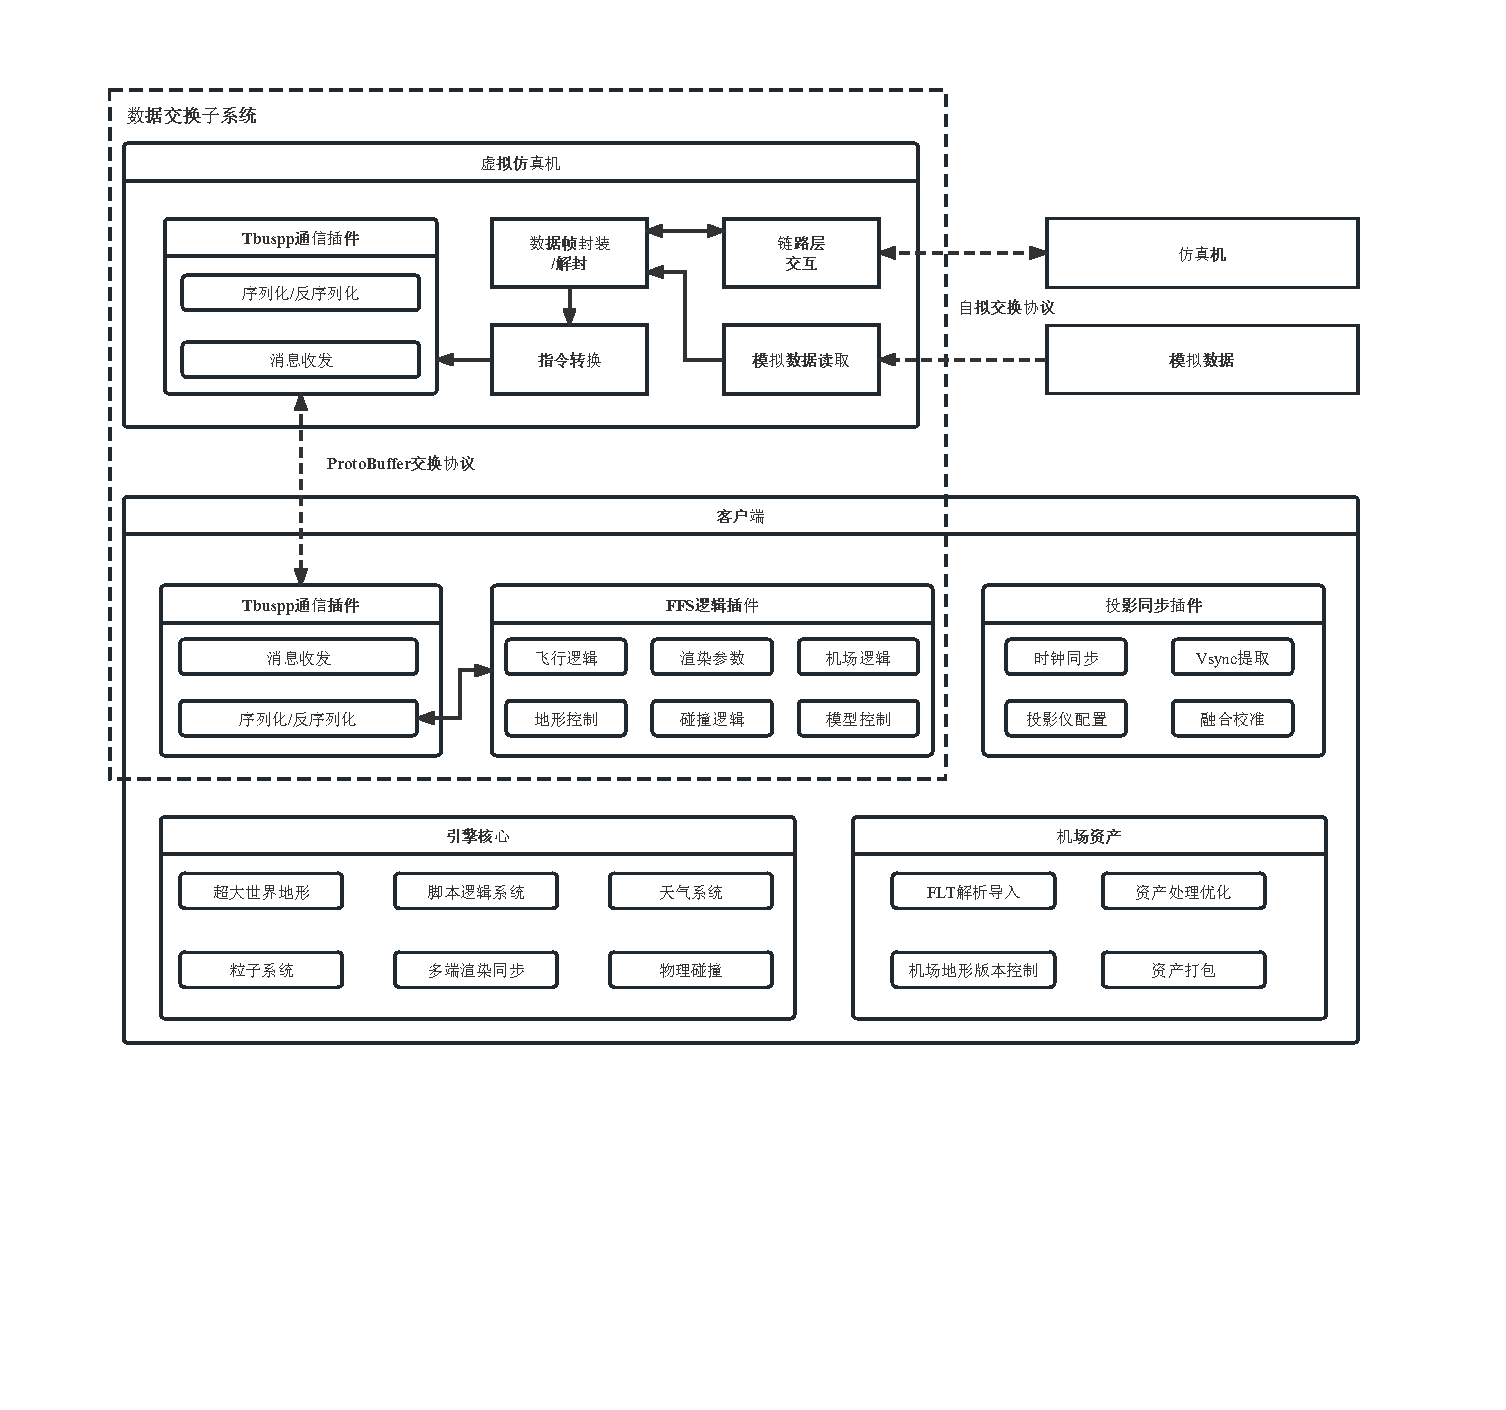
\includegraphics[width=\textwidth]{pictures/sketch.pdf}
        \caption{视景系统整体架构}
        \label{framework}
    \end{center}
\end{figure}
\section{仿真机数据帧分析}

\section{数据交换子系统需求分析}
系统设计的第步是需求分析,其主要目的是明晰用户非形式化
的需求,最终产生完整的需求规格说明。本节首先分析了系统的重点涉众,阐述了涉众对系统的期望。
随后从系统的角度解释软件,定义了系统的功能性需求和非功能性需求。
最后在明确需求的基础上,将各需求拆解为用例,使用用例图和用例描述表详细描述各个用例。
\subsection{涉众分析}
本系统作为视景系统中负责数据交换的子系统,仅包含虚拟仿真机和
图像生成器两个角色。虚拟仿真机作为桥梁希望与仿真机和图像生成器双向交流,而图像生成器希望以稳定的数据驱动逻辑运行。
详细的涉众分析如表\ref{stakeholder}所示。
\begin{table}[h!]
    \begin{center}
        \caption{涉众分析列表}
        \label{stakeholder}
        \renewcommand\arraystretch{1.5}
        \begin{tabularx}{\textwidth}{ 
            | >{\centering\arraybackslash\hsize=.25\hsize\linewidth=\hsize}X 
            | >{\raggedright\arraybackslash\hsize=.75\hsize\linewidth=\hsize}X 
            | }
            \hline
            \textbf{涉众名称} & \textbf{涉众期望}\\
            \hline
            虚拟仿真机 &  作为仿真机与图像生成器间的桥梁,虚拟仿真机希望能正确解释并转换双发发送的指令,
                         能按照仿真机的运行频率及时读取数据并及时发送给图像生成器。同时作为视景系统的一部分,能够屏蔽不同仿真机数据组织结构的差异。\\
            \hline
            图像生成器 &  图像生成器作为执行逻辑和渲染画面的角色,希望从虚拟仿真机处得到数据驱动逻辑执行。
                          另由于多台图像生成器需要同时工作,希望能同时使用基本一致的数据进行运算,最终的融合投影才不会产生撕裂\\
            \hline
        \end{tabularx}
    \end{center}
\end{table}
\subsection{功能性需求}
图像生成器依据仿真机指令进行飞行画面渲染并反馈飞行数据要求仿真机与图像生成器之间进行双向数据交换。如图\ref{netlayer}所示,仿真机作为底层设备其输出与输入均为只用以太网协议封装的数据帧,想要与其沟通必须先结合相关设计文档并进行抓包确认数据帧的数据组织结构和数字表示方法。
掌握规则后便要据此转换指令数据,并按照传统网络体系重新层层封装为便于图像生成器使用的数据段。
因此数据交换子系统中需要一个桥梁角色与建立起仿真机与视景系统的交流,即虚拟仿真机。其同时承担着在没有仿真机的开发条件下读取模拟数据驱动视景运转的责任。
在信息的传输过程中避免不了存在网络波动;且虚拟仿真机与图像生成器间用无法广播的TCP协议通信,对于单一图像生成器而言数据到达频率可能不稳定,对于多个图像生成器而言同一数据到达时刻也不相同。
因此需要进行数据同步抵消差异。另外从单一图像生成器角度,逻辑帧的开始时间受渲染帧约束,不能保证绝对稳定,如果按照仿真机的原始数据飞行可能会产生不自然的闯动,需要一定的数据平滑策略减少影响。
在本视景系统中数据的流动可用下面这一完整流程描述:
\begin{itemize}
    \item [(1)]
    仿真机根据飞行员的输入计算飞行状态,产生一条条指令数据,将这些指令数据仅通过以太网协议封装后以数据链路层数据帧的形式输出。
    \item [(2)]
    虚拟仿真机接收数据链路层数据帧,去除以太网协议的头尾内容,完成解封。识别指令代号后,根据对应数据组织结构直接使用结构体反序列化指令内容。
    \item [(3)]
    将指令中特殊数字表示方式下的数据通过算法转换为常规认知下的数字形式。如将经度0000007f ffffffff转换为179.99后,再赋值给ProtoBuffer结构化数据(也称作message)中的对应字段,生成我们自定义的指令集。
    \item [(4)]
    将该结构化数据通过ProtoBuffer协议进行序列化,并通过TCP协议发送给图像生成器,此过程中的协议封装则全权交由操作系统的内核网络协议栈完成。
    \item [(5)]
    图像生成器接收到数据后,同样由内核网络协议栈解封,再通过ProtoBuffer协议进行反序列化得到指令结构化数据,经过数据同步和平滑后供给逻辑线程使用。
    \item [(6)]
    逻辑线程的反馈信息则通过完全相反的过程,最终逆向发送到仿真机。
\end{itemize}

\begin{figure}[h]
    \begin{center}
        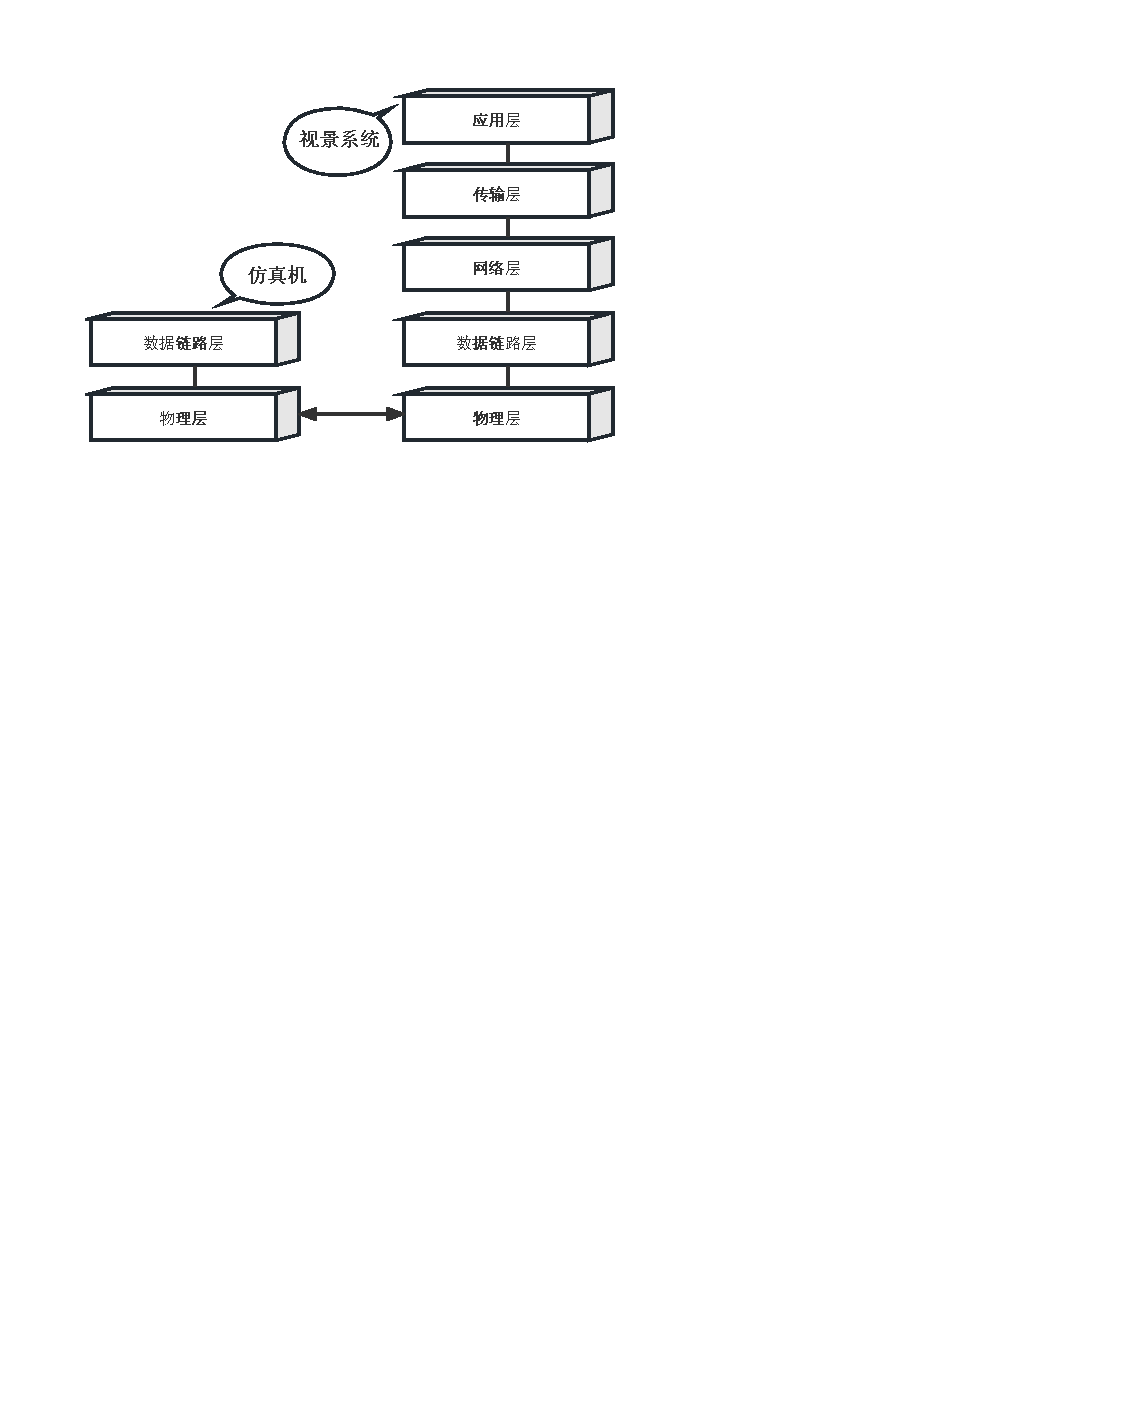
\includegraphics[width=.8\textwidth]{pictures/netlayer.pdf}
        \caption{仿真机与图像生成器层级差异}
        \label{netlayer}
    \end{center}
\end{figure}
\par
% 另外数据交换子系统作为视景系统的一部分,流经它的数据最终要服务于视景系统中的部分逻辑,且反馈数据也来自于逻辑执行。
% 但项目初始阶段视景系统中并不存在任何运行逻辑,因此我们将飞行模拟最基础的飞机飞行一系列逻辑作为数据交换子系统的部分功能。它将使用接收到的指令完成飞行,并将检测到的地形信息作为反馈。
% 最终飞行画面是否正确、流畅也是判断数据交换子系统是否正常运作的重要依据。
整个指令数据传输的过程中需要保证虚拟仿真机与图像生成器依照仿真机的工作频率运行,即数据到达便要处理并发送,这个过程中有一些缓存机制需要禁用。
另外为观察整套数据传输、同步、平滑的效果,需要简单的飞机飞行逻辑观察飞行中画面的效果。
数据交换子系统的功能性需求列表如表\ref{funcreq}所示。
\begin{table}[h!]
    \begin{center}
        \caption{系统功能性需求列表}
        \label{funcreq}
        \renewcommand\arraystretch{1.5}
        \begin{tabularx}{\textwidth}{ 
            | >{\centering\arraybackslash\hsize=.1\hsize\linewidth=\hsize}X 
            | >{\centering\arraybackslash\hsize=.3\hsize\linewidth=\hsize}X 
            | >{\raggedright\arraybackslash\hsize=.6\hsize\linewidth=\hsize}X 
            | }
            \hline
            \textbf{ID} & \textbf{需求名称} & \textbf{需求描述}\\
            \hline
            R1 & 与仿真机交互 & 虚拟仿真机可以绕过所在操作系统的网络协议栈,直接读取或生成流经网卡的原始数据帧,需要亲自实现解封和封装数据帧的过程。
                               此过程中需要按照仿真机的频率执行逻辑,确保指令数据的实时性。\\
            \hline
            R2 & 指令数据转换 & 虚拟仿真机可以将仿真机使用的指令与图像生成器中使用的指令进行映射,同时需要进行数字表示方法的转换,方便双方对于数据的使用。\\
            \hline 
            R3 & 与图像生成器交互 & 虚拟仿真机可以与图像生成器进行自定义指令的交互,其中需要使用高效的数据交换协议对指令内容序列化和反序列化。\\
            \hline 
            R4 & 数据同步与平滑 & 图像生成器不可以立即使用到达的数据指令,存储几帧内容与其他机器进行同步处理。图像生成器可以对存储的内容进行平滑,减少逻辑帧的不稳定带来的抖动。\\
            \hline
            R5 & 飞行控制 & 图像生成器接收到来自仿真机关于飞行的指令后,可以按照经纬度海拔数据将飞机置于正确位置,按照俯仰、翻滚、偏航欧拉角确定飞机的飞行姿态。\\
            % \hline 
            % R7 & 检测地形信息 & 客户端在飞机飞行的过程中可以实时获取其竖直下方的地形信息,如离地高度等作为反馈信息,此反馈信息也是仿真机确认视景系统收到上一条指令的证明。\\
            % \hline 
            % R8 & 切换摄像机视角 & 开发人员可以使用第一视角,第三人称环绕视角和自由视角对飞机与场景进行观察,三种视角可以循环切换,方便全方位查找可能存在的问题。\\
            \hline
        \end{tabularx}
    \end{center}
\end{table}
\newpage
\subsection{非功能性需求}
帧率是动态画面视觉体验的重要因素,对于电视与电影这类视频行业来讲24Hz以上的帧率便能达到良好的观看体验\cite{frame}。但对于需要飞行员实施操控的飞行模拟而言,60Hz以上的帧率才不会让飞行员产生操作延迟的感觉,因此本视景系统初期要求在训练基地的FFS设备上能达到60Hz的帧率,且长时间运行帧率不会明显下降。
目前国内的进口模拟机来自CAE、波音等多家公司,虽然各厂商的仿真机都是数据链路层设备,但他们的指令有不同的数据组织结构和数字表示方法,数据交换子系统需要屏蔽这些差异,方便日后的二次开发以适配不同仿真机。系统的非功能性需求列表如表\ref{unfuncreq}所示。
\begin{table}[h!]
    \begin{center}
        \caption{系统非功能性需求列表}
        \label{unfuncreq}
        \renewcommand\arraystretch{1.5}
        \begin{tabularx}{0.8\textwidth}{ 
            | >{\centering\arraybackslash\hsize=.1\hsize\linewidth=\hsize}X 
            | >{\centering\arraybackslash\hsize=.3\hsize\linewidth=\hsize}X 
            | >{\raggedright\arraybackslash\hsize=.6\hsize\linewidth=\hsize}X 
            | }
            \hline
            \textbf{ID} & \textbf{需求名称} & \textbf{需求描述}\\
            \hline
            R1 & 运行帧率 & 飞行画面在60Hz以上才不会产生明显操作延迟感,因此要求初期在真实FFS设备上能够达到最低60Hz的渲染帧率,也意味着数据交换子系统能够以这个频率处理数据。且日后经游戏引擎角度的不断优化能够达到100Hz以上。\\
            \hline
            R2 & 可靠性 & 一节飞行训练课约为50分钟,要求视景系统在连续运行50分钟期间不出现明显的画面撕裂、抖动和帧率下降趋势。\\
            \hline
            R3 & 可扩展性 & 由于国内现存各厂商的仿真机均使用自定义数据组织结构和数字表示方法,数据交换子系统应体现仿真机侧无关性,将不同厂商的指令映射为我们自定义的指令集,方便经过二次开发后在各类仿真机上搭载。\\
            \hline
        \end{tabularx}
    \end{center}
\end{table}

\subsection{数据交换子系统用例设计}{
经过需求分析后最终确定将数据交换子系统划分为十个用例,系统用例图如图\ref{usecase}所示。其中的角色分为虚拟仿真机,客户端和开发人员。
虚拟仿真机与仿真机建立数据链路层连接,并通过仅用以太网协议封装的数据帧交互。虚拟仿真机中的指令数据经过解封、转换、包装等一系列动作后成为一组自定义指令,序列化后通过Tbuspp发送给客户端;
客户端接收数据后,根据反序列化后得到的指令内容执行逻辑,逻辑执行的结果最终用于加载对应资源和渲染画面等过程。
飞行中产生的反馈信息则由客户端逆向发送最终以数据帧形式给到仿真机。作为开发人员在测试过程中可以切换不同的视角观察飞机和场景的状态,及时对问题做出调整。
\par
具体而言,虚拟仿真机的用例包括建立链路层连接、收取数据帧、发送数据帧、读取模拟数据、仿真机指令转自定义指令、自定义指令转仿真机指令和收发TCP消息。
客户端的用例包括收发TCP消息、飞行控制、检测地形信息。开发人员的用例包括切换摄像机视角。总共十个用例。

\begin{figure}[h!]
    \begin{center}
        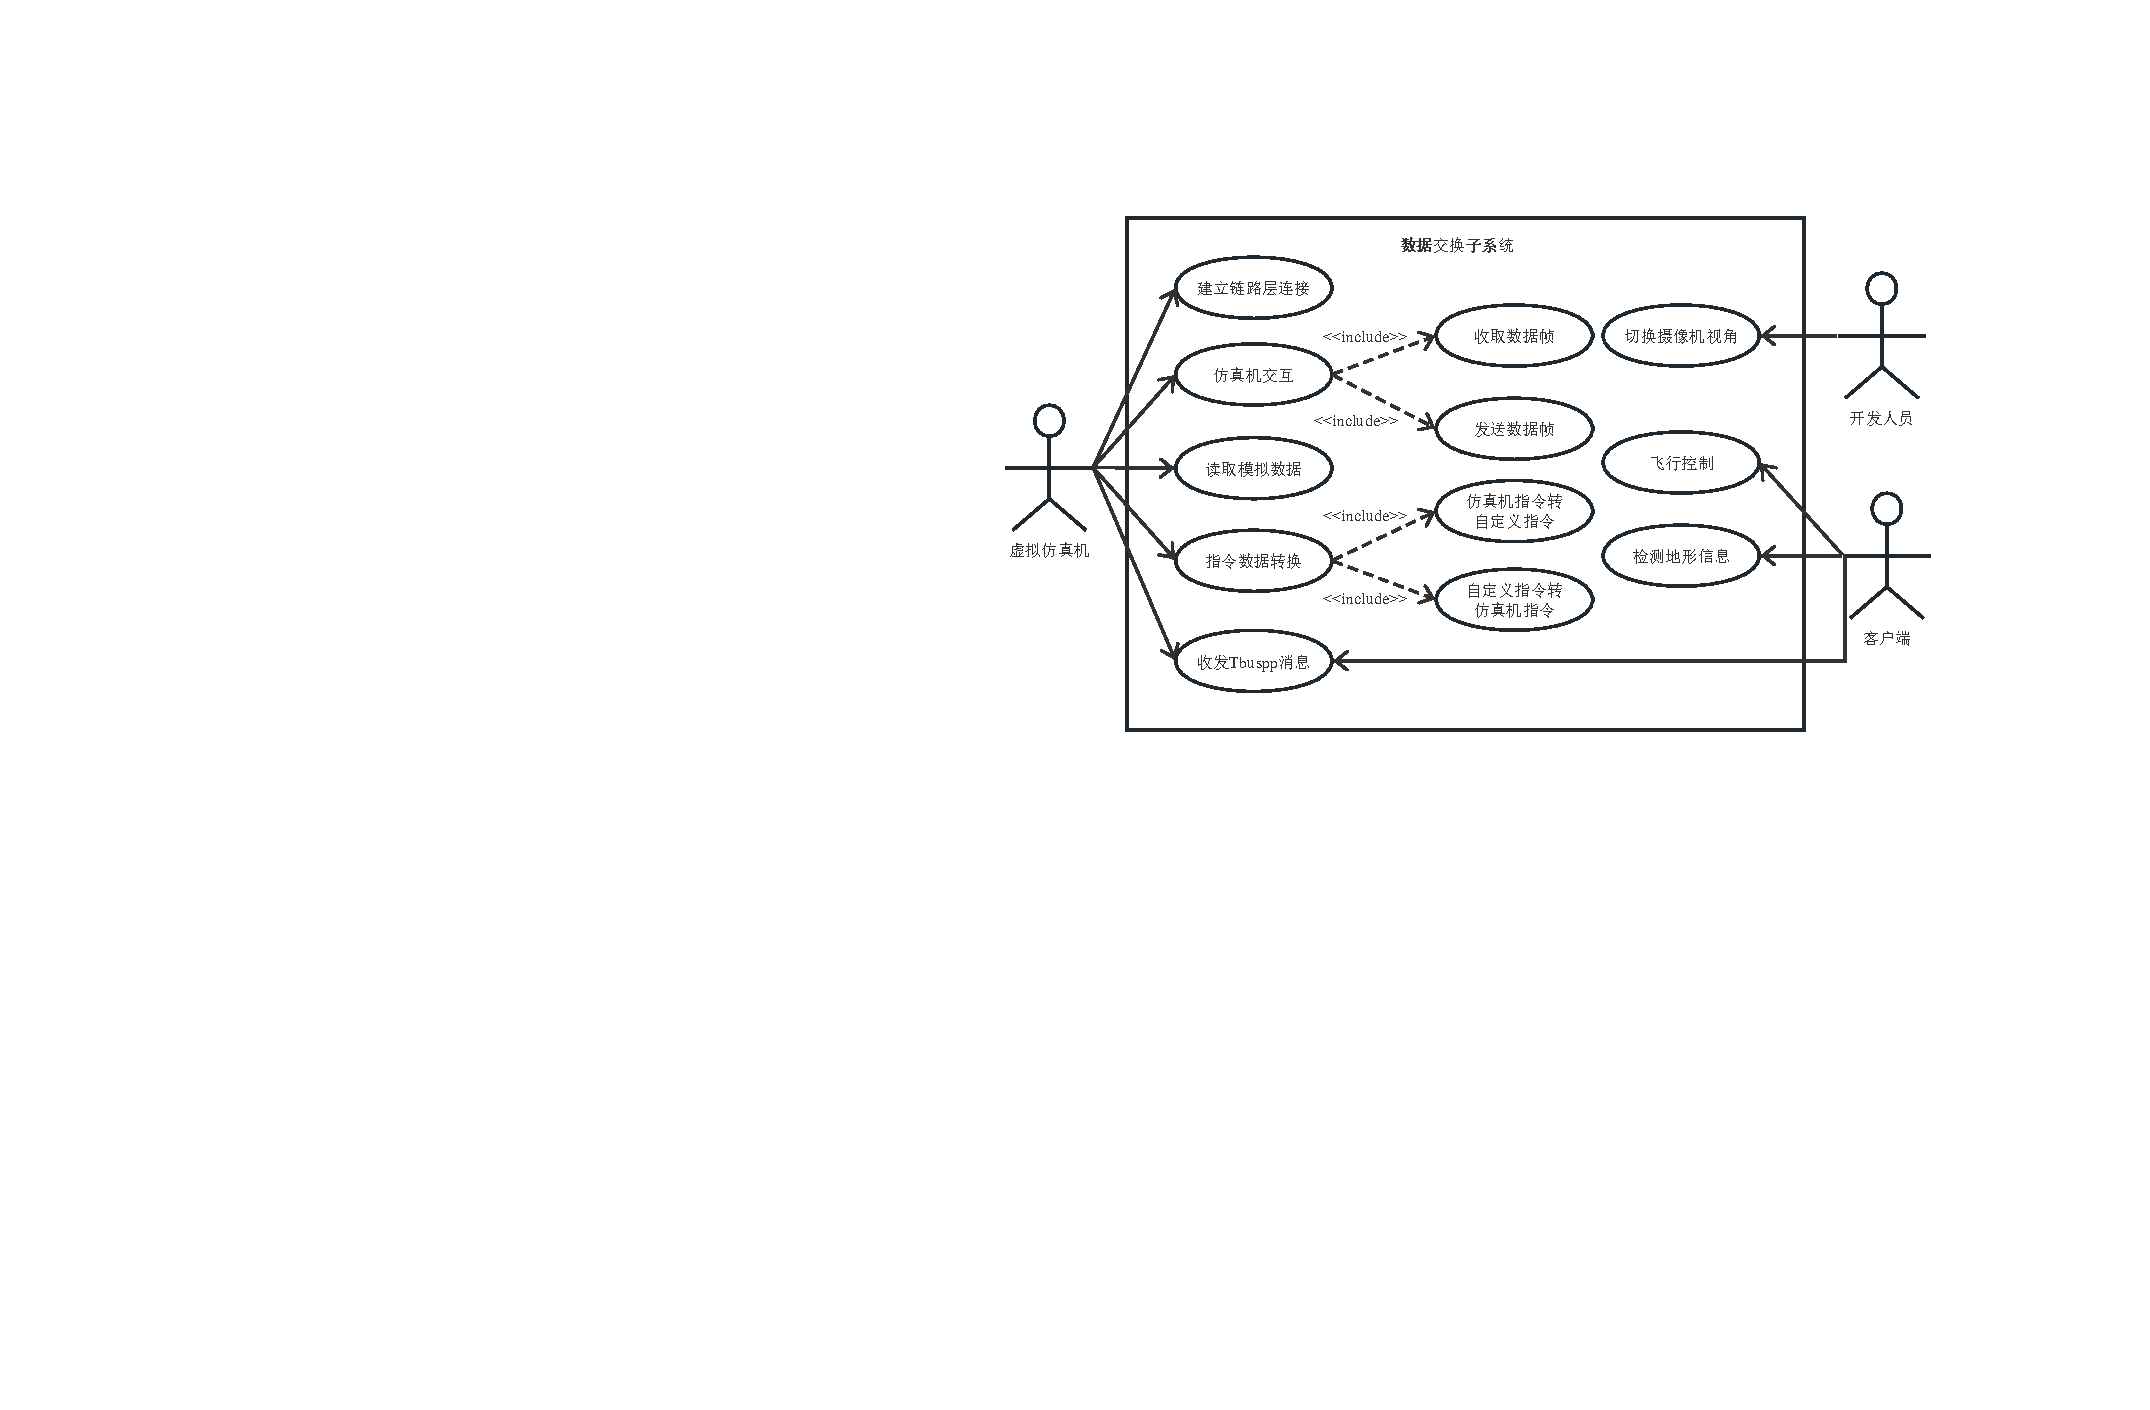
\includegraphics[width=\textwidth]{pictures/usecase.pdf}
        \caption{数据交换子系统用例图}
        \label{usecase}
    \end{center}
\end{figure}

\par
下面将对用例图中提到的系统用例通过用例描述表的形式进行详细解释。
\par
建立链路层连接,是虚拟仿真机与仿真机建立沟通路径的方式。如图\ref{datastruct}中的CAE仿真机数据帧结构所示,由于仿真机是底层设备,其产生的数据帧不含有IP头、TCP头等信息,
所以不能直接交由虚拟仿真机运行环境中的网络协议栈处理,必须由虚拟仿真机亲自侦听网卡上的原始数据帧,并亲自解封或封装。用例的具体情况如表\ref{usecase1}所示。
\begin{figure}[h!]
    \begin{center}
        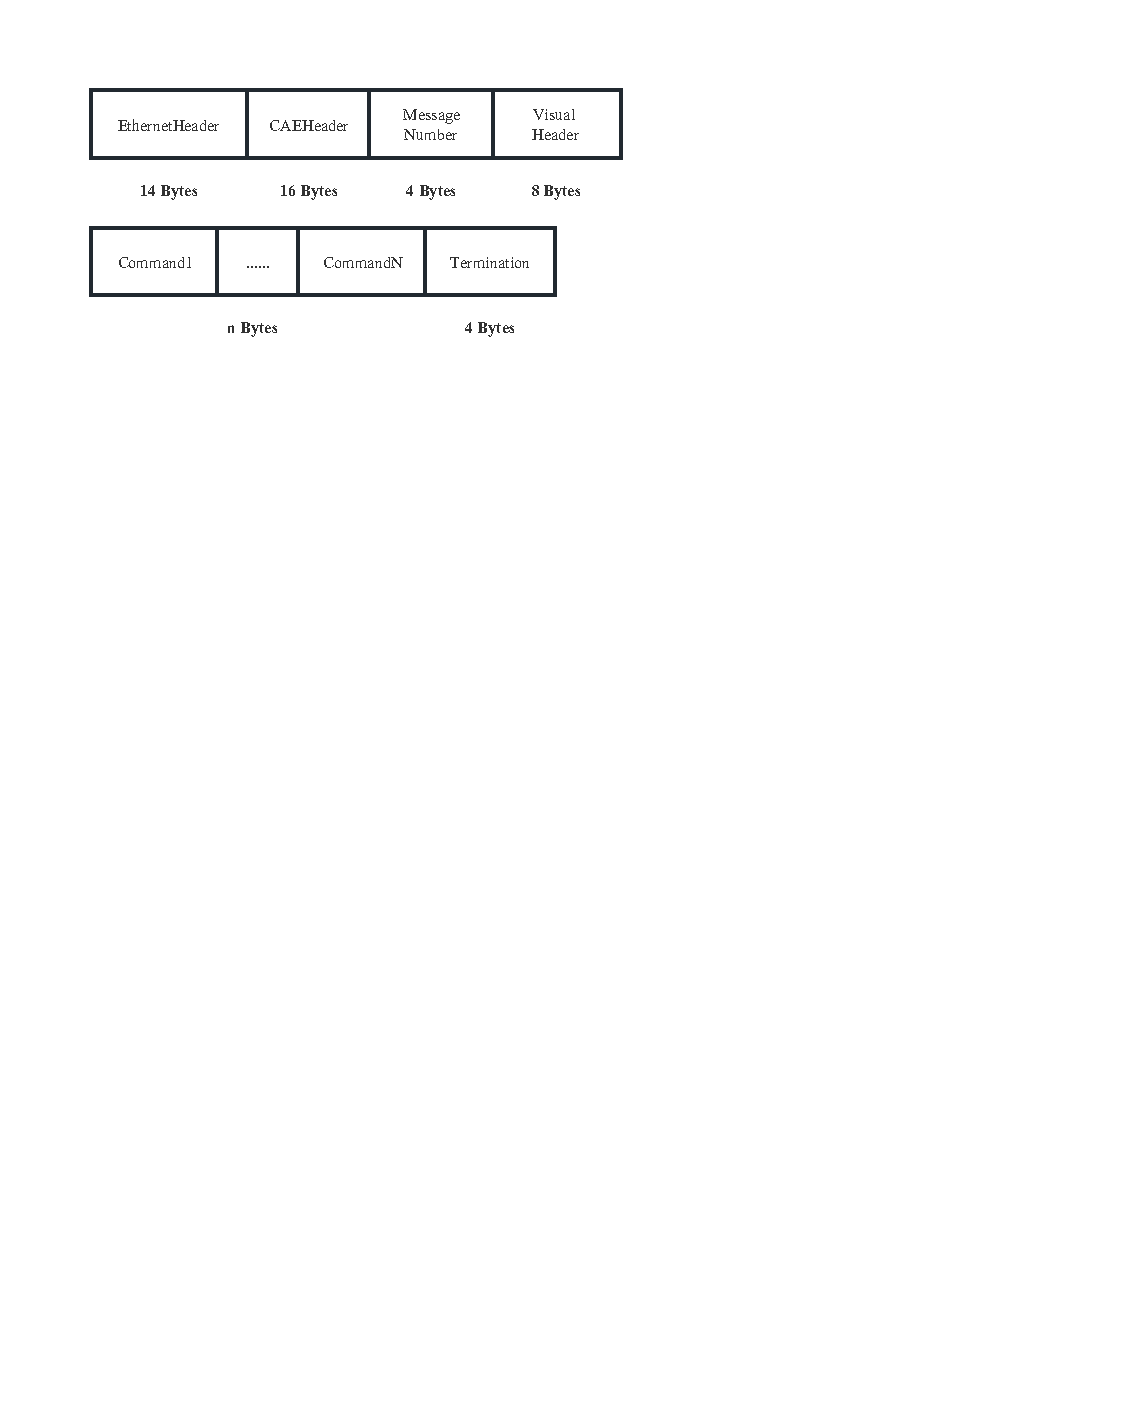
\includegraphics[width=.8\textwidth]{pictures/datastruct.pdf}
        \caption{CAE仿真机数据帧结构}
        \label{datastruct}
    \end{center}
\end{figure}
\begin{table}[htbp]
    \begin{center}
        \caption{建立链路层连接用例描述表}
        \label{usecase1}
        \renewcommand\arraystretch{1.5}
        \begin{tabularx}{0.8\textwidth}{ 
            | >{\centering\arraybackslash\hsize=.5\hsize\linewidth=\hsize}X 
            | >{\raggedright\arraybackslash\hsize=1.5\hsize\linewidth=\hsize}X 
            | }
            \hline
            \textbf{ID} & \textbf{UC1}\\
            \hline
            参与者 & 虚拟仿真机\\
            \hline
            触发条件 & 视景系统开始运行。\\
            \hline
            前置条件 & 1.虚拟仿真机处于接收仿真机消息模式。\par2.仿真机处于开启状态。\\
            \hline
            后置条件 & 能够与仿真机进行数据交流。\\
            \hline
            优先级 & 高\\
            \hline
            正常流程 &  1.查找运行环境下的网络适配器列表。\par 2.选择其中一个网络适配器。\par 3.获取混杂模式数据包捕获句柄。\par 4. 开启及时转发模式。\\
            \hline
            扩展流程 & 网络适配器不能正常运作,打印错误提示。\\
            \hline
        \end{tabularx}
    \end{center}
\end{table}
\par
收取数据帧,是虚拟仿真机从网卡上读取仿真机发送的数据帧的过程。此过程不依靠网络协议栈自动解封,而是自己实现解封过程。收取具体情况如表\ref{usecase2}所示。
\begin{table}[htbp]
    \begin{center}
        \caption{收取数据帧用例描述表}
        \label{usecase2}
        \renewcommand\arraystretch{1.5}
        \begin{tabularx}{0.8\textwidth}{ 
            | >{\centering\arraybackslash\hsize=.5\hsize\linewidth=\hsize}X 
            | >{\raggedright\arraybackslash\hsize=1.5\hsize\linewidth=\hsize}X 
            | }
            \hline
            \textbf{ID} & \textbf{UC2}\\
            \hline
            参与者 & 虚拟仿真机\\
            \hline
            触发条件 & 仿真机向视景系统发送数据帧。\\
            \hline
            前置条件 & 虚拟仿真机侦听了正确的网卡。\\
            \hline
            后置条件 & 数据帧被分为一个个指令段。\\
            \hline
            优先级 & 高\\
            \hline
            正常流程 & 1.去除数据帧头部信息。\par 2.读取指令长度并按该长度截取。\par 3.将数据段加入指令集合。\par 4.回到流程2循环至全部数据读取结束。\\
            \hline
            扩展流程 & 无\\
            \hline
        \end{tabularx}
    \end{center}
\end{table}
\par
发送数据帧,是虚拟仿真机发送信息到仿真机的过程,此过程同样不依靠网络协议栈自动封装,而是自己实现封装过程。具体情况如表\ref{usecase3}所示。
\begin{table}[htbp]
    \begin{center}
        \caption{发送数据帧用例描述表}
        \label{usecase3}
        \renewcommand\arraystretch{1.5}
        \begin{tabularx}{0.8\textwidth}{ 
            | >{\centering\arraybackslash\hsize=.5\hsize\linewidth=\hsize}X 
            | >{\raggedright\arraybackslash\hsize=1.5\hsize\linewidth=\hsize}X 
            | }
            \hline
            \textbf{ID} & \textbf{UC3}\\
            \hline
            参与者 & 虚拟仿真机\\
            \hline
            触发条件 & 反馈指令到达。\\
            \hline
            前置条件 & 虚拟仿真机侦听了正确的网卡。\\
            \hline
            后置条件 & 仿真机收到视景系统反馈并通知其它系统协同。\\
            \hline
            优先级 & 高\\
            \hline
            正常流程 & 1.反馈指令数据段到达。\par 2.将多条指令按规则粘合在一个数据包中。\par 3.为数据包添加以太网头尾信息。\par 4.将数据帧加入发送队列中。\\
            \hline
            扩展流程 & 无。\\
            \hline
        \end{tabularx}
    \end{center}
\end{table}
\par
国内的FFS全部位于航空公司的训练基地内,其价格昂贵且巨大,无法搬运至开发环境中。在日常开发中,虚拟模拟机需要读取文件中的模拟数据来驱动视景系统运作。具体情况如表\ref{usecase4}所示。
\begin{table}[htbp]
    \begin{center}
        \caption{读取模拟数据用例描述表}
        \label{usecase4}
        \renewcommand\arraystretch{1.5}
        \begin{tabularx}{0.8\textwidth}{ 
            | >{\centering\arraybackslash\hsize=.5\hsize\linewidth=\hsize}X 
            | >{\raggedright\arraybackslash\hsize=1.5\hsize\linewidth=\hsize}X 
            | }
            \hline
            \textbf{ID} & \textbf{UC4}\\
            \hline
            参与者 & 虚拟仿真机\\
            \hline
            触发条件 & 使用模拟数据驱动视景系统运作。\\
            \hline
            前置条件 & 虚拟仿真机处于读取模拟数据模式。\\
            \hline
            后置条件 & 文本信息被转化为数据帧信息。\\
            \hline
            优先级 & 高\\
            \hline
            正常流程 & 1.指定文件路径。\par 2.按行读取文本。\par 3.将16进制字符两两一组转换为一个字节。\par 4.按用例二中的流程进行。\\
            \hline
            扩展流程 & 文件不存在或格式有错误则产生警告。\\
            \hline
        \end{tabularx}
    \end{center}
\end{table}

\par
仿真机指令转自定义指令,是虚拟仿真机将难以理解的仿真机指令转换为可供视景系统使用的子定义指令的过程。具体情况如表\ref{usecase5}所示。
\begin{table}[htbp]
    \begin{center}
        \caption{仿真机指令转自定义指令用例描述表}
        \label{usecase5}
        \renewcommand\arraystretch{1.5}
        \begin{tabularx}{0.8\textwidth}{ 
            | >{\centering\arraybackslash\hsize=.5\hsize\linewidth=\hsize}X 
            | >{\raggedright\arraybackslash\hsize=1.5\hsize\linewidth=\hsize}X 
            | }
            \hline
            \textbf{ID} & \textbf{UC5}\\
            \hline
            参与者 & 虚拟仿真机\\
            \hline
            触发条件 & 存在待转换的仿真机指令。\\
            \hline
            前置条件 & 定义了对应仿真机指令的自定义指令。\\
            \hline
            后置条件 & 构建了一个自定义指令。\\
            \hline
            优先级 & 高\\
            \hline
            正常流程 & 1.获取仿真机指令中的指令代号。\par 2.根据指令代号查找对应的转换器。\par 3.使用转换器完成转换。\\
            \hline
            扩展流程 & 对于暂时使用不到的仿真机指令直接丢弃。\\
            \hline
        \end{tabularx}
    \end{center}
\end{table}

\par
自定义指令转仿真机指令,是反馈信息时虚拟仿真机将自定义指令翻译为仿真机使用的仿真机指令的过程。具体情况如表\ref{usecase6}所示。
\begin{table}[htbp]
    \begin{center}
        \caption{自定义指令转仿真机指令用例描述表}
        \label{usecase6}
        \renewcommand\arraystretch{1.5}
        \begin{tabularx}{0.8\textwidth}{ 
            | >{\centering\arraybackslash\hsize=.5\hsize\linewidth=\hsize}X 
            | >{\raggedright\arraybackslash\hsize=1.5\hsize\linewidth=\hsize}X 
            | }
            \hline
            \textbf{ID} & \textbf{UC6}\\
            \hline
            参与者 & 虚拟仿真机\\
            \hline
            触发条件 &  存在待转换的自定义指令。\\
            \hline
            前置条件 & 无\\
            \hline
            后置条件 & 构建了一个仿真机指令。\\
            \hline
            优先级 & 高\\
            \hline
            正常流程 & 1.获取自定义指令的指令代号。\par 2.根据指令代号查找对应的转换器。\par 3.使用转换器完成转换。\\
            \hline
            扩展流程 & 无\\
            \hline
        \end{tabularx}
    \end{center}
\end{table}
\par
视景系统与虚拟仿真机利用Tbuspp插件进行沟通,双方都需要对Tbuspp消息进行收发。具体情况如表\ref{usecase7}所示。
\begin{table}[htbp]
    \begin{center}
        \caption{收发Tbuspp消息用例描述表}
        \label{usecase7}
        \renewcommand\arraystretch{1.5}
        \begin{tabularx}{0.8\textwidth}{ 
            | >{\centering\arraybackslash\hsize=.5\hsize\linewidth=\hsize}X 
            | >{\raggedright\arraybackslash\hsize=1.5\hsize\linewidth=\hsize}X 
            | }
            \hline
            \textbf{ID} & \textbf{UC7}\\
            \hline
            参与者 & 虚拟仿真机\&客户端\\
            \hline
            触发条件 & 有自定义指令待发送。\\
            \hline
            前置条件 & 双方使用Tbuspp成功建立连接。\\
            \hline
            后置条件 & 无\\
            \hline
            优先级 & 高\\
            \hline
            正常流程 &  数据发送过程:\par 1.用ProtoBuffer协议序列化自定义指令结构。\par 2.将消息写入Tbuspp发送队列。\par 
                       数据接收过程:\par 1.从Tbuspp接收队列读取数据。\par 2.使用ProtoBuffer协议反序列化消息得到自定义指令结构。\\
            \hline
            扩展流程 & 无\\
            \hline
        \end{tabularx}
    \end{center}
\end{table}

\par
视景系统中的飞机需要按照收到的飞行状态在地心地固坐标系下的场景进行运动,主要使用飞机的位置和旋转信息,根据飞行画面可以证明数据交换系统的功能是否正常。具体情况如表\ref{usecase7}所示。
\begin{table}[htbp]
    \begin{center}
        \caption{飞行控制用例描述表}
        \label{usecase8}
        \renewcommand\arraystretch{1.5}
        \begin{tabularx}{0.8\textwidth}{ 
            | >{\centering\arraybackslash\hsize=.5\hsize\linewidth=\hsize}X 
            | >{\raggedright\arraybackslash\hsize=1.5\hsize\linewidth=\hsize}X 
            | }
            \hline
            \textbf{ID} & \textbf{UC8}\\
            \hline
            参与者 & 客户端\\
            \hline
            触发条件 & 客户端收到飞机飞行相关指令数据。\\
            \hline
            前置条件 & 存在飞机实体及对应位置场景资源。\\
            \hline
            后置条件 & 连续更新飞机位置和姿态获得动态视景效果。\\
            \hline
            优先级 & 高\\
            \hline
            正常流程 & 1.获取经纬度海拔和欧拉角信息。\par 2.将LLA坐标转换为ECEF坐标。\par 3.将飞机模型置于场景中该坐标位置。\par 4.根据欧拉角调整飞机姿态。\\
            \hline
            扩展流程 & 无\\
            \hline
        \end{tabularx}
    \end{center}
\end{table}
\par
飞机在运动过程中会实时监测三个起落架竖直下方的地形信息,并将他们作为反馈信息最终给到仿真机,用于进近时与地面碰撞情况的判断。具体情况如表\ref{usecase8}所示。
\begin{table}[htbp]
    \begin{center}
        \caption{检测地形信息用例描述表}
        \label{usecase9}
        \renewcommand\arraystretch{1.5}
        \begin{tabularx}{0.8\textwidth}{ 
            | >{\centering\arraybackslash\hsize=.5\hsize\linewidth=\hsize}X 
            | >{\raggedright\arraybackslash\hsize=1.5\hsize\linewidth=\hsize}X 
            | }
            \hline
            \textbf{ID} & \textbf{UC9}\\
            \hline
            参与者 & 客户端\\
            \hline
            触发条件 & 飞机处于飞行状态。\\
            \hline
            前置条件 & 场景数据库中存在飞机所处位置的地形。\\
            \hline
            后置条件 & 无\\
            \hline
            优先级 & 中\\
            \hline
            正常流程 & 1.飞机位置更新。\par 2.发射射线获取飞机竖直下发的地形高度和飞机离地高度。\par 3.将信息组合成自定义指令。\\
            \hline
            扩展流程 & 无\\
            \hline
        \end{tabularx}
    \end{center}
\end{table}

\par
摄像机的视野决定了最终的画面渲染范围,为了开发人员观察飞机运动情况和机场环境,多种视角摄像机必不可少。三种视角切换可操控摄像机可以对飞机以及其所处场景进行全方位的细致观察。具体情况如表\ref{usecase9}所示。
\begin{table}[htbp]
    \begin{center}
        \caption{切换摄像机视角用例描述表}
        \label{usecase10}
        \renewcommand\arraystretch{1.5}
        \begin{tabularx}{0.8\textwidth}{ 
            | >{\centering\arraybackslash\hsize=.5\hsize\linewidth=\hsize}X 
            | >{\raggedright\arraybackslash\hsize=1.5\hsize\linewidth=\hsize}X 
            | }
            \hline
            \textbf{ID} & \textbf{UC10}\\
            \hline
            参与者 & 开发人员\\
            \hline
            触发条件 & 开发人员按键切换摄像机视角\\
            \hline
            前置条件 & 无\\
            \hline
            后置条件 & 相机可以循环切换。\\
            \hline
            优先级 & 中\\
            \hline
            正常流程 & 1.初始为飞机第一视角摄像机。\par 2.按键切换至第三人称环绕视角,将以飞机为中心环绕观察。\par 3.再次切换为自由摄像机,可使用输入设备在场景中漫游观察。\\
            \hline
            扩展流程 & 无\\
            \hline
        \end{tabularx}
    \end{center}
\end{table}
}

\section{数据交换子系统概要设计}
数据交换子系统的架构设计如图\ref{subframe}所示,整个系统分为三个部分,仿真机与虚拟仿真机间通过数据帧进行交互,虚拟仿真机与游戏引擎通过TCP协议交互。
仿真机的作用是对飞行员的操作输入进行仿真计算,得出飞机状态,这部分由FFS厂商设计开发。虚拟仿真机则将不同的仿真机数据协议翻译为统一的供视景系统使用的指令结构体,以此屏蔽仿真机的差异。
游戏引擎的只需按照收到的指令数据渲染飞行画面,并提供简单的反馈信息。
\par 
在数据交换子系统中虚拟仿真机的通信服务完全使用C++语言开发,游戏引擎中核心功能如通用坐标系转换、射线探测等由C++语言开发。模拟飞行视景系统的专属逻辑如飞行控制则使用Lua脚本。
在开发过程中飞行逻辑需要不断调整优化,且日后仍有如灯光、起落架等大量逻辑加入,Lua作为轻量小巧的解释性语言,非常适合作为游戏开发中不断嵌入的脚本语言。
\par
仿真机侧数据交换使用到WinPcap作为与仿真机数据交换的工具,WinPcap不依靠主机的诸如TCP/IP协议去收发数据包,为应用程序提供访问网络底层的能力。
数据链路层的原始数据帧收发都需要通过WinPcap实现。由于不同厂商的数据帧结构不尽相同,因此数据帧解析和生成会对应不同的实现。
\par
协议转换模块主要负责指令结构体与ProtoBuffer协议结构体之间的转换。谷歌公司的ProtoBuffer数据序列化协议有非常高的生成和解析速度,作为实时渲染的数据交换协议十分适合。
\par
引擎侧数据交换模块则主要负责虚拟仿真机与游戏引擎间的通信。通信内容是由ProtoBuffer封装好的指令数据,通过腾讯通信组件Tbuspp实现通讯。
给到游戏引擎的数据发送频率应当与渲染帧率相一致,对该线程的运行做出限制。
\par
飞行控制模块负责实现飞机的基础飞行功能用于检测数据交换的正确性,其中主要涉及到地理坐标系的转换算法。
同时在基础可操控组件模板下编写了实现了三种可操控摄像机负责观察飞机和场景。

\begin{figure}[htbp]
    \begin{center}
        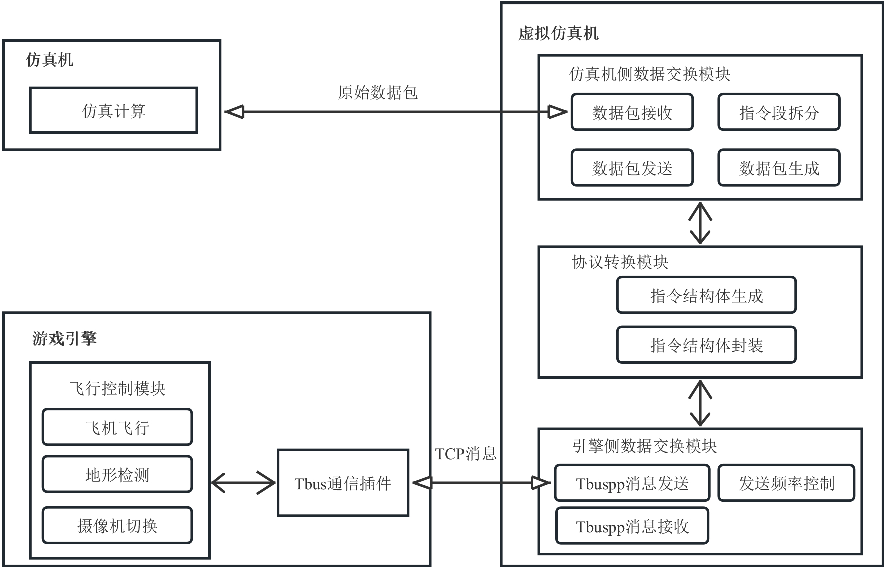
\includegraphics[width=\textwidth]{pictures/framework.pdf}
        \caption{数据交换子系统架构图}
        \label{subframe}
    \end{center}
\end{figure}
\subsection{系统逻辑视图}
逻辑视图以用户为中心,展示了系统的架构和功能模块。系统通过逻辑层次划分,把各个功能抽象成类,实现功能的封装。
如图\ref{logic}描述了系统的逻辑视图。SimNodeCommunicate代表仿真机与虚拟仿真机间沟通的模块,包含EstablishConnection功能,负责建立维持底层网络的连接,在此基础上实现原始数据包的收发;
SendDataFrame和ReceviceDataFrame负责维护各自的消息队列,并真正执行原始数据包的发送和接收任务,前者将数据包交给数据转换模块,后者则将收到的数据反馈给仿真机。
DataConverter表示数据转换模块。来自仿真机的消息会经历原始数据包到中间指令结构体再到ProtoBuffer协议数据段的变换过程,反馈消息则与之相反。
DataAnalysis负责原始数据包重新解释为指令结构体或将结构体添加头部信息封装为原始数据包,DataEncapsulate负责指令结构体与ProtoBuffer结构间的转换。
GameEngineCommunication表示虚拟仿真机与游戏引擎间沟通的模块,使用到了Tbuspp这一插件,EstablishConnection同样负责建立和维持Tbus节点的连接,在此基础上收发TCP数据段。
SendDataSegement和ReceviceDataSegement负责维护各自的消息队列,并真正执行数据段的发送和接收任务,前者将数据段交给游戏逻辑使用,后者将反馈信息给到数据转换模块逆向转换。
GameLogic模块负责飞行模拟的运行逻辑,其中FlightControl模块负责控制飞机位置和旋转姿态,也是最基本的飞行模拟要求。Camera模块负责确定飞行画面渲染的范围,第一人称视角只会跟随飞机运动,环绕视角可以在飞机为中心的球面上移动,自由视角则可以在场景中漫游。
DetectTerrain负责检测飞机低空飞行时其下方的地形信息,此信息会被反馈给仿真机处理。
\begin{figure}[h]
    \begin{center}
        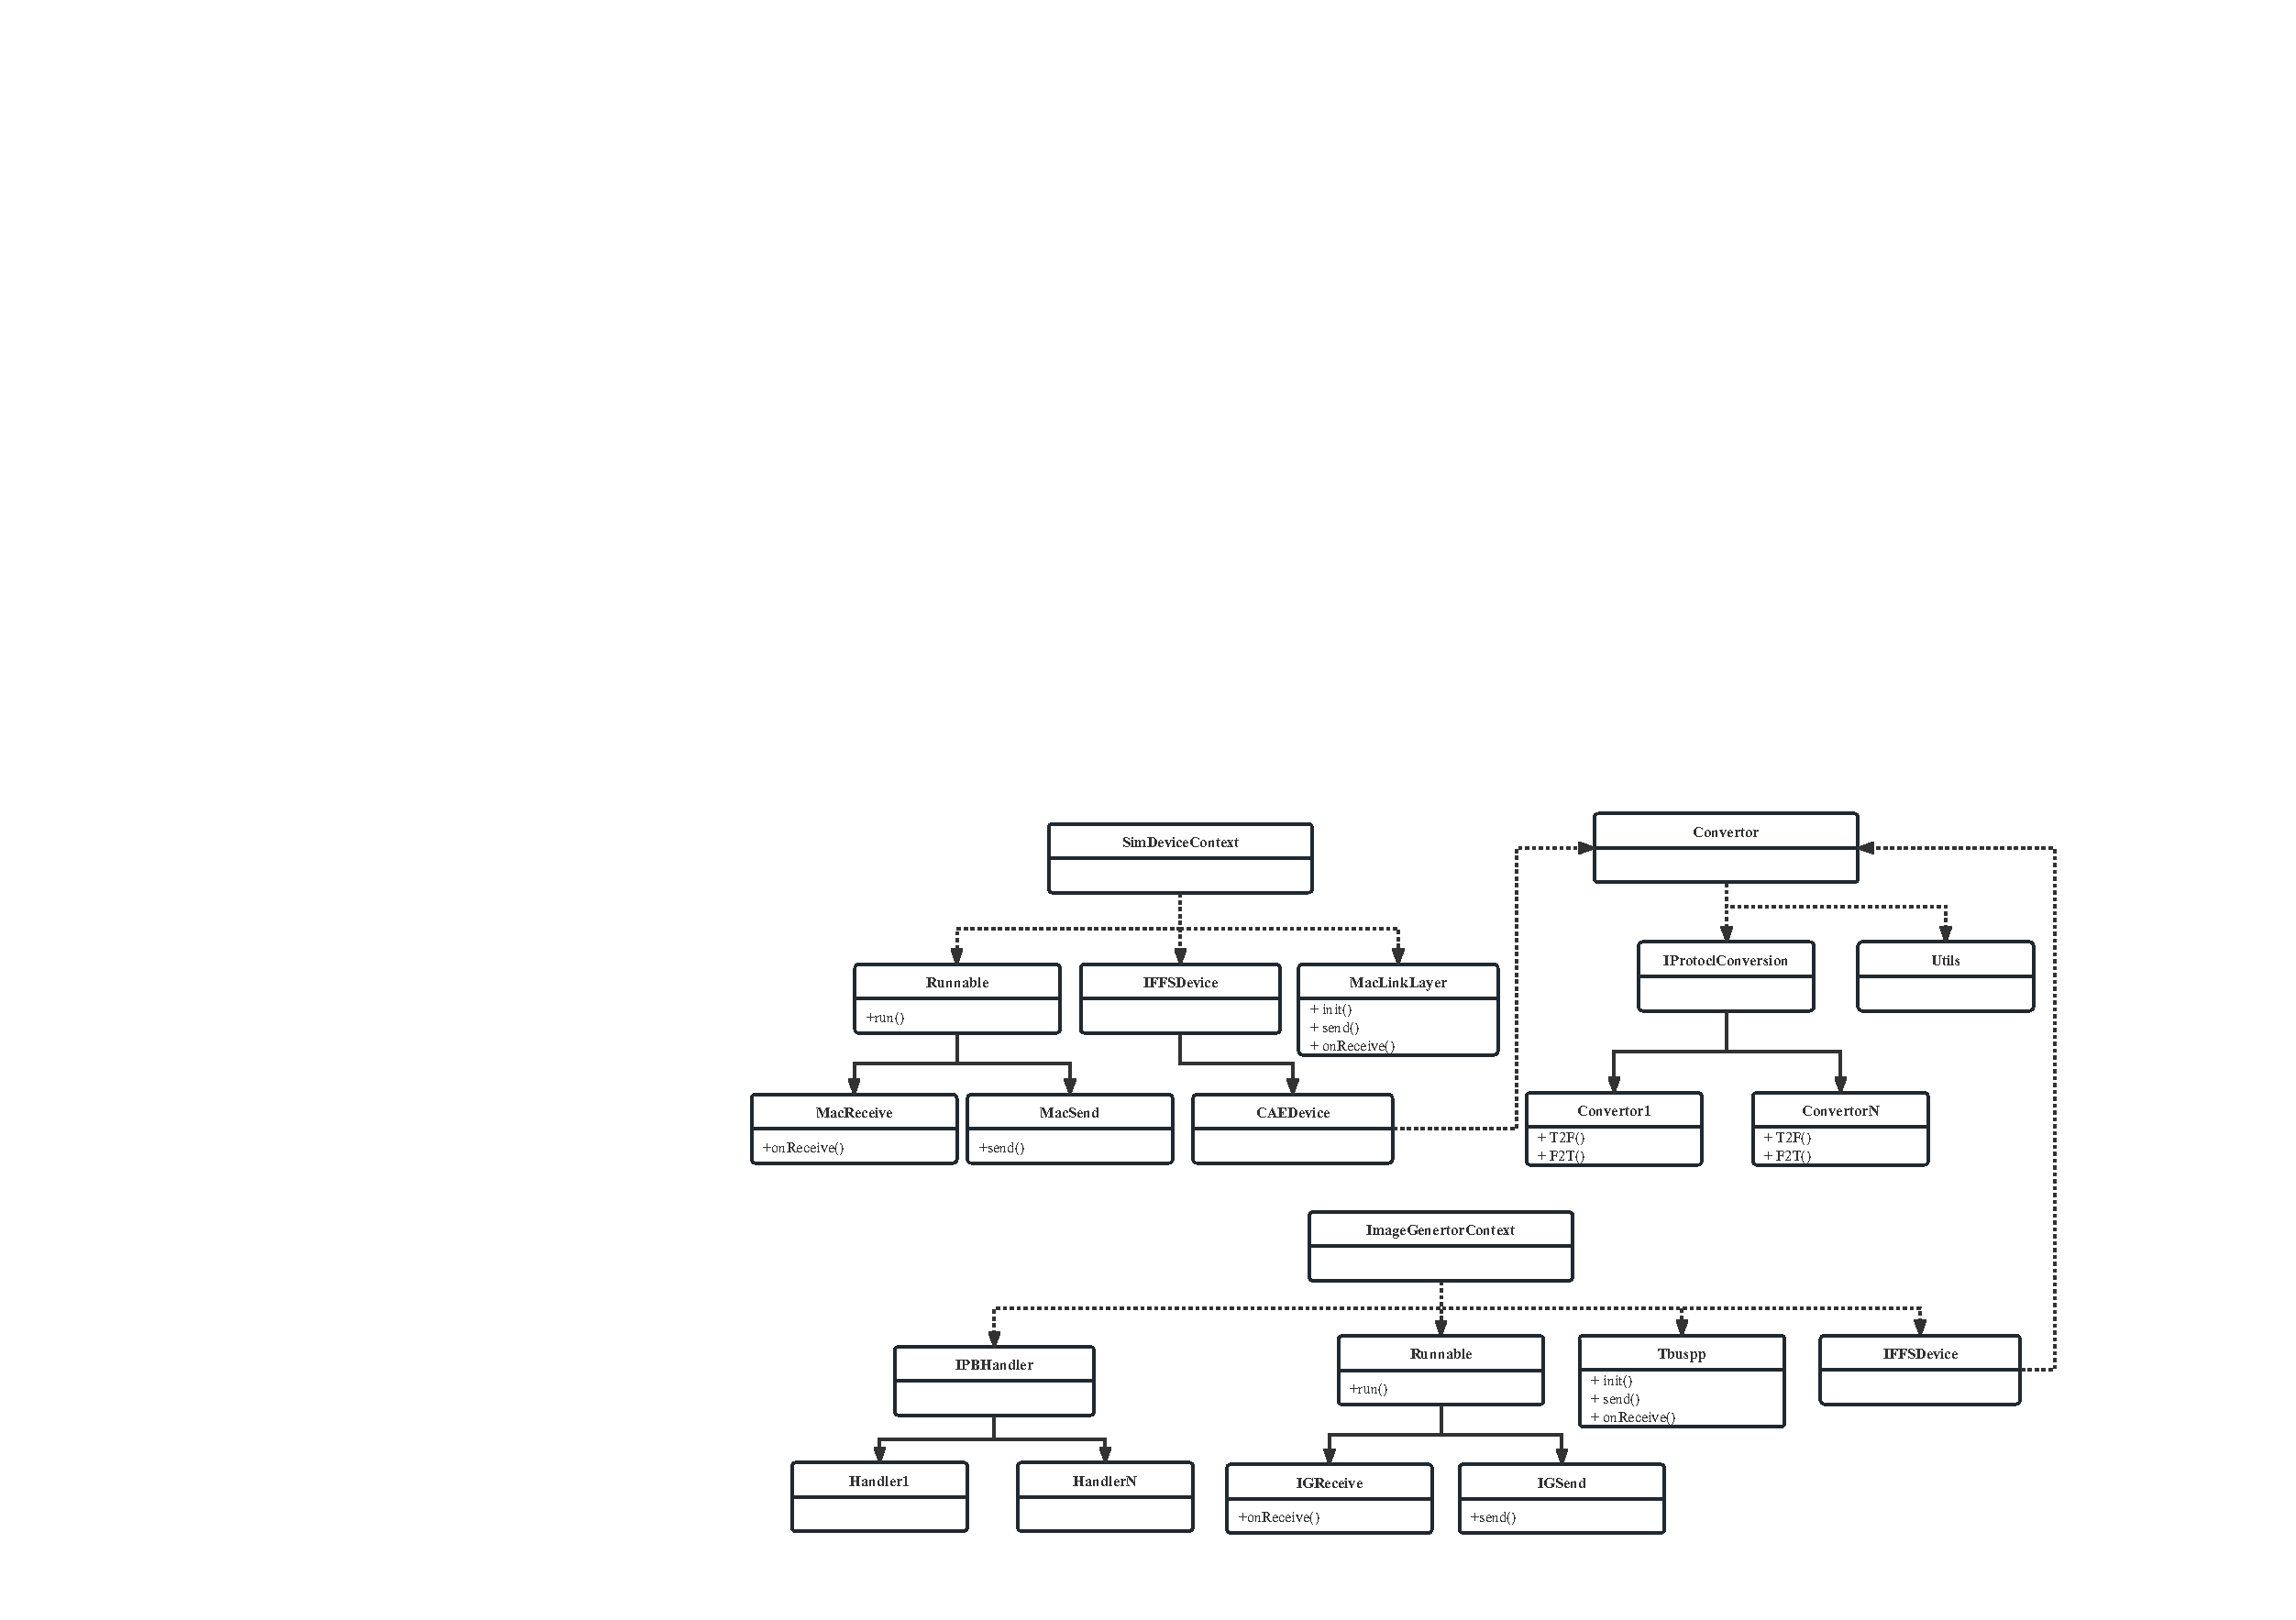
\includegraphics[width=\textwidth]{pictures/logic.pdf}
        \caption{逻辑视图}
        \label{logic}
    \end{center}
\end{figure}
\subsection{系统开发视图}
\begin{figure}[h]
    \begin{center}
        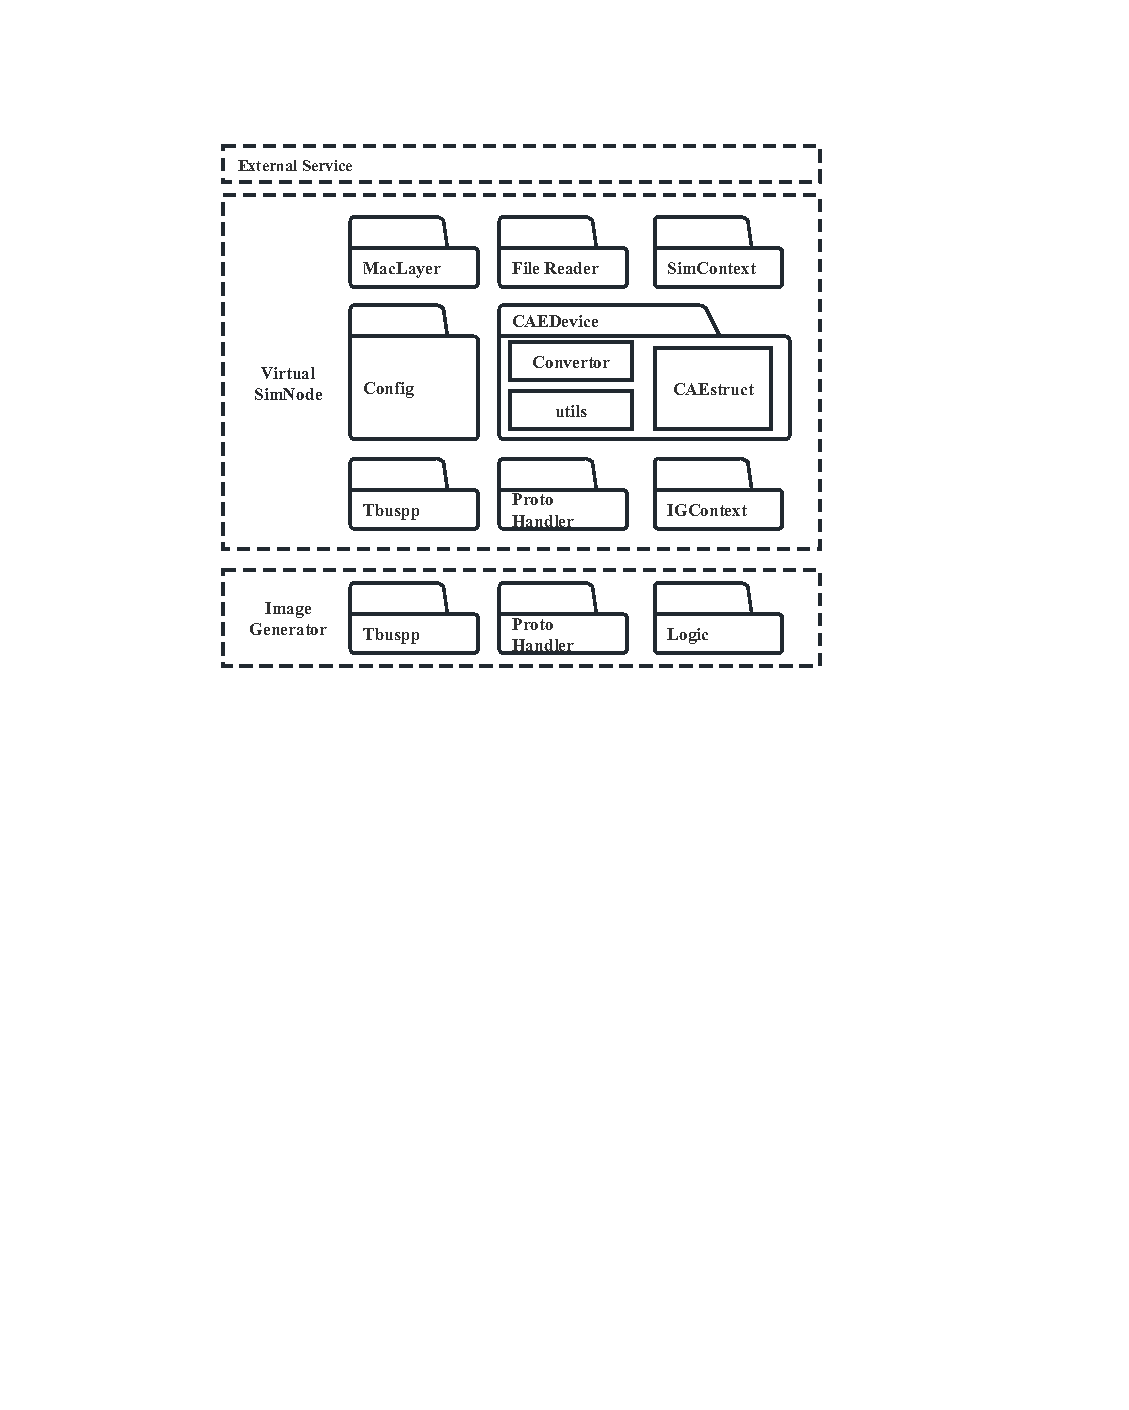
\includegraphics[width=0.8\textwidth]{pictures/devdiagram.pdf}
        \caption{开发视图}
        \label{dev}
    \end{center}
\end{figure}
\subsection{系统进程视图}
进程视图是用系统工程师的视角对系统进行阐述。可以详细阐述系统的动
态运行过程,重点描述系统运行时的行为。图\ref{procedure}是本系统的进程视图,
在虚拟仿真机中,主线程启动后会开启一个发送线程和一个接收线程,负责接收来自仿真机的数据处理后发送给游戏引擎,或者接收来自游戏引擎的反馈给到仿真机。
在游戏引擎中,逻辑线程负责接收到数据后完成对场景的布置,同时与发送线程同步,避免积累太多数据在内存中。逻辑线程同时需要计算碰撞情况并给出反馈信息。
渲染线程专门负责对逻辑线程中生成的场景进行渲染,一般来讲逻辑线程比渲染线程快一帧。

\begin{figure}[h]
    \begin{center}
        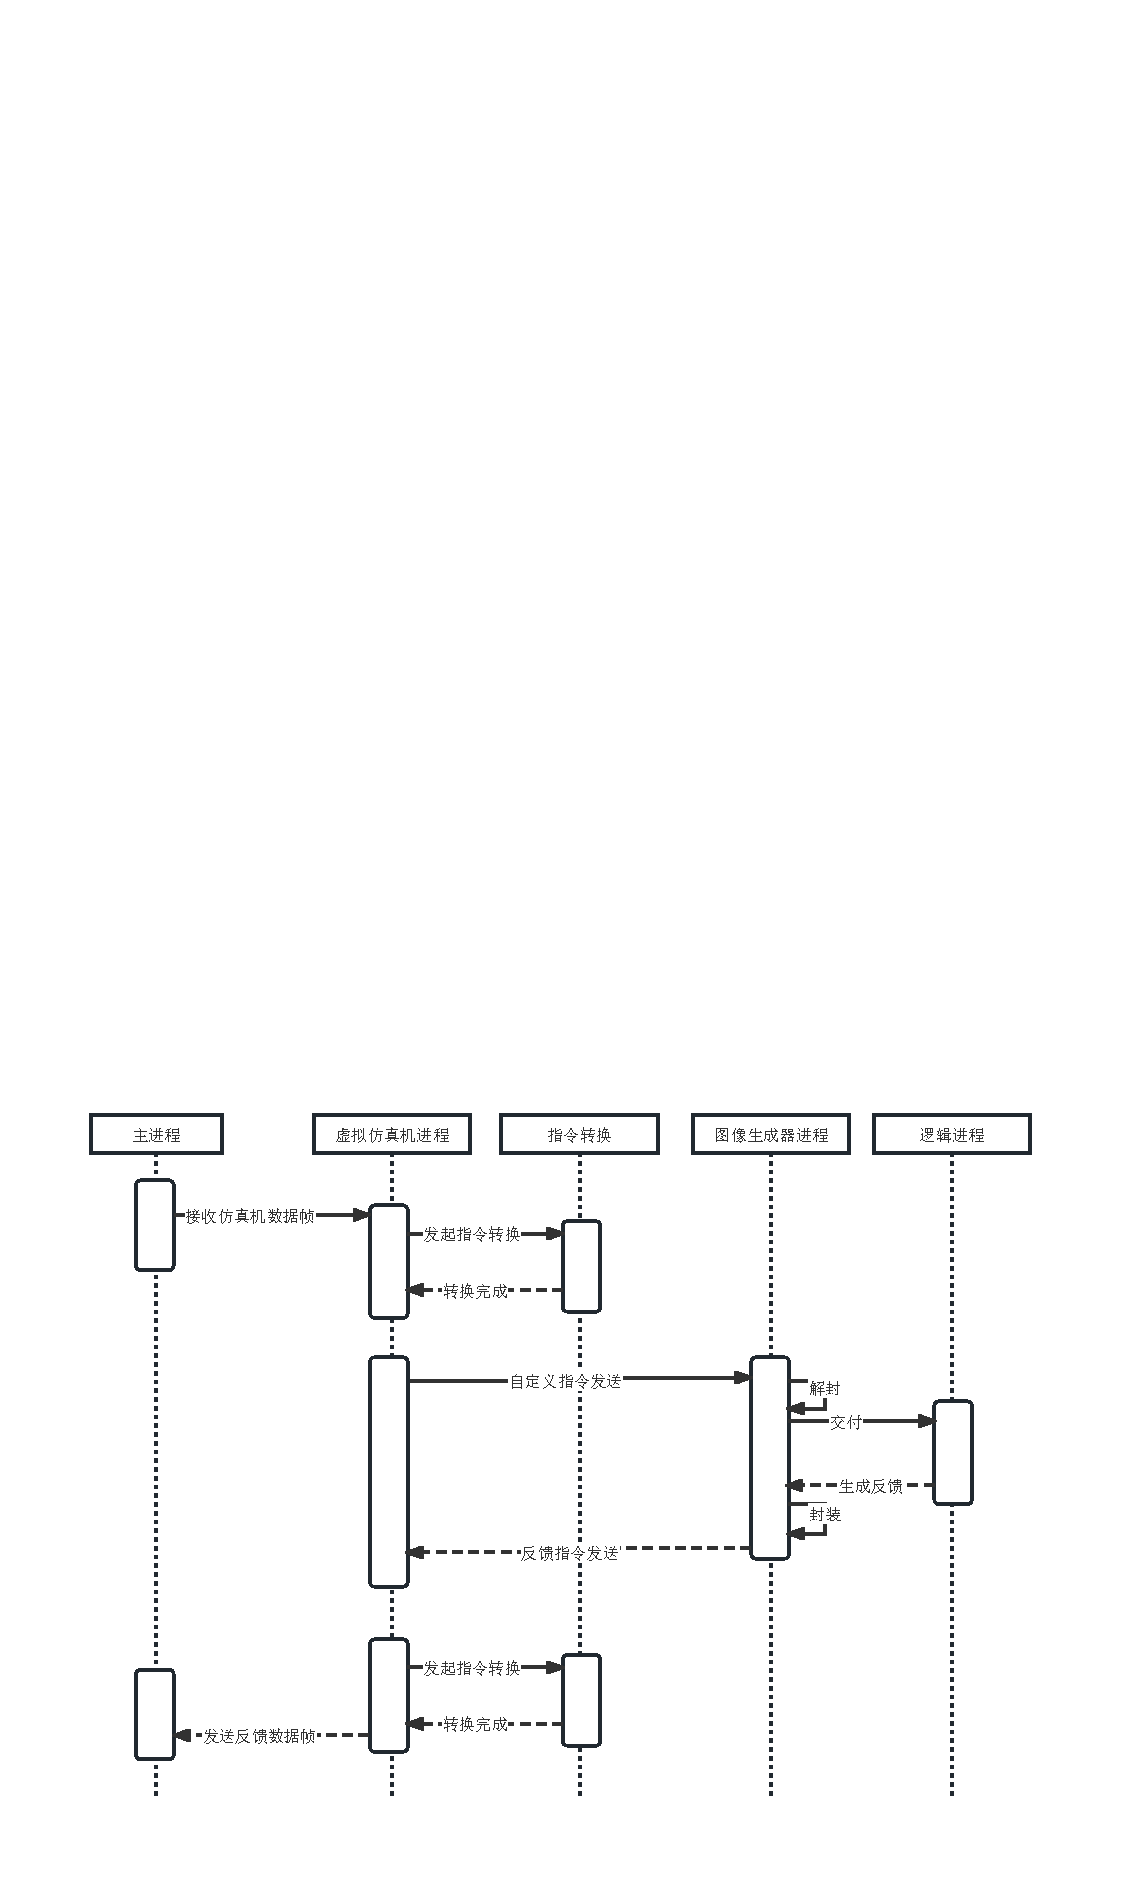
\includegraphics[width=0.8\textwidth]{pictures/procedure.pdf}
        \caption{进程视图}
        \label{procedure}
    \end{center} 
\end{figure}
\subsection{系统部署视图}
部署视图是用运维人员的视角对系统进行阐释。它着重于解释说明系
统的整体物理结构,包括各组件之间的连接方式等等,又称为物理视图。图\ref{deploydiagram}是本系
统的部署视图。飞行员在机舱中操作被仿真机记录并进行仿真计算,数据的解析和转换在虚拟仿真机内完成,游戏引擎收到TCP消息后完成场景的生成和渲染。
\begin{figure}[h]
    \begin{center}
        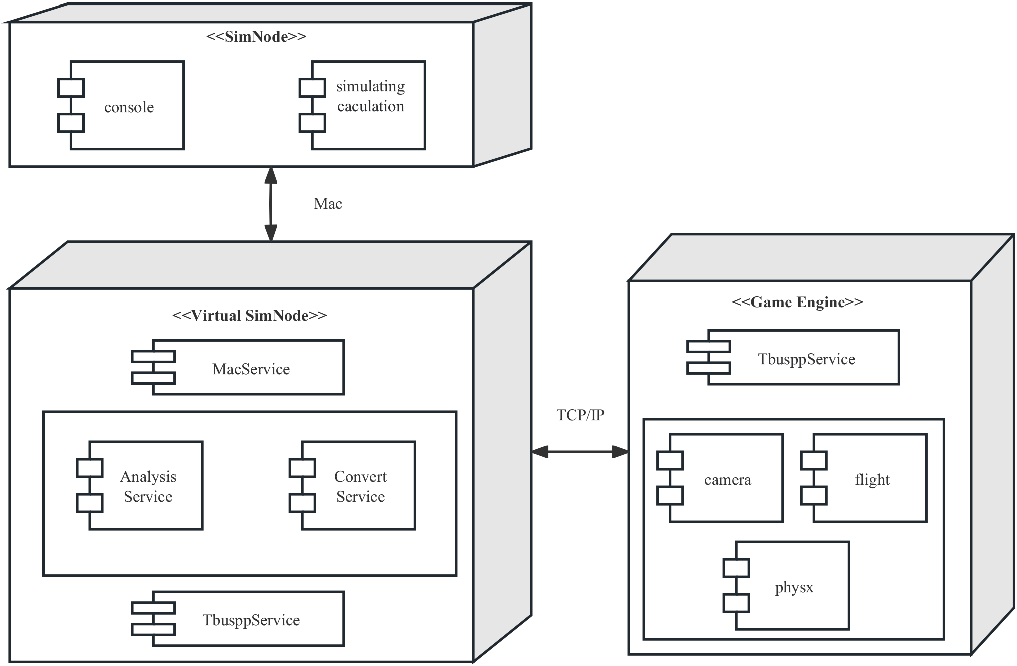
\includegraphics[width=0.8\textwidth]{pictures/deploydiagram.pdf}
        \caption{部署视图}
        \label{deploydiagram}
    \end{center}
\end{figure}
\section{数据交换子系统详细设计}
\subsection{仿真机侧数据交互模块}
仿真机侧数据交换模块负责虚拟仿真机与仿真机之间的交流。他们之间通过数据链路层的原始数据包进行沟通,即除去真实数据外,仅含有Mac地址等信息。因此不能依靠TCP/IP协议收发而是直接访问底层网络。
该模块会将到来的数据帧拆为指令结构体供后续使用,或者将指令结构体包装为数据帧发送给仿真机。
\par
本模块的主要执行流程如图\ref{module11}所示。流程分为接收消息和发送反馈消息两部分。在接收到消息后,需要先读取数据帧中的指令代号信息,如果代号已知,则调取对应的转换对象,将其中信息重新解释为对应的指令结构体。
由于指令代号有接近百种,项目初期只用到部分指令,对于未知的指令进行抛弃。发送反馈消息过程中,则需要对指令结构体添加数据帧头部信息,并通过底层网络直接发送。

\begin{figure}[h!]
    \begin{center}
        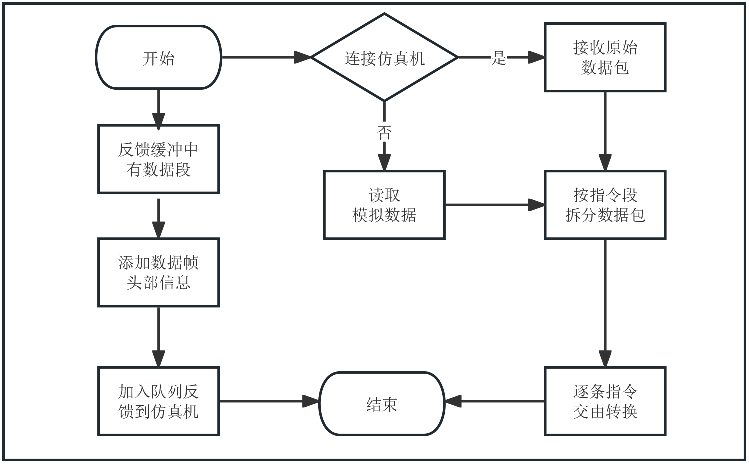
\includegraphics[width=0.8\textwidth]{pictures/flowchart1.pdf}
        \caption{仿真机侧数据交互流程图}
        \label{module11}
    \end{center}
\end{figure}
\par
本模块的核心类图如图\ref{module12}所示。其中的核心是类SimulationDeviceContext,它表示在虚拟仿真机中与仿真机交流的环境,其中包含控制信息收发的线程和待发送信息队列。
ISimulatorDeviceInterface则是与仿真机交流的接口,其中包含了对于数据帧中指令代号的读取方法GetSimOperateCode,以及发送消息给仿真机SendToSimulationDevice方法。
FullFightSimulatorDeviceBase中包含对该接口的实现。CAEGenericSimulatorDeviceBase代表CAE公司FFS设备,其中含有解读并转换该设备原始数据包的具体算法。当需要接入其他公司设备时,
只需要重新设计对应方法即可。
MacLinkCommunication类负责建立数据链路层连接并与真实仿真机进行原始数据包的交流。
\begin{figure}[h!]
    \begin{center}
        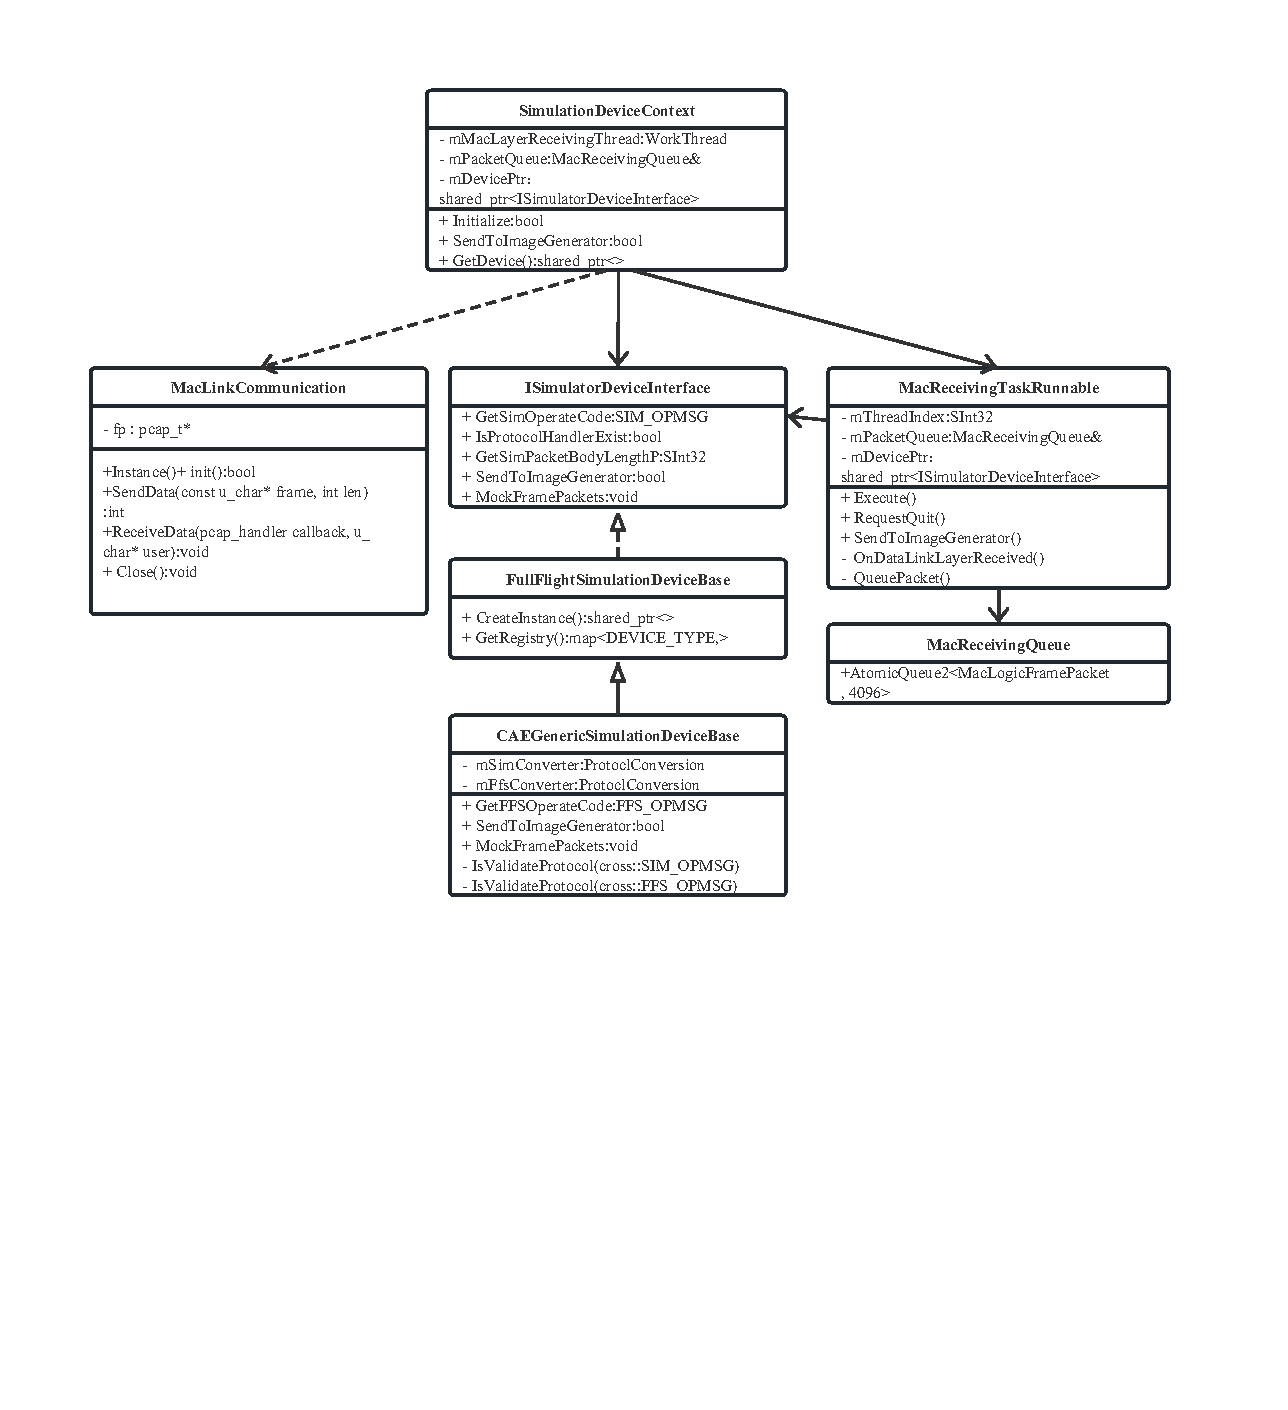
\includegraphics[width=\textwidth]{pictures/classdiagram1.pdf}
        \caption{仿真机侧数据交互核心类图}
        \label{module12}
    \end{center}
\end{figure}

\subsection{数据转换模块}
协议转换模块负责指令结构体与ProtoBuffer协议结构间的封装与解封。从仿真机收到的消息中对于浮点数的表达方式是由该厂商自行设计的,对于不同精度要求的数据表示方式也存在差异。
因此这两种结构之间的转换需要严格依照设计文档中的说明设计转换算法,而不是简单的赋值。ProtoBuffer协议结构为给到游戏引擎的数据结构,指令结构体则是准备反馈给仿真机的结构。
\par
本模块的主要执行流程如图\ref{module21}所示。在封装的过程中,需要先确定该指令对应的ProtoBuffer结构,经过数据转换算法后得到该结构,之后添加部分头部信息便可将其加入发送队列。
解封时现根据头部信息确定指令类型,再使用逆向的数据转换算法生成指令结构体即可准备发送给仿真机。

\begin{figure}[h!]
    \begin{center}
        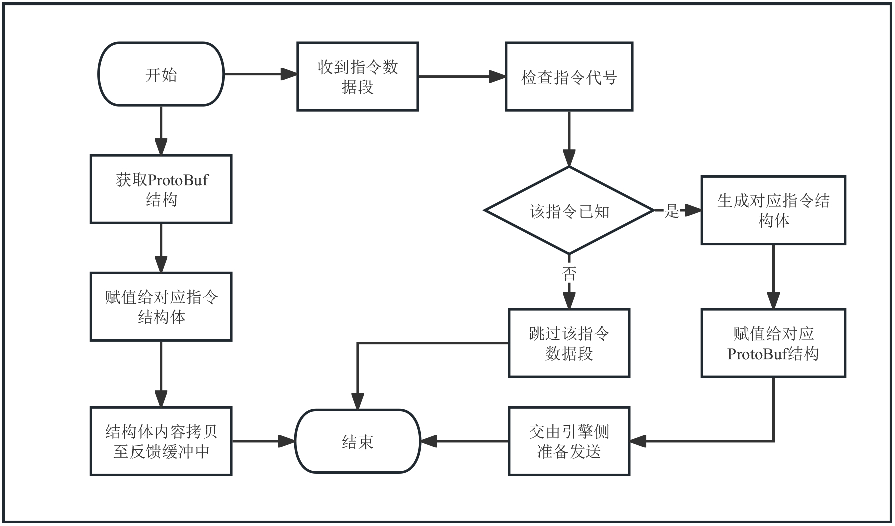
\includegraphics[width=0.8\textwidth]{pictures/flowchart2.pdf}
        \caption{数据转换流程图}
        \label{module21}
    \end{center}
\end{figure}
\par
本模块的核心类图如图\ref{module22}所示。其中核心为IProtoclConversion接口,其中声明了指令结构体与ProtoBuffer协议结构体互相转换的两种方法Convert。
ProtoclConversion是一个模板类,成员属性T表示一个指令结构体,成员属性F表示一个ProtoBuffer协议结构体,T和F组成互相转换的一对。该模板实例化的对象调用Convert方法便可以调用到对应结构体的转换方法。
SD\_PACKET\_21H是一个指令结构体的实例类型,包含了经纬度欧拉角等飞机飞行信息,其中也含有该指令类型转换的具体方法,发送给仿真机的队列MacLogicFramePacket由添加了数据帧头的指令结构体构成。
GeodeticCSUpdateStruct为SD\_PACKET\_21H指令结构体对应的ProtoBuffer协议结构体,发送给游戏引擎的消息队列FfsLogicFramePacket由各种ProtoBuffer协议结构体组成。

\begin{figure}[h!]
    \begin{center}
        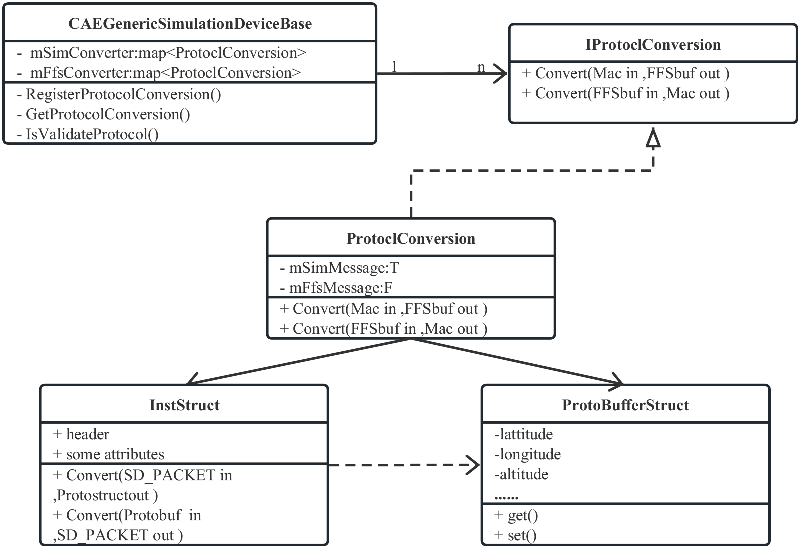
\includegraphics[width=\textwidth]{pictures/classdiagram2.pdf}
        \caption{数据转换核心类图}
        \label{module22}
    \end{center}
\end{figure}
\subsection{图像生成器侧数据交互模块}
游戏引擎侧数据交换模块负责虚拟仿真机与游戏引擎之间的交流。其利用Tbuspp插件使用TCP消息沟通,数据交换协议则是ProtoBuffer。再发送给游戏引擎的过程中,需要将发送频率的固定,因此该线程会以固定的频率被唤醒。
\par
本模块的主要执行流程如图\ref{module31}所示。当发送队列中有消息时,若可以进行发送则直接发送,否则要等待新的发送时机。反馈消息接收时则不需考虑频率,直接接收消息并给到协议转换模块。
\begin{figure}[h!]
    \begin{center}
        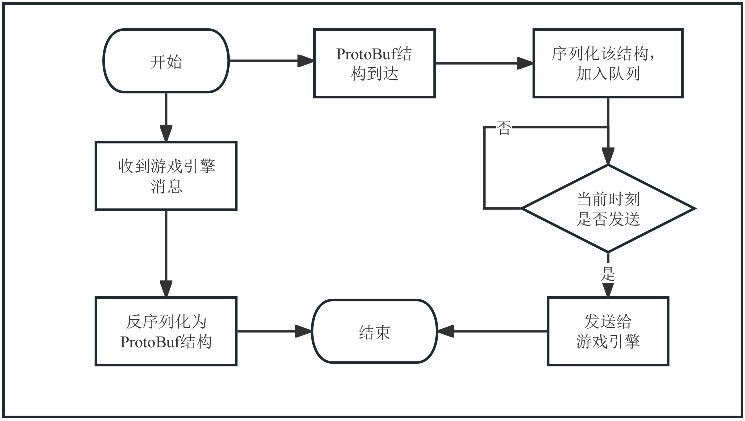
\includegraphics[width=0.8\textwidth]{pictures/flowchart3.pdf}
        \caption{视景系统侧数据交互流程图}
        \label{module31}
    \end{center}
\end{figure}
\par
本模块的核心类图如图\ref{module32}所示。其中的核心是类ImageGeneratorContext,它表示在虚拟仿真机中与游戏引擎交流的环境,其中包含控制信息收发的线程和信息队列。
IImageGeneratorDeviceInterface则是与游戏引擎交流的接口,其中包含了对于ProtoBuffer结构中指令代号的读取方法GetOperateCode,以及发送消息给游戏引擎SendToImageGenerator方法。
FullFightSimulatorDeviceBase是对该接口的实现,其依赖控制发送频率的类FrameSynchronization。CAEGenericSimulatorDeviceBase代表CAE公司FFS设备,其中含有与该公司设备进行沟通的具体方法。
\begin{figure}[h!]
    \begin{center}
        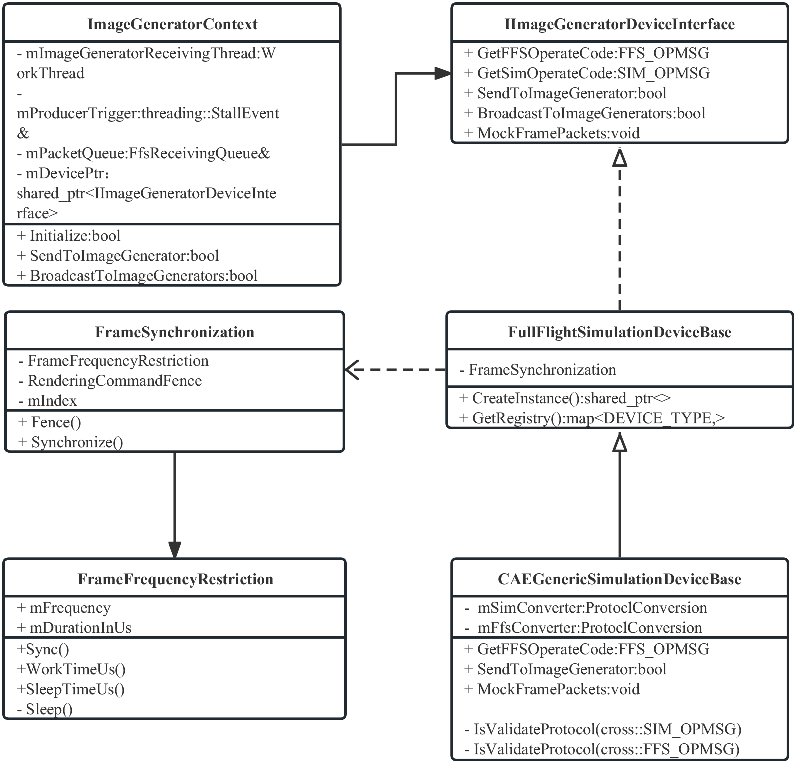
\includegraphics[width=\textwidth]{pictures/classdiagram3.pdf}
        \caption{视景系统侧数据交互核心类图}
        \label{module32}
    \end{center}
\end{figure}
\subsection{数据同步模块}
\subsection{飞行数据处理模块}
基础飞行控制模块负责让视景系统中的飞机运动起来并能被开发人员细致观察。实际过程中,游戏引擎会根据接收的数据实时改变飞机位置和飞行姿态,并加载周边场景信息。
飞机会随时对当前竖直下方的地形信息进行探测,并作为反馈信息。飞行过程中开发人员可以进行三种视角的观察。
\par
本模块的主要执行流程如图\ref{module41}所示。对于不用于飞机位置的指令直接跳过。对于位置和姿态信息则需要一定的转换,因为其在指令中的定义与场景是不同的坐标系。数据经过转换后便可以直接给到飞机实体和摄像机,改变其在场景中的位置,生成连贯的飞行画面。
\par
本模块的核心类图如图\ref{module42}所示。其中用于飞机位置控制的类为TransformSystemG,这是位于游戏引擎核心中的一个类,负责控制场景中实体的位置和旋转。其中列出了与球面世界相关的函数,主要为WGS84,ECFC和东北天三种坐标系的相互转换方法。
ControllabeUnit类可以给场景中的实体赋予被用户输入操作的能力,ControllableCamera继承自该类,其中含有RotationScale和TranslateScale属性调整移动和旋转的速度。
TestEnvControllableCamera则是为此视景系统专门定制的可控摄像机类,它可以在被控制的基础上实现三种控制模式间切换的功能。视景系统中的世界World需要依赖以上两个组件,实现飞机的飞行控制和摄像机的观察。
\begin{figure}[h!]
    \begin{center}
        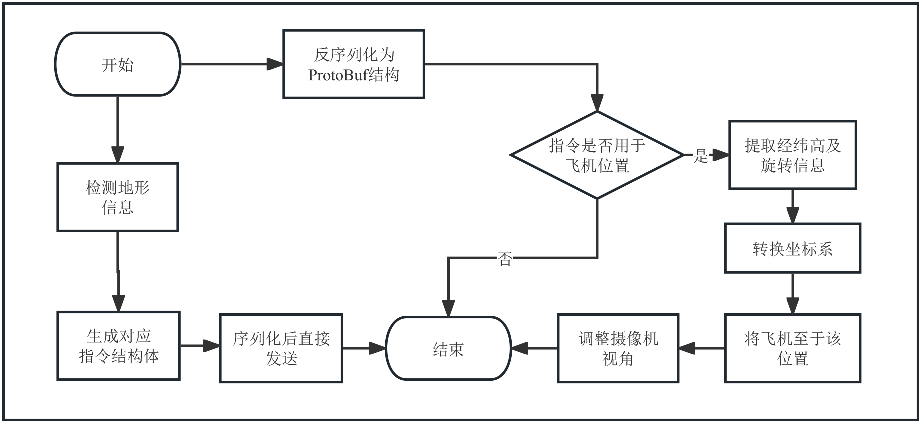
\includegraphics[width=0.8\textwidth]{pictures/flowchart4.pdf}
        \caption{飞行数据处理流程图}
        \label{module41}
    \end{center}
\end{figure}
\begin{figure}[h!]
    \begin{center}
        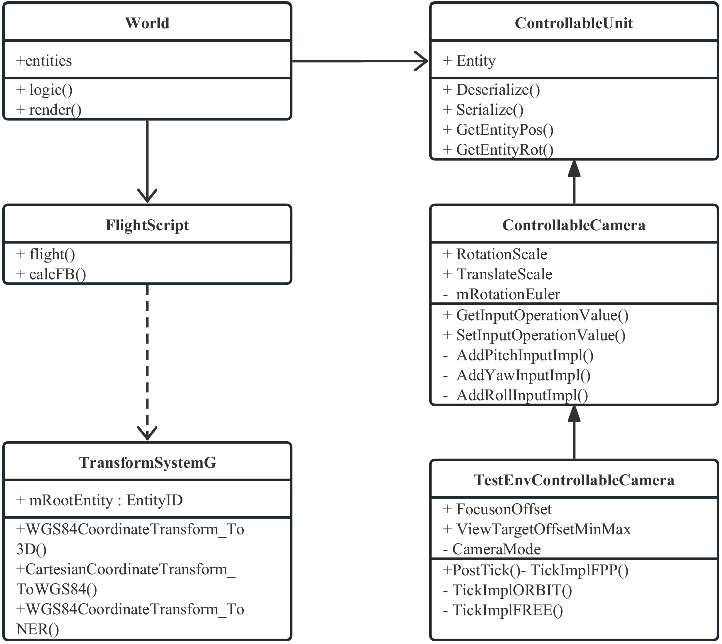
\includegraphics[width=\textwidth]{pictures/classdiagram4.pdf}
        \caption{飞行数据处理核心类图}
        \label{module42}
    \end{center}
\end{figure}
\section{本章小结}
按照软件开发的一般步骤,本章详细介绍了视景系统中数据交换子系统
的需求分析与设计过程。首先,对于整个视景系统的工作流程给出了整体说明。
其后,对数据交换子系统进行了需求分析,明确功能性需求和非功能性需求,
并以用例图和用例描述表的形式给出规格说明。其次,本章给出了数据交换子系统的架构设计。
最后,本章将子系统的主要功能划分为仿真机侧数据交换模块、协议转换模块、游戏引擎侧数据交换模块和基础飞行控制模块,
以流程图和核心类图描述了对各个模块的详细设计。

\chapter{基础数据交换的详细设计与实现}
\section{仿真机侧数据交换模块}
仿真机侧数据交换模块负责虚拟仿真机与仿真机之间的交流。他们之间通过数据链路层的原始数据包进行沟通,即除去真实数据外,仅含有Mac地址等信息。因此不能依靠TCP/IP协议收发而是直接访问底层网络。
该模块会将到来的数据帧拆为指令结构体供后续使用,或者将指令结构体包装为数据帧发送给仿真机。
\subsection{流程图}
\par
本模块的主要执行流程如图\ref{module11}所示。流程分为接收消息和发送反馈消息两部分。在接收到消息后需要先读取数据帧中的指令代号信息和长度信息,如果代号已知,则截取其后对应长度的数据段即成功拆分一条仿真机指令。
由于指令代号有接近百种,项目初期只用到部分指令,对于未知的指令对应的数据段直接跳过。发送反馈消息过程中,则需要对仿真机指令添加以太网协议头部信息,并写入WinPcap的发送队列反馈给仿真机。
\begin{figure}[h!]
    \begin{center}
        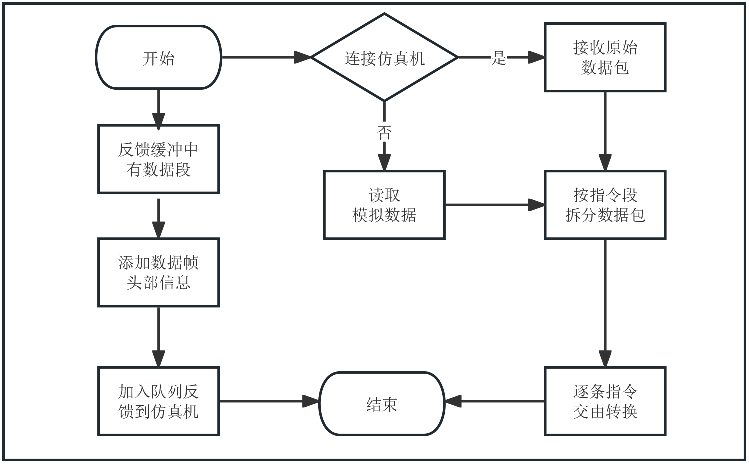
\includegraphics[width=0.8\textwidth]{pictures/flowchart1.pdf}
        \caption{仿真机侧数据交互流程图}
        \label{module11}
    \end{center}
\end{figure}
\subsection{核心类图}
\par
本模块的核心类图如图\ref{module12}所示。其中的核心是类SimulationDeviceContext,它表示仿真机与虚拟仿真机的交流环境
MacLinkCommunication类负责初始化与某一网卡设备的侦听关系,并负责数据帧的实际收取和发送。
MacReceivingRunnable是处理信息收发的线程实例,收取道德数据帧会加入接收数据帧的队列MacReceivingQueueQueue,线程实例从中取数据并交由指令转换模块。
当需要反馈时,线程实例会调用设备实例中的发送方法,最终通过MacLink实现发送。
ISimulatorDeviceInterface代表仿真机设备类的接口,其中包含了对于数据帧中指令代号的读取方法GetSimOperateCode,以及发送消息给仿真机SendToSimulationDevice方法。
CAEGenericSimulatorDeviceBase是该接口的一个实现,其代表CAE公司的仿真机设备,其中含有解读并转换该设备指令的具体算法。当需要接入其他公司设备时,
只需要重新实现SimulatorDevice接口。

\begin{figure}[h!]
    \begin{center}
        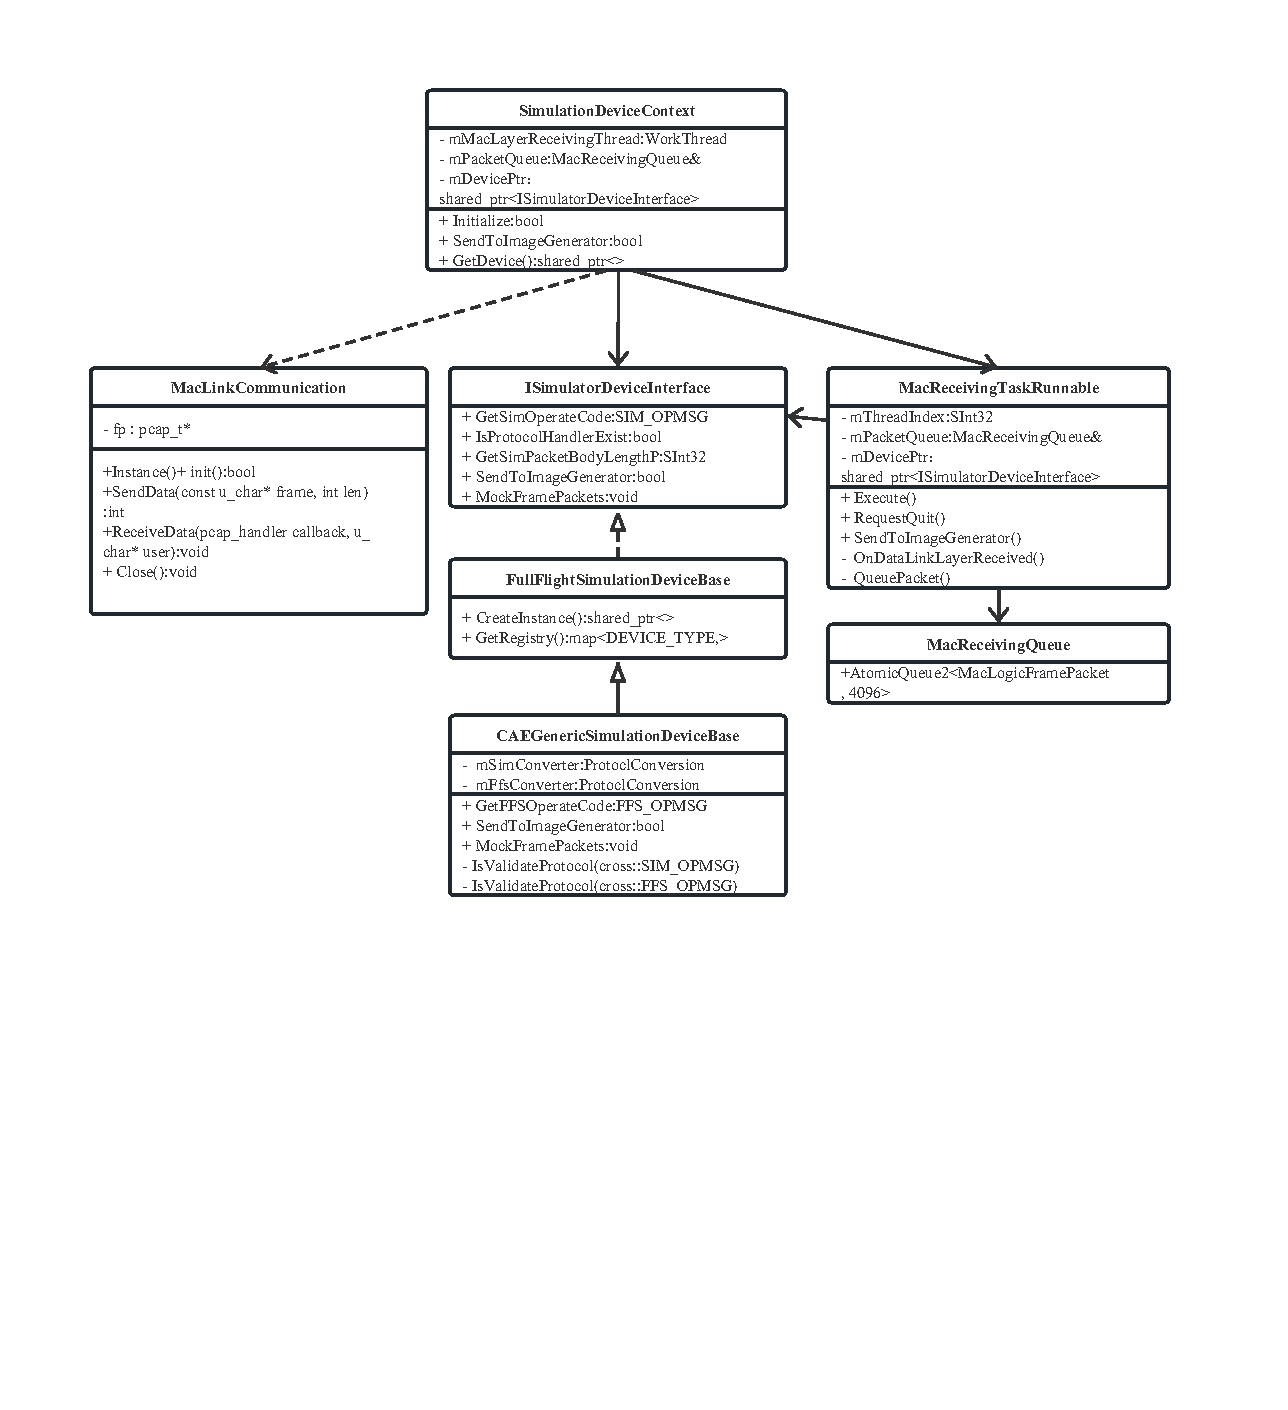
\includegraphics[width=\textwidth]{pictures/classdiagram1.pdf}
        \caption{仿真机侧数据交互核心类图}
        \label{module12}
    \end{center}
\end{figure}
\subsection{顺序图}
图\ref{seq1}是仿真机侧数据交换模块的顺序图,描述了仿真机与虚拟仿真机沟通过程中各类的交互过程。
首先交流环境类SimDeviceContext以mac地址作为参数尝试初始化MacLink,即开始侦听对应网卡设备,MacLink类中利用WinpPcap实现侦听,并判断是否侦听成功。
成功建立连接后,便可以进行数据的收发。交流环境线程MacTaskRunnable运行后会循环执行OnMacRecevied方法,
当有数据到达时会对其进行解封处理并加入MacQueue队列等待指令转换。
但有消息需要反馈时,交流环境调用线程实例的send方法,线程实例调用具体设备实例的send方法,而设备实例最终通过MacLink对象实现发送。
\begin{figure}[h!]
    \begin{center}
        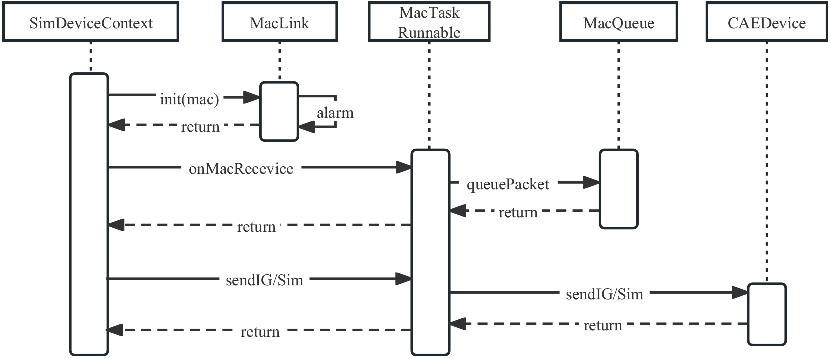
\includegraphics[width=\textwidth]{pictures/sequence1.pdf}
        \caption{仿真机侧数据交换顺序图}
        \label{seq1}
    \end{center}
\end{figure}
\subsection{关键代码}
虚拟仿真机与仿真机间通过数据链路层数据帧直接交换信息,首先要建立连接。类SimulationDeviceContext表示在虚拟仿真机中与仿真机交流的环境,Initialize函数表示了该环境的初始化流程。
代码中用到了条件编译,即根据编译时的参数来编译不同部分的代码。条件MOCKSIM表示是否使用模拟数据。如果编译时带有该参数,那么需要去读取配置文件中的模拟数据文件路径;
否则进一步与真实仿真机建立真实链路层连接。两种方式都需要启动新的线程负责消息的收发工作。
\begin{figure}[h!]
    \centering
     \lstinputlisting[basicstyle= \zihao{6}]{pictures/code1.txt}
    \caption{仿真机环境初始化代码}
    \label{code1}
\end{figure}

\par
真实链路层连接的建立则是使用到WinPcap。在Init方法中,首先通过pcap\_findalldevs方法获得该机器中所有网卡的信息,用户需要根据打印的信息选择需要使用的网卡。
之后使用pcap\_open\_live获得该网卡数据包捕获描述字,成功后即表明完成初始化link layer句柄,虚拟仿真机与仿真机可以通过用户选择的网卡进行交流。
最后通过pcap\_freealldevs释放网卡数据列表。

\begin{figure}[h!]
    \centering
     \lstinputlisting[basicstyle= \zihao{-5}]{pictures/code2.txt}
    \caption{链路层连接建立代码}
    \label{code2}
\end{figure}

\par
WorkerThread是一个由线程定义与线程实例组成的结构体。上文中提到,根据条件编译结果,会得到与仿真机或模拟数据交流的两种线程定义,
CreateRunnableThread负责根据编译情况创建工作线程,图\ref{code3}工作线程mMacLayerThread,作为与仿真机交流环境中的线程。
\begin{figure}[h!]
    \centering
     \lstinputlisting[basicstyle= \zihao{-5}]{pictures/code3.txt}
    \caption{创建工作线程代码}
    \label{code3}
\end{figure}

\par
如图\ref{code4}中第一段代码所示,原始数据包接收线程启动后,会在收到结束请求前循环执行ReceiveData方法收取数据。该方法中含有回调函数OnDataLinkReceived,用于进一步处理接收到的原始数据包,其实现如第二段代码所示。
该回调函数中会将原始数据包中的多条指令拆开,并将每段指令依次存入集合framePackets中。最后调用QueuePacket函数将该集合加入仿真机消息接收队列中。
\begin{figure}[h!]
    \centering
     \lstinputlisting[basicstyle= \zihao{-5}]{pictures/code4.txt}
    \caption{原始数据包接收代码}
    \label{code4}
\end{figure}

\par
如图\ref{code5}所示。原始数据包的解析逻辑位于方法OnDataLinkLayerReceived中。由于原始数据包是数据链路层消息,其带有数据帧头、厂商自定义信息头等数据头部信息,拆分指令段前指针cursor需要先通过ParseMacLinkLayerHeader方法跳过该部分内容,进入正式数据部分。
该部分中含有多条指令,每条指令头部有其长度信息,指针需要按照读取到的长度将数据部分进行拆分,并将指令内容复制到MacEncodingPacket对象中,加入上述仿真机消息接收队列中。虚拟仿真机从仿真机接收消息的过程就此结束。
\par
在真实的飞行训练中虚拟仿真机自然要与仿真机进行直接沟通,但在没有仿真机的开发环境中,虚拟仿真机也需要能够读取模拟数据来驱动视景系统运行。
在编译项目时将条件设置为使用模拟数据,便可以开启该流程。
\par
图\ref{code6}是处理模拟数据的实现。设备指针mDevicePtr调用MockFramePacket方法读取csv文件,ConvertCsv函数将16进制字符两两一组转换为字节内容,最后将读取到的内容转换为MacEncodingPacket类型加入仿真机消息接收队列,此部分与连接仿真机时的过程相同。读取csv文件使用到了第三方库rapidcsv。
NextCurrentFrameMockData方法中指针mCurrentCursor记录了当前读取到的csv文件行数,每次被调用都会从当前位置读取下一行数据内容。
其中,mDocument表示csv文件对象,GetRow方法可以将csv中的一行内容读取到一个vector对象中。随后会根据读取到的指令代号调用相应的转换方法ConvertCsv,把vector对象转换为指令结构体。
\begin{figure}[h!]
    \centering
     \lstinputlisting[basicstyle= \zihao{6}]{pictures/code5.txt}
    \caption{原始数据包解析代码}
    \label{code5}
\end{figure}
\begin{figure}[h!]
    \centering
     \lstinputlisting[basicstyle= \zihao{6}]{pictures/code6.txt}
    \caption{模拟数据处理代码}
    \label{code6}
\end{figure}

\par
第三章需求部分提到,视景系统会给仿真机反馈信息,该消息同样需经过虚拟仿真机,将TCP消息最终转换为原始数据包进行发送。在仿真机交流环境中SendToSimulationDevice方法负责反馈信息,即将指令结构体转换为原始数据包后发送,其调用上文中的工作线程下的同名方法,由该线程负责执行工作。
最终的实现方法则在具体的设备中,因为不同厂商的仿真机使用的数据组织结构大有不同,此处列出了为适配CAE公司仿真机而编写的方法。
\begin{figure}[h!]
    \begin{center}
        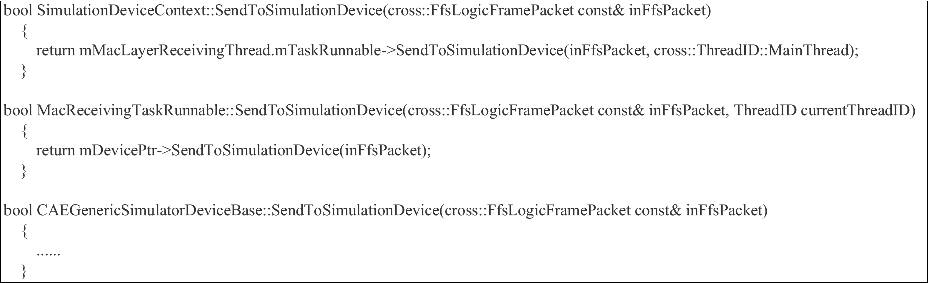
\includegraphics[width=\textwidth]{pictures/code8.pdf}
        \caption{反馈消息逻辑}
    \end{center}
\end{figure}
\par
从视景系统中来的反馈信息类型为FfsLogicFramePacket,需要将其最终封装为数据帧发送。首先需要获取其中的指令代号,调用对应指令的转换方法,若暂时无法理解该指令便产生警告。
其次需要为该数据帧添加仿真机规定的头部和尾部信息,最后通过MacLinkCommunication单例中的SendData完成数据链路层信息的发送。
\par
在使用模拟数据的情况下,如图\ref{feedbackmock}对于信息反馈只要解析其中的指令代号并打印日志即可。
\begin{figure}[h!]
    \begin{center}
        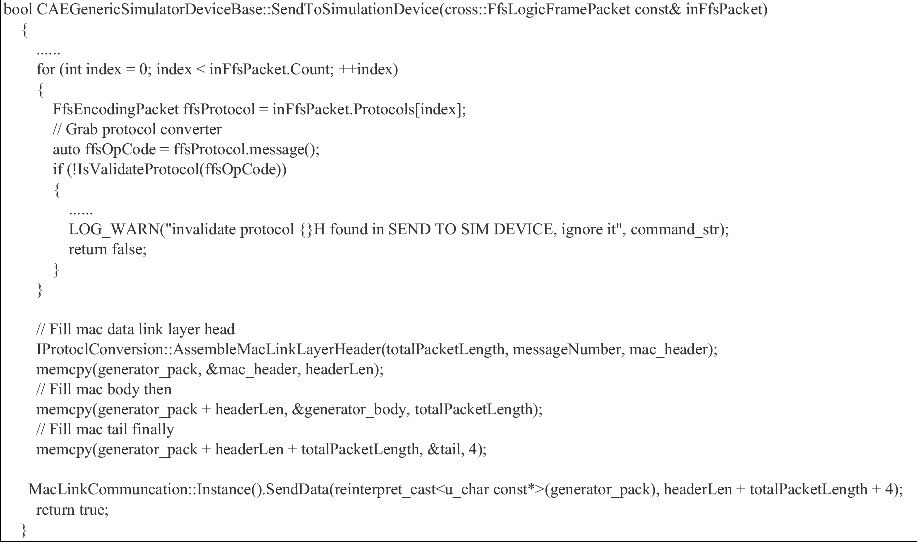
\includegraphics[width=\textwidth]{pictures/code9.pdf}
        \caption{反馈消息实现代码}
    \end{center}
\end{figure}

\begin{figure}[h!]
    \begin{center}
        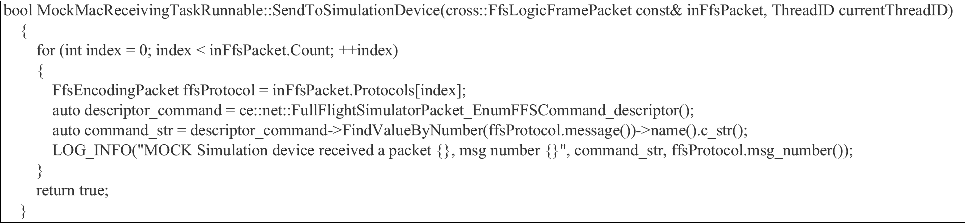
\includegraphics[width=\textwidth]{pictures/code10.pdf}
        \caption{模拟数据下反馈}
        \label{feedbackmock}
    \end{center}
\end{figure}
\par
CAEGenericSimulatorDeviceBase中的构造函数里进行了注册convert
不同厂商的仿真机厂商对于数据包中字段组成和属性编排有明显差异。如表\ref{simsattr}中对比了CAE公司和波音公司模拟机对于飞机移动这一指令数据包中的情况。
通过对比可知,首先他们的头部信息存在差别;其次虽然这一数据包中都含有经纬度、海拔高度和欧拉角信息,但他们的排列顺序明显不同;最后,对于同一个属性如Altitude长度不同,存在精度上的差异。
这些差异最终需要重新解释为统一格式以实现通用化。如图\ref{classtmp}中的代码所示,SD\_PACKET\_21H便是一个统一后用于表示飞机飞行数据的指令结构体。其中包含了基本的飞行用属性。适配新的仿真机只需要重新编写对数据包的解析函数。
\begin{table}[htbp]
    \begin{center}
        \caption{不同仿真机字段比较}
        \label{simsattr}
        \renewcommand\arraystretch{1.2}
        \begin{tabularx}{\textwidth}{ 
            | >{\centering\arraybackslash\hsize=\hsize\linewidth=\hsize}X 
            | >{\centering\arraybackslash\hsize=\hsize\linewidth=\hsize}X 
            | >{\centering\arraybackslash\hsize=\hsize\linewidth=\hsize}X 
            | >{\centering\arraybackslash\hsize=\hsize\linewidth=\hsize}X 
            | }
            \hline
            \textbf{CAE字段} & \textbf{长度} & \textbf{Boeing字段} & \textbf{长度}\\
            \hline
            OpCode & 16bit & Packet ID & 16bit\\
            \hline
            CS number & 32bit & Entity ID & 16bit\\
            \hline
            Latitude MSW & 32bit & Roll & 32bit\\
            \hline
            Latitude LSW & 32bit & Pitch & 32bit\\
            \hline
            Longitude MSW & 32bit & Yaw & 32bit\\
            \hline
            Longitude LSW & 32bit & Latitude MSW & 32bit\\
            \hline
            Altitude& 32bit & Latitude LSW & 32bit\\
            \hline
            Roll & 32bit & Longitude MSW & 32bit\\
            \hline
            Pitch& 32bit & Longitude LSW & 32bit\\
            \hline
            Yaw & 32bit & Altitude & 64bit\\
            \hline
            etc. & & etc. & \\
            \hline
        \end{tabularx}
    \end{center}
\end{table}
\begin{figure}[h!]
    \begin{center}
        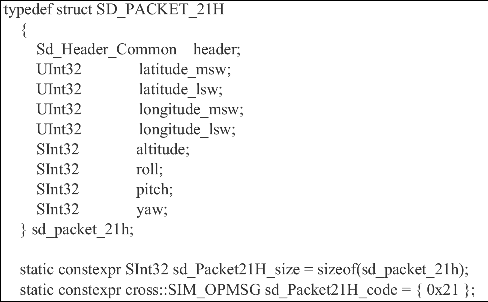
\includegraphics[width=0.8\textwidth]{pictures/code12.pdf}
        \caption{转换类模板代码}
        \label{classtmp}
    \end{center}
\end{figure}

\section{指令转换模块}
指令转换模块负责仿真机指令与自定义指令之间的转换。经过转换后的指令才能被对方理解并使用。首先仿真机指令中对于浮点数的表达方式是由该厂商自行设计的,对于不同用途不同精度要求的数据其数字表示方式均存在差异。
因此这两种结构之间的转换需要严格依照设计文档中的说明设计转换算法,而不是简单的赋值。
其次仿真机指令中最重要的无疑是关于飞机位置和姿态的指令,但由仿真机给出的位置是由经纬度高度组成的数据,而图像生成器中使用的坐标系是笛卡尔坐标系,必须经过坐标系的转换才能使用该信息。
\subsection{流程图}
\par
本模块的主要执行流程如图\ref{module21}所示。
当收到来自仿真机的指令段时,数据转换模块先根据指令代号确定指令类型,用对应的仿真机指令结构体实现反序列化,再根据指令代号查找出对应的转换器,该转换器中的转换方法可将该指令转换为对应的自定义指令。
当收到自定义指令时,同样根据指令类型查找相应的转换器,使用该转换器中的方法完成转换。
\begin{figure}[h!]
    \begin{center}
        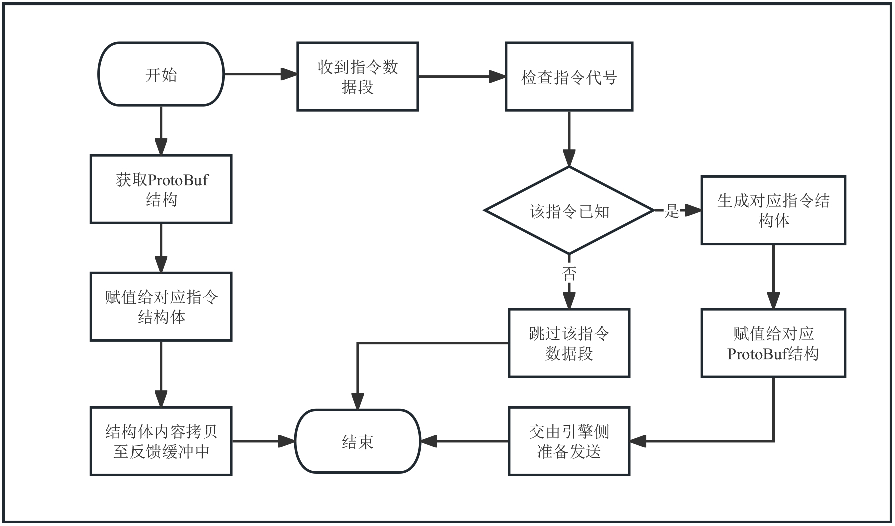
\includegraphics[width=0.8\textwidth]{pictures/flowchart2.pdf}
        \caption{数据转换流程图}
        \label{module21}
    \end{center}
\end{figure}
\subsection{核心类图}
\par
本模块的核心类图如图\ref{module22}所示。其中核心为IProtoclConversion接口,该接口中声明了仿真机指令与自定义指令间转换的方法Convert。需要注意的是在接口的实现中只需要实现其中一个方向的转换,因为一种指令只可能由仿真机给图像生成器或由图像生成器反馈给仿真机。
在CAE仿真机类中使用map存储这些转换器,表示这些转换器是专用于CAE仿真机指令的转换,如果需要接入其他仿真机则需要实现对应的转换器。
ProtoclConversion是一个模板类,成员属性T表示一个仿真机指令,成员属性F表示一个自定义指令,T和F组成互相转换的一对。
IGCommand是自定义指令类,SimCommand是仿真机指令类,真正的Convert实现在仿真机指令类中。
\par
当调用实例化模板类中的Convert方法时,该方法会调用对应指令的Convert方法。
这样设计的原因是当增加仿真机指令类型时不用考虑编写对应的转换器,为协同开发带来便利。

\begin{figure}[h!]
    \begin{center}
        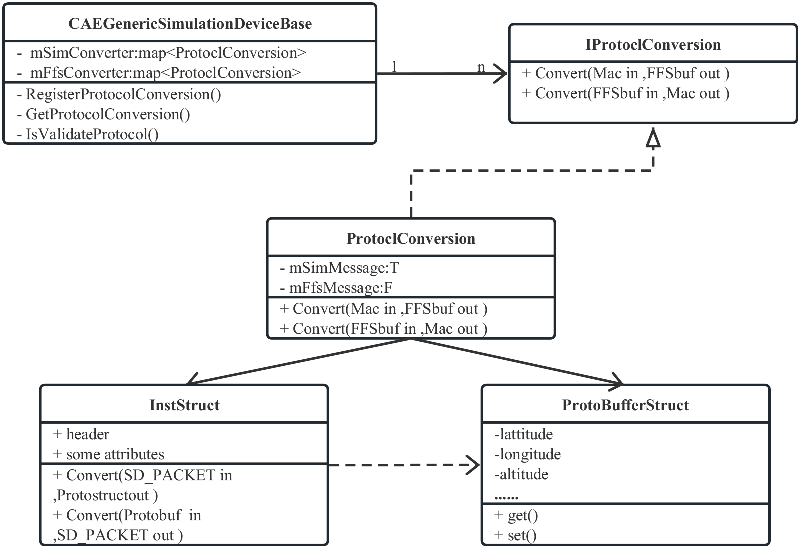
\includegraphics[width=\textwidth]{pictures/classdiagram2.pdf}
        \caption{指令转换核心类图}
        \label{module22}
    \end{center}
\end{figure}
\subsection{顺序图}
图\ref{seq2}是协议转换模块的顺序图。描述了仿真机指令与自定义指令的转换中各类的交互过程。
在系统启动后,CAEDevice的构造函数会完成所有转换器的注册,即将指令代号与指令转换器作为键值对加入map中。
在指令转换前,需要先通过指令代号到map中获取对应的转换器。
调用实例化转换器中的Convert方法时,该方法会调用到仿真机指令中的Convert实现方法。
\begin{figure}[h!]
    \begin{center}
        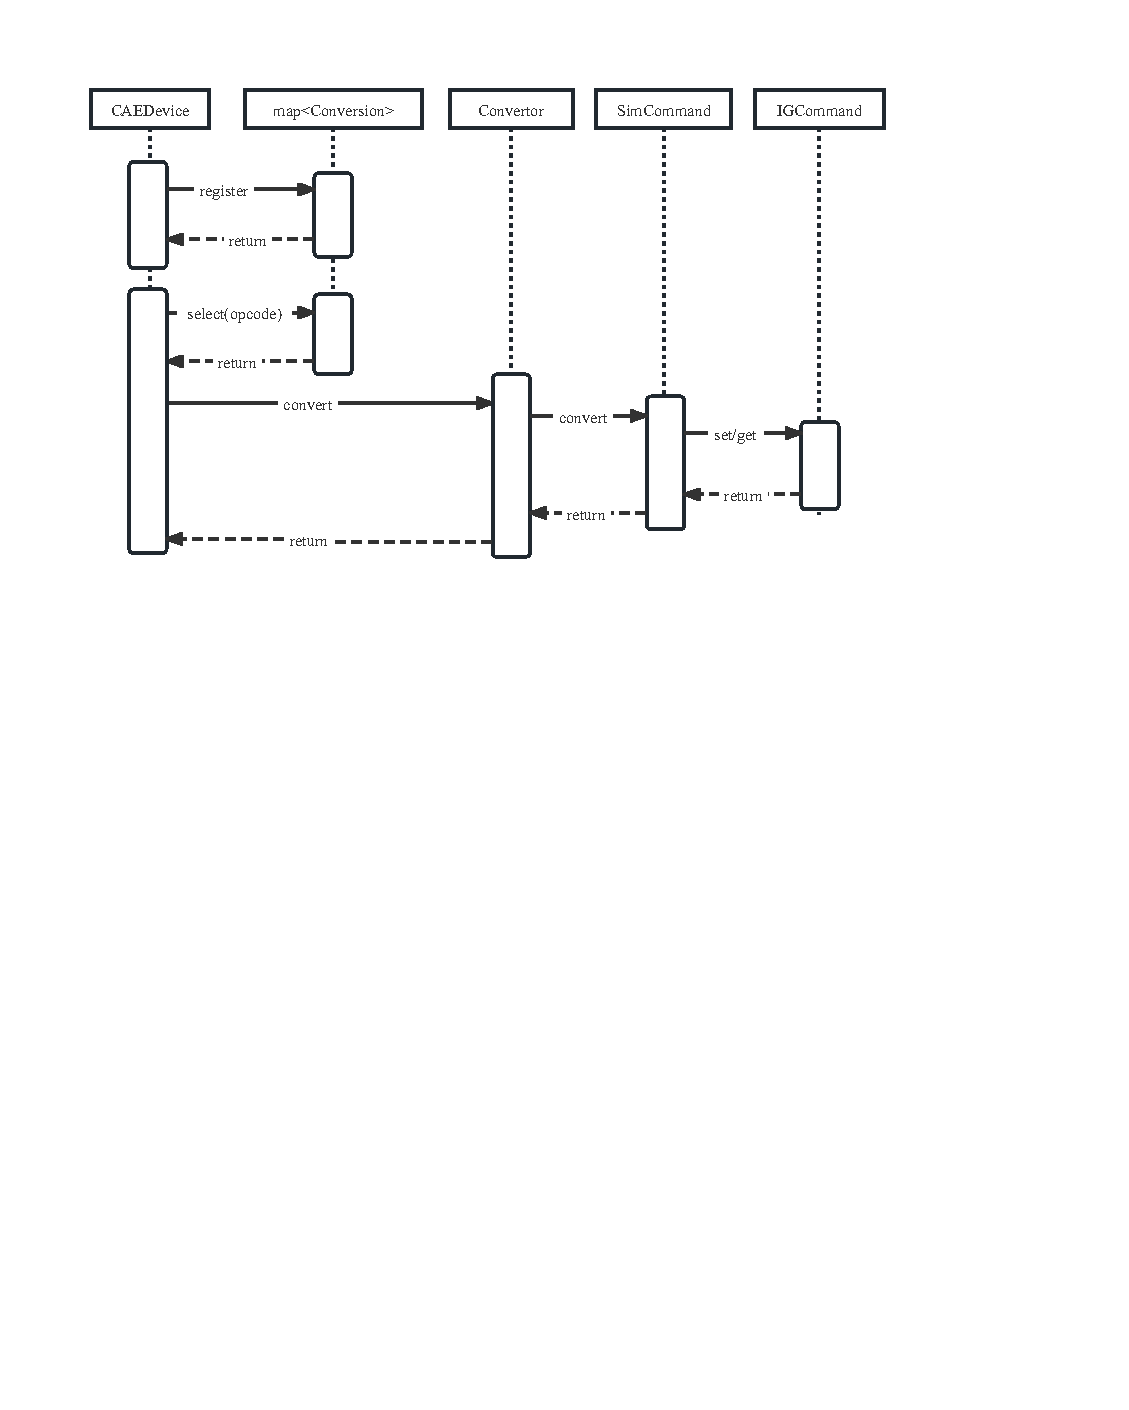
\includegraphics[width=\textwidth]{pictures/sequence2.pdf}
        \caption{指令转换顺序图}
        \label{seq2}
    \end{center}
\end{figure}
\subsection{关键代码}
使用ProtoBuffer首先需要编写一个proto文件定义程序中需要处理的结构化数据,在ProtoBuffer的术语中,结构化数据被称为Message。
如图\ref{pb21}中的代码,定义了一个名为GeodeticCSUpdate的结构化数据,其中的成员为飞机飞行所需属性,且每一个成员均被赋予唯一的编号,在编码时使用该编号表示该成员。

\begin{figure}[h!]
    \begin{center}
        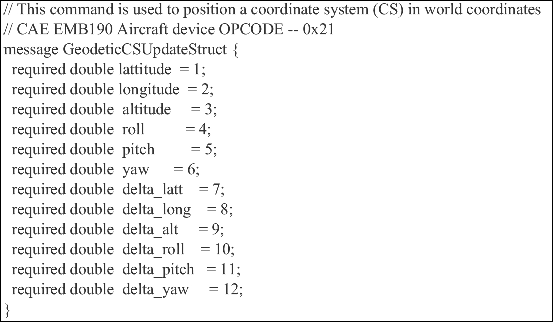
\includegraphics[width=0.8\textwidth]{pictures/code15.pdf}
        \caption{ProtoBuffer结构}
        \label{pb21}
    \end{center}
\end{figure}
\par
写好proto文件之后就可以用ProtoBuffer编译器将该文件编译成目标语言。编译为C++后会得到.pb.h和.pb.cc文件,分别为该类的头文件和实现文件,
提供了一系列的get/set函数用来修改和读取结构化数据中的数据成员。当需要将该结构化数据序列化时,类中已经提供相应的方法来把复杂的数据变成字节序列。
对想要读取数据的程序来说,也只需要使用类中的相应反序列化方法来将这个字节序列重新转换为结构化数据。

\par
系统在需要转换的时候总要根据指令代号来确定对应的转换方法,便要求在系统运作前完成对于这些转换执行者的注册。
如图\ref{convtmp}所示,类ProtoclConversion是转换执行者,这是一个模板类。T代表一个指令结构体,如上文中的SD\_PACKET\_21H;F代表一个ProtoBuffer结构如GeodeticCSUpdate。
如果指令代号为21H,则使用对应的转换执行对象里的Convert方法即可实现转换。
\begin{figure}[h!]
    \begin{center}
        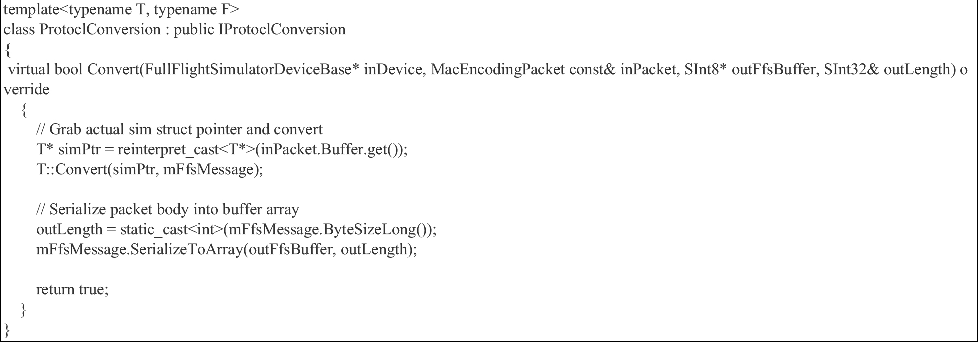
\includegraphics[width=\textwidth]{pictures/code13.pdf}
        \caption{转换执行模板类}
        \label{convtmp}
    \end{center}
\end{figure}
\par
对于一系列ProtoclConversion对象的注册代码如图\ref{regiconv}所示。转换执行者分为两组,一组为mSimConverter,根据仿真机侧的指令代号找到转换执行者;另一组为mFfsConverter,可以根据引擎侧的指令代号找到转换执行者。
RegisterProtocolConversion函数负责将执行者加入两个map中,key为指令代号,value为转换执行者的指针。此函数会在整个环境的构造函数中被多次调用,完成所有注册。
\begin{figure}[h!]
    \begin{center}
        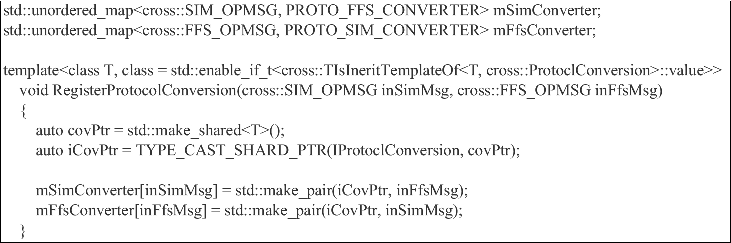
\includegraphics[width=0.9\textwidth]{pictures/code14.pdf}
        \caption{转换执行类注册代码}
        \label{regiconv}
    \end{center}
\end{figure}
\section{图像生成器侧数据交换模块}
游戏引擎侧数据交换模块负责虚拟仿真机与游戏引擎之间的交流。其利用Tbuspp插件使用TCP消息沟通,数据交换协议则是ProtoBuffer。再发送给游戏引擎的过程中,需要将发送频率的固定,因此该线程会以固定的频率被唤醒。
\subsection{流程图}

本模块的主要执行流程如图\ref{module31}所示。当发送队列中有消息时,若可以进行发送则直接发送,否则要等待新的发送时机。反馈消息接收时则不需考虑频率,直接接收消息并给到协议转换模块。
\begin{figure}[h!]
    \begin{center}
        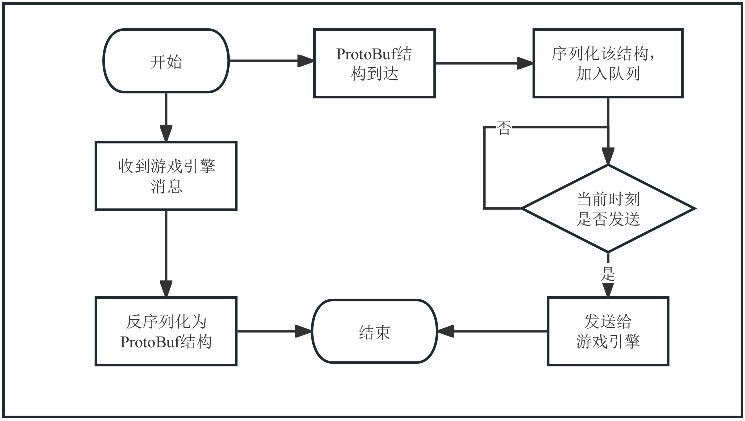
\includegraphics[width=0.8\textwidth]{pictures/flowchart3.pdf}
        \caption{图像生成器侧数据交互流程图}
        \label{module31}
    \end{center}
\end{figure}
\subsection{核心类图}

本模块的核心类图如图\ref{module32}所示。其中的核心是类ImageGeneratorContext,它表示在虚拟仿真机中与游戏引擎交流的环境,其中包含控制信息收发的线程和信息队列。
IImageGeneratorDeviceInterface则是与游戏引擎交流的接口,其中包含了对于ProtoBuffer结构中指令代号的读取方法GetOperateCode,以及发送消息给游戏引擎SendToImageGenerator方法。
FullFightSimulatorDeviceBase是对该接口的实现,其依赖控制发送频率的类FrameSynchronization。CAEGenericSimulatorDeviceBase代表CAE公司FFS设备,其中含有与该公司设备进行沟通的具体方法。
\begin{figure}[h!]
    \begin{center}
        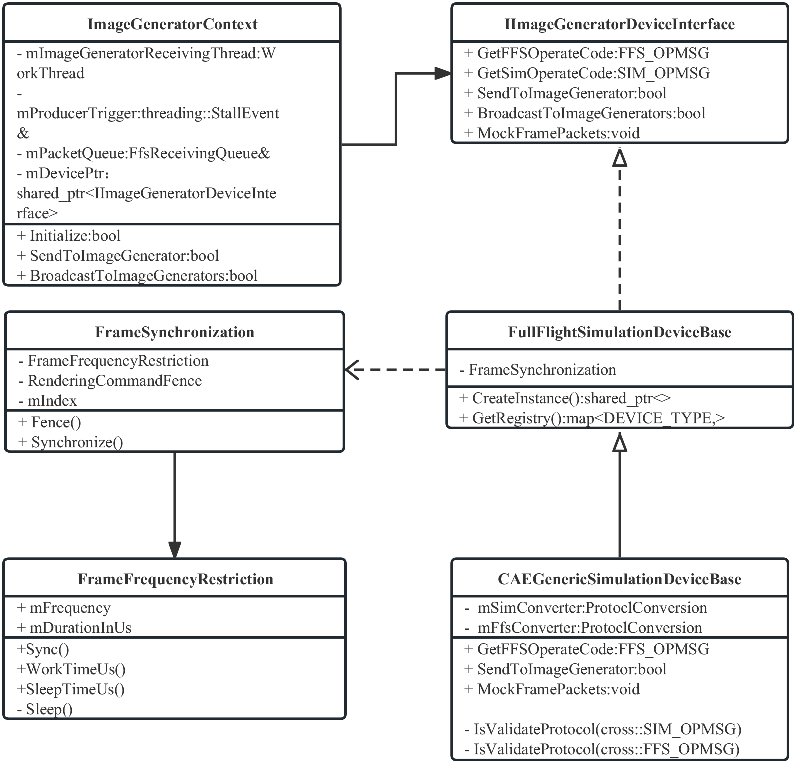
\includegraphics[width=\textwidth]{pictures/classdiagram3.pdf}
        \caption{视景系统侧数据交互核心类图}
        \label{module32}
    \end{center}
\end{figure}
\subsection{顺序图}
图\ref{seq3}是游戏引擎侧数据交换模块的顺序图。描述了虚拟仿真机与游戏引擎间沟通时各类的交互过程。
首先交流环境IGContext先通过Tbuspp的配置文件建立连接,Tbuspp插件类会判断连接是否成功。
连接建立后,交流环境通过send方法通知FFSDevice已有数据准备好发送,此时FrameSync类会介入判断在规定发送频率下此时是否可以发送。
到达发送时间后,会调用IGDevice中的send方法执行具体发送动作。
\begin{figure}[h!]
    \begin{center}
        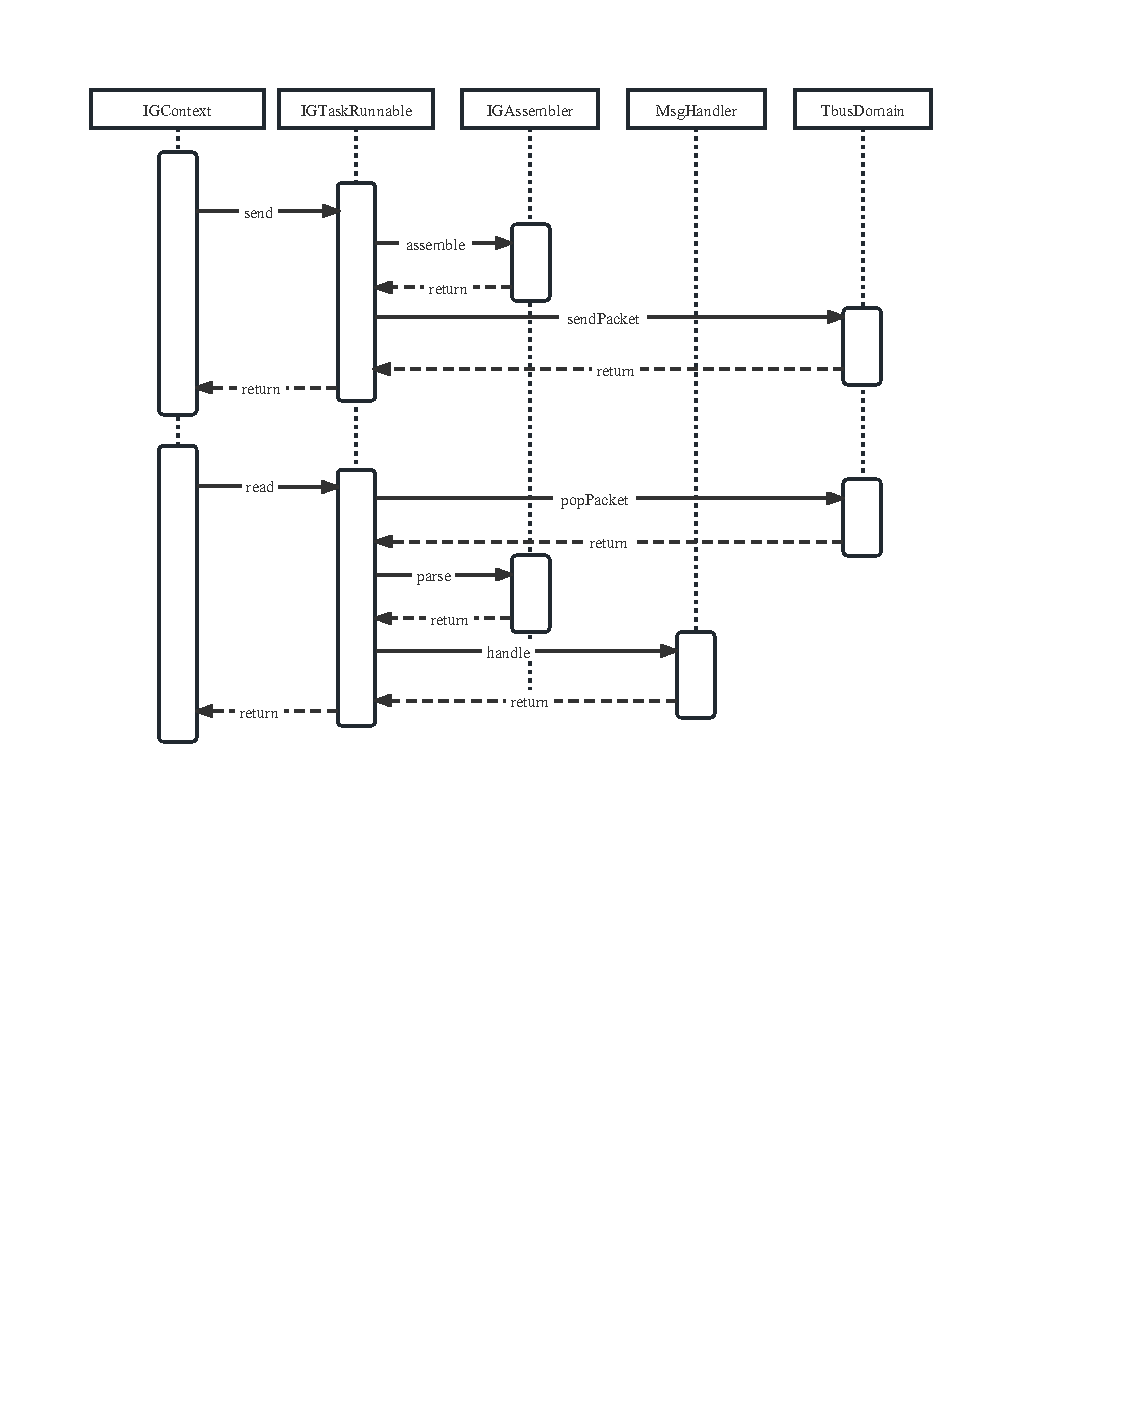
\includegraphics[width=\textwidth]{pictures/sequence3.pdf}
        \caption{游戏引擎侧数据交换顺序图}
        \label{seq3}
    \end{center}
\end{figure}
\subsection{关键代码}
虚拟仿真机与游戏引擎之间通过Tbuspp插件进行信息交流,第一步是要先建立连接。类ImageGeneratorContext表示在虚拟仿真机中与游戏引擎交流的环境,Initialize函数表示了该环境的初始化流程。
代码中同样用到了条件编译。条件MOCKIG表示不与游戏引擎建立真实连接,而是直接读取配置文件中的模拟数据文件路径,模仿视景系统给到的反馈,暂时该功能并未投入使用;
否则进一步与游戏引擎建立连接。两种方式都需要启动新的线程负责消息的收发工作。
\begin{figure}[h!]
    \begin{center}
        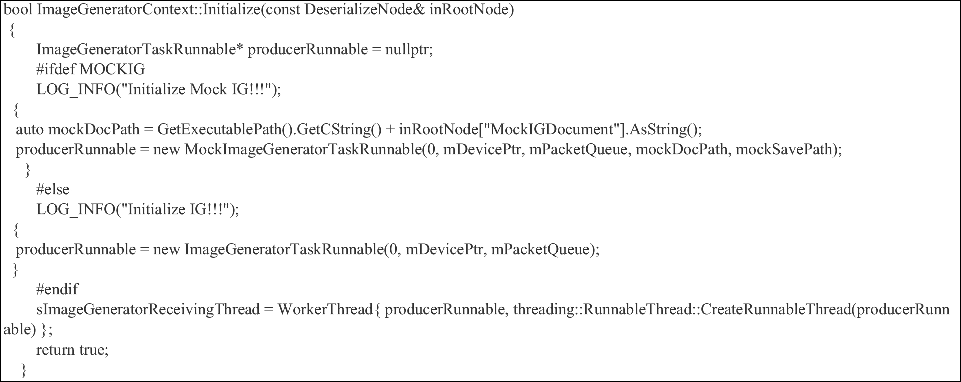
\includegraphics[width=0.9\textwidth]{pictures/code17.pdf}
        \caption{引擎侧环境初始化代码}
    \end{center}
\end{figure}
\par
Tbuspp连接的建立首先需要编写一个简单的配置文件,其中需要给出每个节点的url和busid。如图\ref{tbusconfi}中所示,VSD节点表示虚拟仿真机,另外还包含有两个视景节点,ImageGeneratorGroup则代表所有的视景节点,
当需要广播消息时可以给到该节点。此处的url均为本地地址,实际运行中,虚拟仿真机与视景系统运行在不同机器上,需根据实际情况进行配置。
\par
在Tbuspp初始化方法中,node参数表示已经过反序列化的配置文件内容,首先通过LoadDomainConfig读取所有的节点;其次通过SetLocalClient设置本地的服务节点,在虚拟仿真及侧该节点为VSD。之后使用tbuspp\_open方法开启连接,
并检查连接状态是否正常。随后获取消息的接收和发送队列in\_queue和out\_queue并对他们进行一次清空操作,做好收发消息的准备。

\begin{figure}[h!]
    \begin{center}
        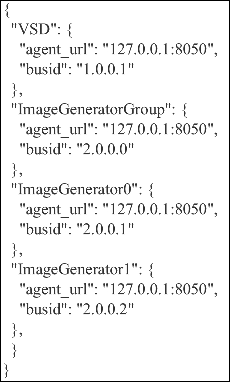
\includegraphics[width=0.3\textwidth]{pictures/code18.pdf}
        \caption{Tbuspp配置文件}
        \label{tbusconfi}
    \end{center}
\end{figure}
\begin{figure}[h!]
    \begin{center}
        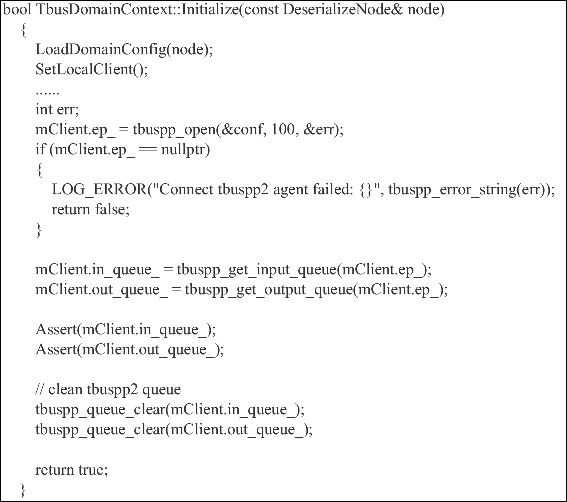
\includegraphics[width=0.8\textwidth]{pictures/code19.pdf}
        \caption{Tbuspp初始化代码}
    \end{center}
\end{figure}
\par
SendToImageGenerator方法负责发送信息至游戏引擎。其参数包括需要发送的数据和接收数据的视景系统节点名称。使用SerializeToArray方法对待发送数据进行序列化后,便交由TbusDomainContext单例处理发送操作。
其中先根据节点名称确定发送的目标节点,之后通过tbuspp\_queue\_write方法将发送内容写入本地服务节点的发送队列out\_queue中,由Tbuspp完成发送。
\begin{figure}[h!]
    \begin{center}
        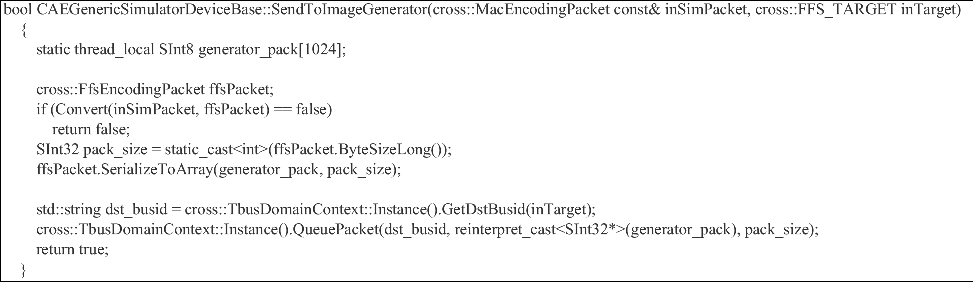
\includegraphics[width=0.9\textwidth]{pictures/code20.pdf}
        \caption{引擎侧发送信息代码}
    \end{center}
\end{figure}
\begin{figure}[h!]
    \begin{center}
        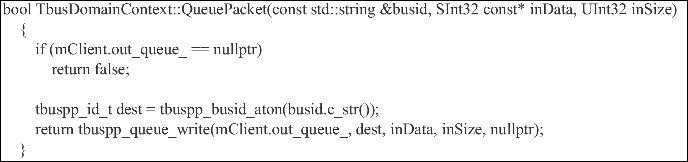
\includegraphics[width=0.8\textwidth]{pictures/code21.pdf}
        \caption{Tbuspp发送信息代码}
    \end{center}
\end{figure}
\par
在游戏中逻辑线程负责数据的产生,渲染线程负责根据数据渲染画面,一般比逻辑线程慢许多。因为逻辑线程跑的太快基本没有意义,还会耗光内存。因为逻辑线程不断的产生数据传递给渲染线程,如果渲染线程消费数据远远慢于产生数据,就会有越来越多的数据存于内存中。
因此需要对逻辑线程做出一定限制,不能让其一直保持工作状态。
\par
在本系统中对于仿真机数据的处理和传输可以认为是逻辑线程的工作,而游戏引擎部分基本为渲染线程的工作。图\ref{sync}是对于逻辑线程进行限制的核心方法Sync。
high\_resolution\_clock是C++11中的新特性,提供的拥有最小计次周期的时钟。在本系统中以微妙作为基本周期,FrameDurationUs表示每次发送的间隔周期,如果要求为60Hz的发送频率则该值为$10^6/60$微秒。
若距离上一次发送的时间仍小于间隔周期,则使用Sleep方法将线程挂起剩余的时间长度。
\begin{figure}[h!]
    \begin{center}
        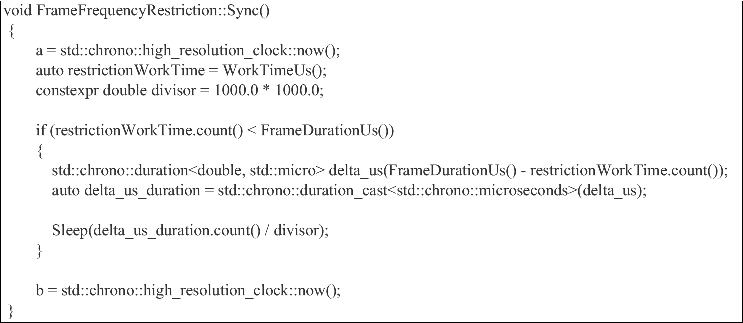
\includegraphics[width=0.8\textwidth]{pictures/code22.pdf}
        \caption{限制频率代码}
        \label{sync}
    \end{center}
\end{figure}
\par
在第二章的介绍中提到Nagle算法可以减少TCP包的个数,更高效的利用网络带宽。但同时也会带来一些延时问题,在实时交互应用中尤其重要。
对于部署虚拟仿真机和游戏引擎的Windows系统机器都需要在注册表中将TcpAckFrequency字段和TcpNoDelay字段值修改为1,以禁用Nagle算法。
\begin{figure}[h!]
    \begin{center}
        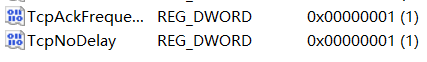
\includegraphics[width=0.8\textwidth]{pictures/nagle.png}
        \caption{Windows中禁用Nagle}
    \end{center}
\end{figure}
\section{飞行控制模块}
\subsection{顺序图}
图\ref{seq4}是飞行控制模块的顺序图,描述了游戏引擎执行飞行逻辑时各类大致的交互过程。
场景类World每帧调用tick函数执行该帧中的操作,逻辑脚本FlightScript调用引擎核心中负责变换和物理的System中的算法,完成飞机的移动旋转,以及对于下方地形的检测。
Camera类也会被World每帧调用,执行不同视角逻辑下的移动旋转,变焦等动作。
\begin{figure}[h!]
    \begin{center}
        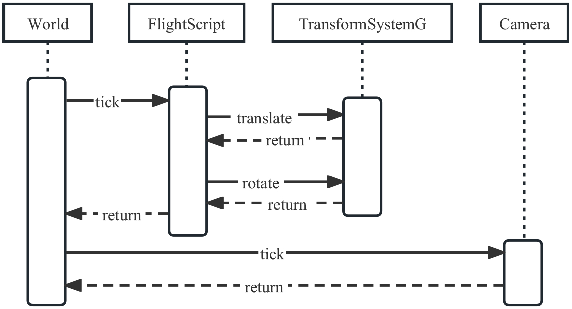
\includegraphics[width=.8\textwidth]{pictures/sequence4.pdf}
        \caption{飞行控制顺序图}
        \label{seq4}
    \end{center}
\end{figure}
\subsection{飞行位置与姿态计算}
由经度longitude,纬度latitude和高度altitude组成的LLA坐标系,可以说是最为广泛应用的一个地球坐标系,它给出一点的大地纬度、大地经度和大地高程直观地告诉我们该点在地球中的位置,故又被称作经纬高坐标系。仿真机给出的飞机位置便是LLA坐标形式。
地心地固坐标系ECEF是以地心为原点的笛卡尔坐标系,在游戏引擎中自然使用该坐标系更为便捷。在两种坐标系下地球都是默认为两级略扁的规则椭球形,赤道长半轴为6378137.0米,两极短半轴为6356752.314245米,扁率为1/298.257223563。
B. R. Bowring在1985年便提出了两种坐标间的转换方法\cite{cha4}。如图\ref{lla2ecef}和图\ref{ecef2lla}所示。其中a为长半轴,b为短半轴,e为椭球的偏心率,N为椭球的曲率半径。
$$e^2=\frac{a^2-b^2}{a^2}$$
$$N=\frac{a}{\sqrt{1-e^2sin^2(lat)}}$$

\begin{figure}[h!]
    \begin{center}
        \includegraphics[width=0.8\textwidth]{pictures/code23.pdf}
        \caption{LLA转换为ECEF坐标代码}
        \label{lla2ecef}
    \end{center}
\end{figure}

\begin{figure}[h!]
    \begin{center}
        \includegraphics[width=0.8\textwidth]{pictures/code28.pdf}
        \caption{ECEF转换为LLA坐标代码}
        \label{ecef2lla}
    \end{center}
\end{figure}
\par 
除了LLA与ECEF之间的转换,我们还需要建立一个东北天坐标系ENU,这是一个在物体所在位置建立的坐标系,三个轴分别指向东方,上方和北方。飞机的欧拉角便是以ENU坐标系为初始状态进行旋转。
我们依旧可以仅从LLA坐标得到ENU坐标系。如图\ref{llanue}所示,我们可以根据经度和纬度做简单的三角函数运算得出该点法线向量normal,即ENU坐标系中的up方向。同时法线与y轴所构成的平面一定与东方向垂直。
在三维向量下,两个不平行的向量进行叉乘可以得到垂直于该平面的一个向量。根据该几何意义,将normal与y轴单位向量(0,1,0)叉乘即可得到东方向。同理将东方向与normal叉乘,即可得到北方向,ENU坐标系就此构建完毕。
飞机的姿态需要使用欧拉角与ENU坐标系形成的旋转矩阵相乘,才能正确得到游戏引擎世界坐标系ECEF下的姿态。
$$normal.x=cos(lat) * sin(lon)$$
$$normal.y = sin(lat)$$
$$normal.z = -cos(lat) * cos(lon)$$
\begin{figure}[h!]
    \begin{center}
        \includegraphics[width=0.8\textwidth]{pictures/ecef.png}
        \caption{LLA与ENU坐标系}
        \label{llaneu}
    \end{center}
\end{figure}



\section{初步运行测试}
\section{本章小结}
本章在需求分析及总体设计的基础上,对系统包含的四个模块核心功能的实现做了具体阐述。对于虚拟仿真机与仿真机和游戏引擎的数据交换模块,都介绍了建立连接的过程和收发信息的过程。仿真机侧额外介绍了为应对不同厂商模拟机而做的设计,
游戏引擎侧则额外介绍了稳定信息收发帧率的实现方法。在协议转换模块中介绍了使用ProtoBuffer协议的流程方法,对较为特殊的字段转换算法做了详细说明。在最后的飞行控制模块中,介绍了让飞机飞行的实现,三种观察方式摄像机的实现,以及飞行中对于地形信息检测的实现。

\chapter{数据同步与平滑机制的设计与实现}
系统测试是为了在用户开始使用软件前,尽可能地发现软件中潜在的错误
和不合理之处,确保最后将高质量的软件交付给用户。为了验证系统的功能和
性能是否与需求分析时的规格说明一致,本章节在开发环境和真实FFS环境中分别做综合性的功能测试和性能测试。

在第二章的介绍中提到Nagle算法可以减少TCP包的个数,更高效的利用网络带宽。但同时也会带来一些延时问题,在实时交互应用中尤其重要。
对于部署虚拟仿真机和游戏引擎的Windows系统机器都需要在注册表中将TcpAckFrequency字段和TcpNoDelay字段值修改为1,以禁用Nagle算法。
\begin{figure}[h!]
    \begin{center}
        \includegraphics[width=0.8\textwidth]{pictures/nagle.png}
        \caption{Windows中禁用Nagle}
    \end{center}
\end{figure}
\section{开发PC环境测试}
由于国内的FFS全部位于航空公司的训练基地内,不具备移动的可能性,平日开发过程中的测试均使用虚拟仿真机读取模拟数据,并在开发PC上完成视景渲染。
受限于硬件性能,在开发环境下的测试以功能测试为主,确保功能正常运作即可,对于画面帧率和分辨率之类不做严格要求。
\subsection{测试环境}
在开发环境下,虚拟仿真机由笔记本电脑担任,模拟数据也位于该电脑上,在Windows系统上运行程序,便可以通过Tbuspp与视景建立连接,不断地读取并发送数据。
对于运行视景的机器有较高的硬件要求,GPU部分要使用较高型号才能让开发人员流畅的观察场景。同时由于搭载了大型机场场景数据库,对于硬盘容量也有较高要求。在测试环境的具体物理配置信息如表\ref{devhard}所示。
\begin{table}[h!]
    \begin{center}
        \caption{开发环境物理配置}
        \renewcommand\arraystretch{1.5}
        \label{devhard}
        \begin{tabularx}{\textwidth}{ 
             >{\centering\arraybackslash\hsize=.4\hsize\linewidth=\hsize}X 
             >{\centering\arraybackslash\hsize=.4\hsize\linewidth=\hsize}X 
             >{\centering\arraybackslash\hsize=\hsize\linewidth=\hsize}X 
             }
             \hline
            \textbf{设备} & \textbf{配置项} & \textbf{详情}\\
             \hline
             & CPU & AMD Ryzen 7 4700G 8-Core Processor\\
           
             & GPU & NVIDIA GeForce RTX 3060\\
             
             视景运行机 & 内存 & 32GB\\
            
             & 硬盘 & 8TB\\
             
             & 系统 & Windows 10 专业版 22H2\\
             \hline
             & CPU & AMD Ryzen 7 5800H with Radeon Graphics\\
           
             & GPU & AMD Radeon(TM) Graphics\\
             
             虚拟仿真机 & 内存 & 16GB\\
            
             & 硬盘 & 512GB\\
             
             & 系统 & Windows 10 专业版 22H2\\
             \hline
            \end{tabularx}
    \end{center}
\end{table}
\par
为了顺利运行系统,服务器上需要配置系统运行的软件环境,详细信息如表\ref{devsoft}所示。
开发PC测试环境下的软件要求与真实FFS下的测试相同,后不再赘述。两方都需要C++与Python的运行环境,且双方通过Tbuspp沟通。
在虚拟仿真机中,需要与仿真机进行直接的链路层信息交流,需使用WinPcap软件。测试环境部署配置完成后应当能保证系统不会因为环境问题出错。

\begin{table}[h!]
    \begin{center}
        \caption{开发环境软件配置情况}
        \label{devsoft}
        \renewcommand\arraystretch{1.5}
        \begin{tabularx}{0.8\textwidth}{ 
             >{\centering\arraybackslash\hsize=.5\hsize\linewidth=\hsize}X 
             >{\centering\arraybackslash\hsize=\hsize\linewidth=\hsize}X 
             }
             \hline
            \textbf{配置项 } & \textbf{详情}\\
             \hline
             C++运行环境 & VS\_C++\_MSVC\\
           
             Python运行环境 & Python\thinspace 3.10\\
             
             底层网络访问 & WinpCap\thinspace v4.1.3\\
            
             服务网格 & Tbuspp \thinspace 0.6.0\\
             \hline
            \end{tabularx}
    \end{center}
\end{table}
\subsection{功能测试}
对于本系统的功能测试而言,视景中的飞机能够按照模拟数据中的路径飞行,即可说明从数据读取到协议转换再到最后的信息发送功能都是通过测试的。
\par 
图\ref{synctest}是对频率限制工具FrameFrequencyRestriction测试的效果,测试过程中将其频率设置为30Hz,运行csv文件读取部分程序,
可以看到从读取第18行数据到读取第48行数据中正好间隔1秒钟。多种频率均能通过测试。

\begin{figure}[h!]
    \begin{center}
        \includegraphics[width=0.4\textwidth]{pictures/frame.png}
        \caption{30HZ频率限制效果}
        \label{synctest}
    \end{center}
\end{figure}
\par
我们在测试中使用到的模拟数据是飞行员在训练基地FFS上操作绕深圳宝安机场飞行一周后得到的数据。
该数据的采样频率为60Hz,共6万余组数据,每组数据中包含仿真机输出的原始经纬高和欧拉角信息。
首先测试经过虚拟仿真机发送给游戏引擎的数据是否正确,采用的方法是在GIS软件中绘制这组输出数据,查看绘制路径与飞行员的飞行路径是否相同。
图\ref{GIStrace}中的轨迹是由上述原始数据经过虚拟仿真机处理最终输出的6万个点构成,可以看到轨迹起始位置精确的位于宝安机场的跑道上,
起飞后环绕深圳市区飞行,最终截止于羊台山森林公园。与飞行员核对后确认本路径准确无误,说明由仿真机到游戏引擎中间一系列数据操作均可以通过测试。

\par
在确认虚拟仿真机输出无误后,便可使用此数据进一步测试游戏引擎中飞行控制逻辑。图\ref{firsttest}是飞机第一视角下的飞行画面,可以看到根据模拟数据,飞机准确出现在宝安机场跑道上,
且后续飞行中的爬升转向时的视角偏转完全符合实际情况,最终飞机按照轨迹终止于场景中的森林公园上空。此测试过程同样表明第一视角摄像机可以正确跟随飞机位置并做出相同的姿态。

\begin{figure}[h!]
    \begin{center}
        \includegraphics[width=.9\textwidth]{pictures/trace.png}
        \caption{GIS绘制路径}
        \label{GIStrace}
    \end{center}
\end{figure}
\begin{figure}[h!]
    \begin{center}
        \includegraphics[width=.9\textwidth]{pictures/firstcamera.png}
        \caption{飞机第一视角}
        \label{firsttest}
    \end{center}
\end{figure}
\par
当摄像机位于第一视角下,按下X键即可切换为环绕视角。如图\ref{orbittest}所示,此时摄像机不在位于驾驶舱位置,而是在一定距离外始终看向驾驶舱。
鼠标左右方向的滑动可以改变Yaw角使摄像机水平方向的环绕,上下的滑动则改变Pitch角是竖直方向的环绕。经测试操作感受与主流游戏基本一致。

\begin{figure}[h!]
    \begin{center}
        \includegraphics[width=0.9\textwidth]{pictures/orbitcamera.png}
        \caption{飞机环绕视角}
        \label{orbittest}
    \end{center}
\end{figure}
\par
当摄像机位于环绕视角下,按下X键即可切换为自由视角。如图\ref{freetest}所示,此时摄像机会在当前位置脱离飞机,并可以去到场景中的任意位置。
键盘的WASD键为前后左右移动,EQ键控制上下移动,这些移动方向都根据摄像机自身坐标系改变。Shift键则可以加速移动。经测试,操作感受与游戏引擎中的场景漫游基本一致。
\begin{figure}[h!]
    \begin{center}
        \includegraphics[width=.85\textwidth]{pictures/freecamera.png}
        \caption{自由视角}
        \label{freetest}
    \end{center}
\end{figure}
\par
飞机在飞行过程中会产生一些反馈信息,沿原路径最终送回仿真机。比如飞机在起飞和降落过程中会持续检测三个起落架的离地高度,
测试时便选用此信息,最终检查虚拟仿真机输出的原始数据包中此信息的值与训练基地FFS的反馈是否类似。
表\ref{fbcomp}对比了同一帧下CrossEngine和FFS关于起落架离地高度的反馈信息。由于地形资源存在些许差异,双方在此数据上并不会完全一致,
在合理范围内即可。
\begin{table}[h!]
    \begin{center}
        \caption{反馈信息对比}
        \label{fbcomp}
        \renewcommand\arraystretch{1.5}
        \begin{tabularx}{0.8\textwidth}{ 
             |>{\centering\arraybackslash\hsize=.7\hsize\linewidth=\hsize}X 
             |>{\centering\arraybackslash\hsize=1.15\hsize\linewidth=\hsize}X 
             |>{\centering\arraybackslash\hsize=1.15\hsize\linewidth=\hsize}X
             |
             }
             \hline 
            \textbf{起落架编号} & \textbf{CrossEngine} & \textbf{FFS}\\   
             \hline
             1 & 3.822m & 3.392m\\
             \hline
             2 & 3.787m & 3.368m\\     
             \hline
             3 & 3.787m & 3.368m\\
             \hline 
             ...& ... & ...\\
             \hline 
             1 & 40.031m & 39.894m\\
             \hline 
             2 & 39.914m & 39.785m\\
             \hline 
             3 & 39.912m & 39.785m\\
             \hline  
            \end{tabularx}
    \end{center}
\end{table}
\section{FFS环境测试}
真实FFS环境测试去到南方航空珠海基地,这里是亚洲最大,机型最全的模拟飞行训练基地,共拥有28台民航局运输司认证的最高D等级FFS,每年有超过7000名飞行员在此训练,是名副其实的中国民航飞行员培养摇篮。
在真实FFS环境中,主要对于与仿真机连接、飞机飞行等功能测试;同时对于帧率的稳定性进行测试。
\subsection{测试环境}
在真实FFS环境下虚拟仿真机与视景运行机同样位于两台电脑上,此时虚拟仿真机不再读取模拟数据,而是与仿真机进行交流,即可以接受飞行员的操作。
在硬件配置方面,基本为最新且性能最强的配件,保障视景流畅运行。在测试环境的具体物理配置信息如表\ref{ffshard}所示。

\begin{table}[h!]
    \begin{center}
        \caption{FFS环境物理配置}
        \label{ffshard}
        \renewcommand\arraystretch{1.5}
        \begin{tabularx}{\textwidth}{ 
             >{\centering\arraybackslash\hsize=.4\hsize\linewidth=\hsize}X 
             >{\centering\arraybackslash\hsize=.4\hsize\linewidth=\hsize}X 
             >{\centering\arraybackslash\hsize=\hsize\linewidth=\hsize}X 
             }
             \hline
            \textbf{设备} & \textbf{配置项} & \textbf{详情}\\         
             \hline
             & CPU & Intel® Core™ i9-12900K Processor\\
           
             & GPU & NVIDIA RTX A6000\\
             
             视景运行机 & 内存 & 64GB\\
            
             & 硬盘 & 8TB\\
             
             & 系统 & Windows 10 专业版 21H2\\
             \hline
             & CPU & Intel® Core™ i9-12900K Processor\\
           
             & GPU & Intel® UHD Graphics 770\\
             
             虚拟仿真机 & 内存 & 32GB\\
            
             & 硬盘 & 2TB\\
             
             & 系统 & Windows 10 专业版 21H2\\
             \hline
             
            \end{tabularx}
    \end{center}
\end{table}
\subsection{功能测试}
仿真机与虚拟仿真机通过网线连接。测试中启动与仿真机连接程序后,先选择要使用的网卡。连接建立成功后便可以开始正常接收数据。测试情况如图\ref{vsimcon}所示。
虚拟仿真机已成功读取到网卡上来自仿真机的原始数据包。
\begin{figure}[h!]
    \begin{center}
        \includegraphics[width=.8\textwidth]{pictures/maclink.png}
        \caption{仿真机连接}
        \label{vsimcon}
    \end{center}
\end{figure}
\par
对于数据交换相关用例的测试同样是与服役中的FFS使用同一条预设路径飞行进行对比。本次测试选择的机场为广州白云机场,路径为跑道上的起飞过程。在服役FFS中运行的视频效果如图\ref{flightffs}所示,飞机即将在白云机场02L号跑道上完成起飞。
图\ref{flightffs}则展示了本视景系统运行该路径的情况,系统可以根据仿真机的数据正确将飞机初始位置置于机场02L号跑道,且在后续起飞过程中视景画面与上述服役FFS视频中完全一致。
目前画面仍存在球幕上的畸变问题以及颜色不准确的问题,但对于数据交换系统而言已经实现了核心功能。
\begin{figure}[h!]
    \begin{center}
        \includegraphics[width=.8\textwidth]{pictures/ffs2.png}
        \caption{服役中FFS运行效果}
        \label{flightffs}
    \end{center}
\end{figure}
\begin{figure}[h!]
    \begin{center}
        \includegraphics[width=.8\textwidth]{pictures/ffs.png}
        \caption{本视景系统运行舱内效果}
        \label{flighttest}
    \end{center}
\end{figure}
\subsection{性能测试}
性能测试的部分主要测试连续运行下视景系统的帧率稳定性。帧率检测使用第三方的监控软件,连续飞行一个小时,记录平均帧率、最高帧率、最低帧率和1\% Low帧的情况。
其中最高帧率与最低帧率并不是某一时刻的帧率,而是极短时间内的平均帧率。1\% Low是选取了帧生成时间最长的1\%的帧计算的平均帧率,这些帧不一定是连续的,所以一般会低于最低帧率,
表示整段测试时间内某些时刻的剧烈帧率波动。
\par
测试结果如表\ref{frametest}所示,视景系统限制帧率上限为60FPS,平均帧率十分接近这一数值,说明总体来讲基本能达到长时间运行下的帧率要求。
最高帧率60.8FPS说明对于帧率的限制较为成功。1\%Low距离平均帧率有较大的距离,说明在某些复杂场景下会产生比较剧烈的瞬时帧率波动。
\begin{table}[h!]
    \begin{center}
        \caption{帧率测试结果表}
        \label{frametest}
        \renewcommand\arraystretch{1.5}
        \begin{tabularx}{0.8\textwidth}{ 
             |>{\centering\arraybackslash\hsize=\hsize\linewidth=\hsize}X 
             |>{\centering\arraybackslash\hsize=\hsize\linewidth=\hsize}X 
             |
             }
             \hline 
            \textbf{项目} & \textbf{数值}\\   
             \hline
             运行时间 & 3612.015s\\
             \hline
             总帧数 & 212748 Frame\\     
             \hline
             平均帧率 & 58.9 FPS\\
             \hline 
             最低帧率& 48.6 FPS\\
             \hline 
             最高帧率& 60.8 FPS\\
             \hline 
             1\% Low& 28.1 FPS\\
             \hline  
            \end{tabularx}
    \end{center}
\end{table}
\section{系统测试}
\section{本章小结}
本章首先介绍了系统测试,通过系统测试可以有效保证系统的质量,同时可以验证系统的可用性。
随后将测试分为了开发环境和真实FFS环境,分别作了部分功能测试,并由于硬件性能原因只在FFS环境中做了性能测试。
通过此测试可以证明系统满足需求分析中的功能需求,并在FFS环境中达成非功能需求。

\chapter{总结与展望}
\section{项目总结}
在国际局势紧张的大背景下,突破技术封锁愈发关键,这两年在国家紧锣密鼓的推进下各行业纷纷涌现出惊喜突破。
在关系到万家百姓出行的航空领域,我们已经拿出C919这一成果,相信不久之后便能迎来国产飞机的第一批旅客。
而在飞行训练相关的全动飞行模拟机领域仍有许多空白,能够达到训练标准的视景系统便是空白之一。
本文中描述了自主研发的全动飞行模拟机视景系统中的数据交换部分的设计与实现过程,能够让视景系统接入未开放接口的仿真机是主要工作。
\par
在项目开始阶段,本文通过结合文档和网络流量分析的方法,明确了仿真机与外界的交流方式。
仿真机中的网络协议栈最高层为数据链路层,其发出或接收的数据帧仅被以太网协议封装。
为了让其与位于应用层的视景系统沟通,系统中引入了虚拟仿真机这一角色。其首先充当仿真机侧的网络协议栈,负责接收并解封仿真机的数据帧。
其次因为双方都有自己的数字表示方法和数据组织结构,它需要对双方的数据内容进行转换。最后仿真机也负责与视景系统中的图像生成器通过TCP消息交流,将仿真机的指令送达或接收反馈指令。
在此过程中,为了尽可能提高交流效率,采用了开启立即转发模式、使用ProtoBuffer数据交换协议、禁用Nagle算法等措施。
\par
系统实现完成后进行了初步的测试,在将已被验证的多种指令给到视景系统后,其均能产生正确的对应效果。
但使用多个图像生成器进行融合投影时,发现存在两侧图像撕裂的问题。经排查原因在于多个图像生成器的数据没能同步,由此引入网络帧缓冲机制解决该问题。
之后又发现飞机在低空较高速飞行时,图像交界处存在抖动现象,经排查发现问题是多个投影仪的刷新时间没能同步。最终采用对缓冲中的数据插值的方法在软件层面缓解了该问题。
\section{项目展望}
虽然该视景系统已经达成一定的效果,但显然距离终极目标仍有距离,需要在后续的工作中安排完成。
\begin{itemize}
    \item [(1)]
    在多种仿真机适配方面虽然在系统结构上留下了空间,但实际操作比较困难。因为难以与国外FFS厂商达成合作,只能依赖现有文档去做逆向工程探索仿真机的私有协议结构与内容,这会是极其繁琐的工作。
    期待能够与未来的国产FFS厂商通力合作,不再经历如此费力的工作。
    \item [(2)]
    从整个视景系统来看,距离达到D级模拟机的标准任重道远,作为新产品必将经过严格的审查,各类灯光、天气、突发事件的模拟必须准确到位。实现上百条的细节要求仍需要整个团队相当时间的通力合作。
    \item [(3)]
    此视景系统是基于腾讯自研游戏引擎搭建,这不仅迈出国产视景系统的一步,也是又一自研引擎成长的过程,当前综合渲染效果及稳定性肯定不及成熟的商业游戏引擎。随着该游戏引擎的逐步完善,整个视景系统的体验必然会越来越好。
    
\end{itemize}


% \input{chapter/Reference.tex}

%%%%%%%%%%%%%%%%%%%%%%%%%%%%%%%%%%%%%%%%%%%%%%%%%%%%%%%%%%%%%%%%%%%%%%%%%%%%%%%
% 致谢,应放在结论之后
\begin{acknowledgement}
    
    {
    在南京大学的两年研究生生涯如白驹过隙,很快又要踏上新的人生旅途。这段时间里一个不得不提的话题便是新冠疫情,
    疫情初期是我准备研究生考试的日子,在我即将毕业时,新冠疫情似乎终于成为一段历史。疫情给我的学习生涯带来了
    些许不便,但同样也赋予了这一段时光特别的含义。时光飞逝但不代表回忆寡淡,在此我想感谢每一位为生活带来温暖的人。
    \par
    首先要感谢我的父母。自从开启住校的学习生活,我与父母便是聚少离多,进入研究生阶段更是如此。但虽然相距千里,每一通电话里都能感受到就在背后的支持。父母对我的信任也是这两年我能够自信面对各种人生第一次的重要原由,真正觉得自己可以独立面对社会。
    疫情管制全面放开后,最年轻力壮的我竟然成为家里症状最重的患者,在难熬的一个月里我又觉得自己始终是他们的孩子,有父母照顾的感觉真幸福。父母给了我一个幸福的原生家庭,我也一定要让这份幸福延续下去。
    \par
    其次感谢同在南京租房的两位室友。由于没有校内宿舍,我拥有了一段租房上学的新鲜经历。虽说是微信群里开盲盒聚在一起的室友,却开启了一段珍贵的友谊。
    清早一起卖力蹬车进学校开启充满活力的一天,约定的每周聚餐令人心神放松。遇到阳光明媚的假期满城找公园散步,疫情居家期间三人手忙脚乱的做饭让我这个独生子女也体验了一段仿佛有亲兄弟的日子。
    总之三个人和谐的交流沟通除去了许多生活的烦恼,也让我们各自对未来的发展有了更清晰的认识。收获了如此愉快的租房生活,我对二位室友表示真诚的感谢。
    \par
    同时感谢实习期间的同事们。这一段接近半年的实习是我第一次正儿八经的线下实习经历。记得第一次踏入办公楼大门时的紧张与不知所措,在被大家主动约饭和称兄道弟的交谈中渐渐消散。
    游戏引擎的开发是一个有些难度的领域,入职前我也只是有一个模糊的认识。导师给了我充足的时间去做了解,并在恰当的时机给予实际的项目问题,让我在解决问题的过程中对于游戏引擎的整体架构有了进一步的认识,更是增长了自身解决问题的自信心。
    这些可爱可敬的同事让我体验到了劳逸结合的工作氛围,也让我认识到今后的工作生涯需要找到持续学习与享受生活平衡点,才能更好的应对可能出现的风险。这段实习经历让我在知识和心理上都获得了成长。
    \par
    最后感谢人机交互实验室的导师和同学。在徐歆驰学长的带领下,我们小组实现了VR绘制的部分功能,在实验中体会到了VR在游戏之外的重要意义。这也增强了我对于游戏引擎的理解,为我的职业选择指明了道路。邰天成和张蓉蓉两位同学不仅是实验中鼎力相助的好搭档,
    更是成为了生活中分享轶事和烦恼的好伙伴。冯桂焕老师在实验室中不仅给予技术问题上的引导,更是努力让我们探索软件工程的本源,带领我们从软件角度思考社会问题。最后的毕业设计阶段面对形形色色的项目背景也总能迅速提出高屋建瓴的建议。
    遇到如此可爱的实验室大家庭是我的幸运。
    }
\end{acknowledgement}


% 参考文献。应放在\backmatter之前。
% 推荐使用BibTeX,若不使用BibTeX时注释掉下面一句。
%\nocite{*}
\bibliography{sample}


% 附录,必须放在参考文献后,backmatter前
% \appendix
% \chapter{附录代码}\label{app:1}
% \section{main函数}
% \begin{lstlisting}[language=C]
% int main()
% {
% 	return 0;
% }
% \end{lstlisting}

%%%%%%%%%%%%%%%%%%%%%%%%%%%%%%%%%%%%%%%%%%%%%%%%%%%%%%%%%%%%%%%%%%%%%%%%%%%%%%%
% 书籍附件
\backmatter
%%%%%%%%%%%%%%%%%%%%%%%%%%%%%%%%%%%%%%%%%%%%%%%%%%%%%%%%%%%%%%%%%%%%%%%%%%%%%%%
% 作者简历与科研成果页,应放在backmatter之后
% \begin{resume}
% % 论文作者身份简介,一句话即可。
% \begin{authorinfo}
% \noindent 韦小宝,男,汉族,1985年11月出生,江苏省扬州人。
% \end{authorinfo}
% % 论文作者教育经历列表,按日期从近到远排列,不包括将要申请的学位。
% \begin{education}
% \item[2007年9月 --- 2010年6月] 南京大学计算机科学与技术系 \hfill 硕士
% \item[2003年9月 --- 2007年6月] 南京大学计算机科学与技术系 \hfill 本科
% \end{education}
% % 论文作者在攻读学位期间所发表的文章的列表,按发表日期从近到远排列。
% \begin{publications}
% \item Xiaobao Wei, Jinnan Chen, ``Voting-on-Grid Clustering for Secure
%   Localization in Wireless Sensor Networks,'' in \textsl{Proc. IEEE International
%     Conference on Communications (ICC) 2010}, May. 2010.
% \item Xiaobao Wei, Shiba Mao, Jinnan Chen, ``Protecting Source Location Privacy
%   in Wireless Sensor Networks with Data Aggregation,'' in \textsl{Proc. 6th
%     International Conference on Ubiquitous Intelligence and Computing (UIC)
%     2009}, Oct. 2009.
% \end{publications}
% % 论文作者在攻读学位期间参与的科研课题的列表,按照日期从近到远排列。
% \begin{projects}
% \item 国家自然科学基金面上项目``问题研究''
% (课题年限~2010年1月 --- 2012年12月),负责相关问题的研究。
% \end{projects}
% \end{resume}

%%%%%%%%%%%%%%%%%%%%%%%%%%%%%%%%%%%%%%%%%%%%%%%%%%%%%%%%%%%%%%%%%%%%%%%%%%%%%%%
% 生成《学位论文出版授权书》页面,应放在最后一页
%\makelicense

%%%%%%%%%%%%%%%%%%%%%%%%%%%%%%%%%%%%%%%%%%%%%%%%%%%%%%%%%%%%%%%%%%%%%%%%%%%%%%%
\end{document}
